\documentclass[a4paper,12pt]{article}
\usepackage{caption}
\usepackage{subcaption}
\usepackage{float}
\usepackage[T1]{fontenc}
\usepackage[italian]{babel}
\usepackage[utf8]{inputenc}
\input funzioni.sty
\input funzioni2.sty
\floatstyle{ruled}
\usepackage{hyperref}
\usepackage{graphicx}
\usepackage{amsmath}
\usepackage{amssymb}
\usepackage[width=125mm]{caption}
\usepackage{amsthm}
\usepackage{algorithm2e}
\usepackage{dsfont}
\usepackage{amsthm}
\usepackage{algpseudocode}
\usepackage{empheq}
\usepackage{tikz}
\usepackage{cancel}

% Dimensione della pagina
\setlength{\oddsidemargin}{.3in}  % Distance from the left edge -1 inch 
\setlength{\textwidth}{145mm}     % Normal width of the text
\setlength{\topmargin}{.25in}     % Distance from top to PAGE'S HEAD -1 inch
\setlength{\textheight}{225mm}    % Height of the body of page
\setlength{\headheight}{0mm}      % Height of a box containing the head
\setlength{\parskip}{0.5mm}         % Extra vertical space before a paragraph
\setlength{\parindent}{9mm}       % Width of the indentation 
\linespread{1.12}                 % Line spacing        
\renewcommand{\floatpagefraction}{.9}

\newtheorem{Teorema}{Teorema}

\begin{document}
\title{\bf \Huge Stuttura della Materia}

\author{Stefano Mandelli\\
	Dipartimento di Fisica, Universit\`a degli Studi di Milano,\\
	Via Celoria 16, 20133 Milano, Italia
}

\maketitle
\begin{center}
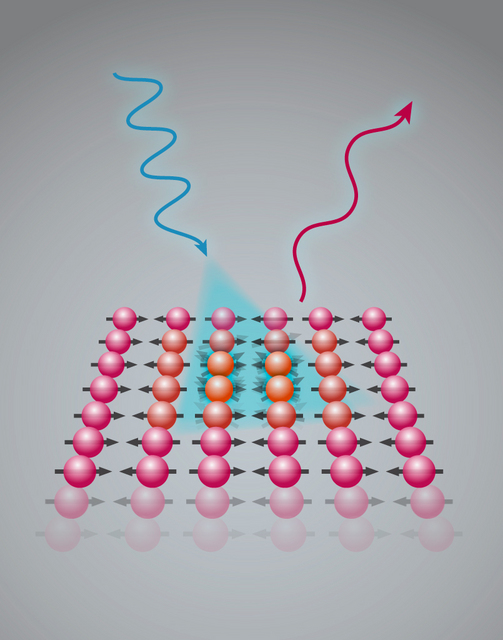
\includegraphics[scale=0.9]{IMG/copertina.jpg}
\end{center}

\newpage
\tableofcontents
\newpage

\section{Fisica della Materia e della Radiazione}
Si definisce \textbf{Materia Condensata} un insieme di particelle interagenti. In funzione del numero di particelle, è possibile avere strutture differenti:
\begin{itemize}
	\item Nanostrutture $[\text{nm}]$ = caratterizzate da poche particelle interangeti, sul centinaio $(<10^3)$. Ovviamente avendo pochi atomi si hanno sttrutture molto piccole;
	\item Mesostrutture $[\mu m]$ = caratterizate da un numero di particelle di $\sim  10^4$;
	\item Strutture macroscopiche $[mm]$ = sono caratterizzate da un $N_A$ di particelle interagenti.
\end{itemize}
Lo scopo del fisico è quello di costruire modelli fisici partendo dall'osservazione. L'osservazione di un determinato fenomeno induce una domanda alla quale si cerca di rispondere attraverso la costruzione di un modello fisico. Davanti a questa necessità nasce il grande dilemma: quando usare un modello classico? Quando uno quantistico? La risposta varia di caso in caso. La descrizione di una particella, intesa come pacchetto d'onda, può cambiare molto in funzione al contesto in cui è inserita infatti se si ha sovrapposizione saranno presenti effetti quantistici che non si possono trascurare (per esempio l'interazione di scambio).
\subsection{Motivazioni storiche rilevanti}
In questo caso è necessario introdurre il discorso sulla diffrazione, riprendendo alcuni sviluppi storici della fisica di inizio '900. De Broglie, nella sua tesi di dottorato, postula la duplice natura della materia (corpuscolare ed ondulatoria) associando quindi, ad un certo momento $p$ una lunghezza d'onda $\lambda$. La relazione che unisce le due grandezze è la nota \textit{equazione di De Broglie}
\newl{\boxed{\lambda_D=\frac{h}{p}=\frac{h}{mv}. }}
Unendo il tutto con il momento angolare quantizzato di Bohr si ottiene la tanto interessante, quanto oscura, formula
\newl{\boxed{L = pr = n\frac{h}{\lambda} r  = n\frac{h}{2\pi r}r = n\frac{h}{2\pi} = n\hbar}}
che nasconde un mondo del tutto inesplorato. In primis, si nota subito la mancata definizione del mezzo oscillante. De Broglie infatti lascia aperta la questione del mezzo che viene perturbato e esce un momento angolare in funzione di multipli interi di $\hbar$, come se le orbite di Bohr fossero occupate da un'onda di lunghezza d'onda di De Broglie. La prima tappa del percorso conoscitivo della materia passa atraverso la verifica dell'ipotesi delle onde di De Broglie. A tal proposito, gli esperimenti di diffrazione di elettroni sono i più gettonati. In modo opportuno si preparano fasci di elettroni che vengono fatti diffrangere su di un cristallo. Uno schermo fluorescente (o un qualsiasi tipo di detector) è posto ad una certa distanza dal cristallo e raccoglie l'immagine diffratta. 
\begin{figure}
	\centering
	\fbox{
		\begin{tikzpicture}[scale=1,auto=center]
			\draw [->] (0,4) -- (0,0) ;
			\node[] at (0,4.2)  {$Beam$};
			\node[] at (1,1.5) {$40eV$};
			\node[] at (2.2,2.5) {$54eV$};
			\node[] at (0.7,1) {$\varphi$};
			\draw [ultra thick] plot [smooth, tension=0.5] coordinates {(0,0) (0.7,0.1)  (1,0.3) (1.3, 0.9) (1.5,3.5) };
			\draw [ultra thick] plot [smooth, tension=0.5] coordinates {(2.2,1) (2.5,1.6) (2.55,1.78) (2.5,1.8) (2.4,1.8) (2.2,1.75) (1.6, 1.7) (1.7, 4)};
			\draw (1,0.15) -- (3,2.35);
			\draw[->] (0,0.9) arc (90:50:2);

		\end{tikzpicture}
	}
	\caption{Grafico dell'esperimento di Davisson-Germer. Viene plottata l'intensità degli elettroni scatterati contro l'angolo di scattering. Per $E=54eV$ si ha $\varphi=50^o$}
	\label{Davisson}
\end{figure}
Come si può notare in Fig.~\ref{Davisson}, per un'energia di $54eV$ si ha un picco di elettroni scatterati per $\phi=50^o$. Questo fenomeno lo si spiega solo pensando alla materia in modo ondulatorio, in quando, per la legge di Bragg, avrò scattering solo quando all'energia del fascio corrisponderà una lunghezza d'onda comparabile con quella del size del reticolo, che nel nostro caso è identificato dal passo del reticolo cristallino.
\subsection{Pacchetto d'onda}
Con la precedente premessa, il modo migliore per descrivere gli elettroni è attraverso  pacchetti d'onda non sovrapposti in cui $p\gg (\Delta p)$ e  $V/N \gg (\Delta r)^3$. In questo modo  è possibile usare un modello semi-classico rappresentato, come detto precedentemente, dalla lunghezza termica di De Broglie
\newl{\lambda_D=\frac{h}{p}=\frac{h}{\sqrt{2mE_C}} = \left(\frac{h^2}{3mK_BT}\right)^{\frac{1}{2}}}
con cui è possibile verificare che 
\newl{\frac{N}{V}\lambda_D^3 = \frac{N}{V}\left(\frac{h^2}{3mK_BT}\right)^{\frac{3}{2}}\ll 1.}
Si raggiunge la stessa conclusione partendo dal principio di indeterminazione di Heisenberg scritto nella ususale forma
\newl{\Delta r \cdot \Delta p \geq h.}
da cui è possibile ricavare
\newl{\frac{V}{N}p^3 \gg (\Delta r) \cdot (\Delta p) \geq h^3}
sapendo che $p=(3mK_BT)^{\frac{1}{2}}$ si ottiene nuovamente
\newl{\frac{N}{V}\left(\frac{h^2}{3mK_BT}\right)^{\frac{3}{2}}\ll 1.}
Un sistema può quindi essere modellizzato in modo classico per \textbf{densità} molto alte, \textbf{temperature} molto basse e \textbf{masse} molto piccole. Alcuni esempi sono dati da
\begin{itemize}
	\item Gas di idrogeno $[T\sim 0.26 K]$ sotto questa temperatura può essere modellizzato con le leggi classiche della cinetica dei gas;
	\item Elettroni di conduzione $[T \sim 1.8\cdot 10^5K]$ per modellizzare questo sistema è necessario usare modelli quantistici;
	\item Molti fotoni $(>10^3)$ si ha il campo elettromagnetico classico, quindi le equazioni di Maxwell;
	\item Pochi fotoni $(<10)$ si ha la QED (Quantum Elettro Dynamic).
\end{itemize}

\section{Richiamo sui solidi}
La materia che si presenta sotto il suo stato di \textit{solido} ha la caratteristica di essere completamente ordinata, gode di simmetria per alcuni angoli particolari e ci sono delle periodicità nella struttura. Sistemi solidi amorfi si conoscono per 0D (così detti \textit{quantum dot} ), 1D e 2D (così detti \textit{quantum well} come per esempio il grafene). Oltre ai sistemi amorfi ci sono i \textit{Quasi Cristalli}. Sono caratterizzati dall'avere simmetrie miste, per esempio parti con celle penatgonali miste a parte con simmetria sferica. Per osservare come la materia è aggregata, quali simmetrie sono presenti ed eventuali correlazioni le osservazioni che si possono fare riguardano le figure di diffrazione costruite facendo diffrangere radiazioni differenti. In funzione al passo del reticolo\footnote{E' vera questa cosa? C'è effettivamente una correlazione tra campione che voglio studiare e la relazione che scelgo per studiarlo? Credo proprio di sì.} si possono studiare diverse immagini di diffrazione costruite per esempio con raggi X($1 KeV \sim 10KeV$), con diffrazione di neutroni ($0,1 eV\sim 1 eV$) oppure strutture superficiali, diffrazione di elettroni ($100 eV$). A temperature prossime a quelle dell'ambiente ($T\sim 300K$) i neutroni hanno un loro momento magnetico. In questo modo, vedendo l'interazione tra i netroni e la mataria posso farmi un'idea sulle sue proprietà magnetiche. In conclusione, se devo studiare le proprietà magnetiche della materia uso neutroni a temperatura prossima a quella ambiente. 
\subsection{Reticolo di Bravais}
Un reticolo generico è possibile definirlo come 
\newl{\vet{R} = n_1 \vet{a} _2   + n_2 \vet{a} _2 + n_3 \vet{a} _3} 
in cui i vettori $\vet{a} _i$ non devono essere complanari. Il reticolo a nido d'ape, per esempio, non è un reticolo di Bravais perchè non è un gruppo puntuale.
bla bla bla (va aggiunta roba sui solidi)

\section{Teoria elementare della diffrazione}
Sia dato un certo sample da studiare come in Fig.~$\ref{Diff:1}$.
\begin{figure}
	\centering
	\label{Diff:1}
	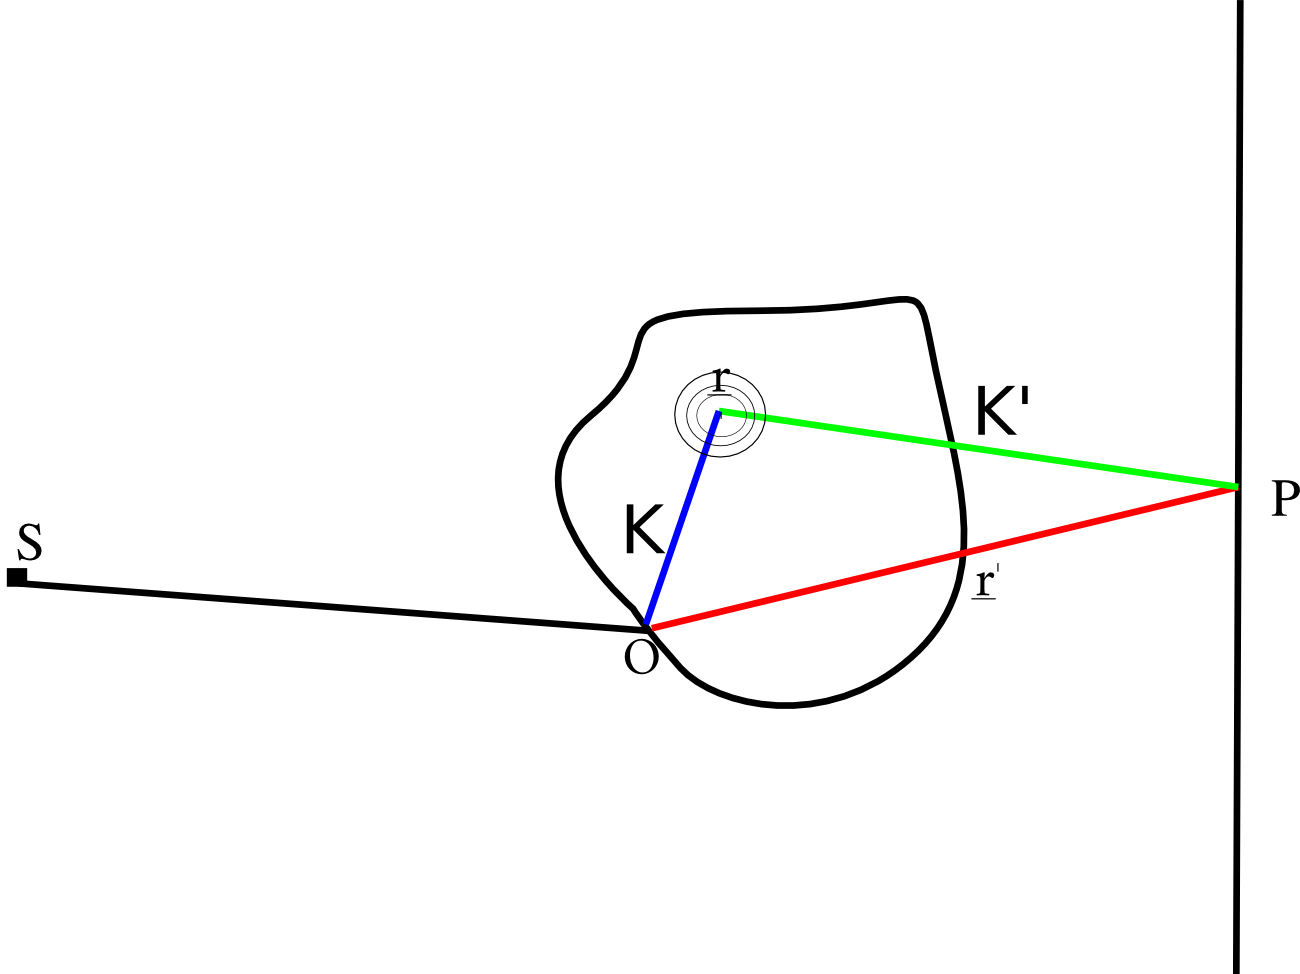
\includegraphics[width=120mm,angle=0,clip=]{IMG/Diff.png}
	\caption{Prova}
	\label{Diff:1}
\end{figure}
Consideriamo $S$ una sorgente puntiforme e continua, la radiazione colpisce l'oggetto nel punto $\xv{r} $. A sua volta diventa una sorgente di onde sferiche. Lo schermo si trova molto distante dall'oggetto colpito dalla radiazione, quindi $\abs{{\xv{r} }' }  \gg \abs{\xv{r} } $. La sorgente manda onde piane quindi
\newl{A(\xv{r} )=A_Se^{i[\xv{k} (\xv{r} + \xv{R} )-\omega t]}.}
Si considera solo lo scattering di una singola particella. L'onda interagisce con l'oggetto nel punto $\xv{r} $ generando onde sferiche che raggiungeranno lo schermo e verranno viste nel punto $P$. Le onde diffratte avranno come vettore d'onda $\xv{k} ' $. Quello che si vede nel punto $P$ sarà proporzionale a
\newl{A_P(\xv{r} )=\int d^3r A(\xv{r} )\rho(\xv{r} )\left(\frac{e^{i\xv{k} \cdot(\xv{r} '-\xv{r} )}}{|\xv{r} '-\xv{r} |}\right),}
dove $\rho(\xv{r} )$ è la densità elettronica nel punto di interazione. Sviluppando l'espressione del potenziale nel punto $P$ e raggruppando tutti i termini indipendenti da $\xv{r} $ ottengo
\newl{A_P(\xv{r} ) = \frac{A_Se^{i(\xv{k} \cdot \xv{R} + \xv{k} '\cdot \xv{r} ' -\omega t)}}{|\xv{r} '|} \int d^3r\rho(\xv{r} )e^{-i(\xv{k} '-\xv{k} )\cdot \xv{r} }.}
$A_P(\xv{r} ')$ è un integrale perchè va inteso come somma di tutte le onde piane generate dal punto $\xv{r} $ di interazione della radiazione incidente con l'oggetto. Quello che interessa è l'intensità delle spot sullo schermo, quindi si deve considerare il modulo quadro
\newl{I_P(\xv{r} )= \frac{|A_S|^2}{|\xv{r} |^2}\left|\int d^3r \rho(\xv{r} ) e^{-i \xv{q} \cdot \xv{r} } \right|}
dove $\boxed{\xv{q} = \Delta \xv{k} = \xv{k} ' - \xv{k} } $. Si può notare che $\int d^3r \rho(\xv{r} ) e^{-i \xv{q} \cdot \xv{r} }$ è la trasformata di fourire della $\rho(\xv{q} )$, quindi posso scrivere:
\newl{I_P(\xv{q}) = \frac{|A_S|^2}{|\xv{r} |^2}\left|\op{\rho} (\xv{q}) \right|}
Dato che l'obiettivo è quello di ricavare le distribuzioni elettroniche e dato che sullo schermo compare l'immagine della trasformata di fourier delle distribuzioni, a rigor di logica, antitrasformando si dorebbero ottenere le $\rho(\xv{r} )$. Questo non è possibile perchè l'evidenza sperimentale sullo schermo è data dal modulo quadro della trasfomata di Fourier, quindi mi manca il termine di fase per poter ricavare le distribuzioni nello spazio reale.

Per la trasformata di Fourier vale sempre che: $\Delta \xv{q} _x \cdot \Delta \xv{x} \sim \pi$ quindi si deve tenere in considerazione il fatto che per ottenere alte risoluzioni spaziali (quindi piccoli $\Delta \xv{x} $) mi servono grandi momenti $\xv{p} _x$.
\subsection{Reticolo Semplice}
\`E possibile applicare la teoria della diffrazione a modelli gradualmente sempre più complessi. Il primo modello che ci si presta ad affrontare è quello di un reticolo semplice. Il reticolo infatti è periodico con gli atomi vincolati nella loro posizione fissa. La distribuzione di carica elettronica è possibile quindi vederla espansa in serie di Fourier
\newl{\rho(\xv{r} )= \chi_V(\xv{r} ) \sum_{\xv{G} } \rho_{\xv{G} } e^{i\xv{G} \cdot \xv{r} }.}
Trasformo e ottengo 
\newl{\op{\rho} (\xv{q} )=\sum_{\xv{G} }\int_V \rho_{\xv{G} } e^{-i(\xv{G} - \xv{q} ) \cdot \xv{r} }.}
Possibili casi:
\begin{itemize}
	\item Se $\xv{G} \neq \xv{q} $: $\op{\rho} (\xv{q} ) =0$;
	\item Se $\xv{G} = \xv{q} $ : $\op{\rho} (\xv{q} ) = V\rho_{\xv{G} } \delta_{\xv{G} ,\xv{q} }$.
\end{itemize}
Quindi se $\xv{q}  = \xv{G} $ cioè $\xv{G} = \xv{\Delta k} = \xv{k'} - \xv{k} $ si hanno dei picchi, altrimenti il termine $\xv{G} - \xv{q} $ all'esponente dell'esponenziale complesso all'interno dell'integrale è molto grande. L'integrale di un esponenziale complesso, con argomento molto grande, ha media nulla quindi non sono visibili picchi. La regola:
\newl{\boxed{\xv{G} = \xv{\Delta k} = \xv{k'} - \xv{k} }} 
viene chiamata \textbf{\textit{condizione di Von Laue}}. 
\begin{figure}
	\centering
	\fbox{
		\begin{tikzpicture}[scale=1,auto=center]
			\node[fill=none] (n1) at (-0.25,0) {O};
			\node (n2) at (4.25,2) {$\xv{k'} $};
			\node (n3) at (4.25,-2) {$\xv{k} $};
			\node (n4) at (4.25,0) {$\xv{q} $};
			\foreach \from/\to in {n1/n2}
			\draw [->] (0,0) coordinate (a) -- (4,2) ;%node[draw=none,fill=none,font=\scriptsize,midway,below] {text below};
			\foreach \from/\to in {n1/n3}
			\draw [->] (0,0) -- (4,-2) coordinate (b)  ;%node[draw=none,fill=none,font=\scriptsize,midway,below] {text below};		
			\foreach \from/\to in {n3/n2}
			\draw [->] (4,-2) -- (4,2) coordinate (c) ;%node[draw=none,fill=none,font=\scriptsize,midway,below] {$\vet{q} $ };
			\draw [->] (0,0) -- (5,0);
			\draw (1,0) arc (0:30:1);
			\draw (1,0) arc (0:-30:1);
			\node[] at (15:1.25)  {$\theta_{1}$};
			\node[] at (-15:1.25) {$\theta_{2}$};
		\end{tikzpicture}
	}
	\caption{Scattering totalmente elastico.}
	\label{bragg}
\end{figure}
Dalla Fig.\ref{bragg} è possibile dedurre la legge di Bragg in quanto, anche in questo caso, lo scattering radiazione-materia è di tipo totalmente elastico. Scrivendo la condiozine di Von Laue ottengo che
\newl{\xv{G} = \xv{q} = \Delta\xv{k} \implicaa \abs{\xv{G} } = \abs{\Delta\xv{k} } }
considerando diffrazione per due piani paralleli:
\newl{\abs{G} = n\cdot \frac{2\pi}{d_{piani}}.}
Da Fig.\ref{bragg} si nota che a causa dello scattering completamente elastico si ha che $\theta_1 = \theta_2 = \theta$ quindi  $\abs{\xv{q} } = 2\abs{\xv{k} } \sin\theta$. Unendo le due precedenti riscritture del vettore $\xv{G} $ otteniamo la legge di Bragg
\newl{\boxed{\frac{4\pi\sin\theta}{\lambda} = n\frac{2\pi}{d_{piani}} \implicaa n\lambda = 2d\sin\theta . }}
Rimane ancora il fatto che se $\xv{q} =\xv{G} $ allora l'integrale ha dimensione di un $\rho_G \cdot V \delta_{{\vet q},{\vet G}} $ quindi l'intesità dell'immagine che vediamo sullo schermo risulta proporzionale a $I({\vet q}) \sim |\rho_G|^2 V^2 \delta_{{\vet q},{\vet G}}$. Non può essere proporzionale a $V^2$ è fisicamente impossibile in quanto la scrittura non torna dimensionalmente. La questione si risolve capendo che la funzione $\rho_G$ non è una funzione puntuale, ma ha una forma a spot di tipo campana gaussiana con piccole code. Effettuando l'integrale
\newl{\op{\rho} (\vet{q}) = \sum_G \int_V d^3r \rho_G e^{i(\vet{G}-\vet{q})\vet{r}}} 
è possibile arrivare ad un risultato che vede $I(\vet{q})\sim V$ che è fisicamente coerente.
\subsection{Un esempio più complesso: reticolo con base}
Un esempio più complesso può essere rappresentato dalla caratterizzazione dell'immagine di diffrazione da parte di un cristallo più complesso in cui abbiamo la sua rappresentazione tramite un reticolo e una base atomica. Il modo migliore per separare il problema è rappresentato in Fig.\ref{base:laue}.
\begin{figure}
	\centering
	\fbox{
		\begin{tikzpicture}[scale=1,auto=center]
			\draw [black] plot [smooth cycle] coordinates {(-1.5,-2.5) (-1,6) (5,6) (7,6) (7.5,4) (7,3) (6,-2)};
			\draw [->] (-1.5,-2.5) -- (0,0);
			\node (n1) at (-1,-1) {$\vet{R_n} $};
			\node (n2) at (0.25,0.45) {$\vet{r_\alpha} $};
			\draw [->] (0,0) -- (0.7,0.3);
			\draw (1,0.3) arc (0:360:0.3);
			\draw [->] (0.7,0.3) -- (0.7,0.6);
			\node (n3) at (0.9,0.65) {$\vet{r'} $};
			\draw [->] (-1.5,-2.5) -- (0.7,0.6);
			\node (n4) at (0,-1) {$\vet{r}$};


			\node[]  at (-1.7,-2.7) {O};
			\draw  (0,0) -- (4,0);
			\draw  (0,1) -- (4,1);	
			\draw  (0,2) -- (4,2);
			\draw  (0,3) -- (4,3);
			\draw  (0,4) -- (4,4);

			\draw  (0,0) -- (0,4);
			\draw  (1,0) -- (1,4);	
			\draw  (2,0) -- (2,4);
			\draw  (3,0) -- (3,4);
			\draw  (4,0) -- (4,4);

			\draw  (4,4) -- (6,5);
			\draw  (4,0) -- (6,1);
			\draw  (0,4) -- (2,5);

			\draw  (2,5) -- (6,5);
			\draw  (6,5) -- (6,1);

		\end{tikzpicture}
	}
	\caption{Sistema di riferimento di un cristallo complesso rappresentato da reticolo e base atomica.}
	\label{base:laue}
\end{figure}
Si prenda come origine un punto sul bordo dell'oggetto di forma generica. Il vettore $\vet{R}_n$ identifica la cella cristallina, il vettore $\vet{r}_\alpha$ identifica l'atomo $\alpha-esimo$ della base nella cella ed infine il vettore $\vet{r'}$ identifica la nuvola elettronica intorno all'$\alpha-esimo$ atomo. \`E  quindi possibile scrivere che
\newl{\boxed{\vet{r}=\vet{R}_n + \vet{r}_\alpha + \vet{r'}}.} Ovviamente $\vet{r}$ identifica un punto della nuvola elettronica dei vari $\alpha$ atomi che costituiscono la base della cella cristallina. Nell'integrale entra appunto solo il contributo delle nuvole elettroniche in quanto noi stiamo usando raggi $X$ che interagiscono con le nuvole elettroniche degli atomi. Calcoliamo in questo caso come è fatta l'immagine di diffrazione del cristallo passando sempre per la trasformata di Fourier della distribuzione di carica
\newl{\op{\rho} (\vet{q}) &=& \int_V d^3r\, \rho({\vet r})e^{-i{\vet q}\cdot {\vet r}} = \sum_{n_1,n_2,n_3}\sum_{\alpha} \int_Vd^3r'\,\rho_\alpha e^{-i{\vet q}\cdot({\vet R}_n + {\vet r}_\alpha + {\vet r'})}= \nonumber\\
			&=&\sum_{n1,n2,n3} e^{-i{\vet q}\cdot{\vet R}_n} \sum_\alpha e^{-i{\vet q}{\vet r}_\alpha} \int_{V_{cella}} d^3r'\,\rho_\alpha({\vet r}')e^{-i{\vet q}\cdot{\vet r'} }
}
in questo modo tutto si riduce all'integrale sul volume della $\rho(r')$ elettronica del singolo atomo. L'intensità è data sempre dal modulo quadro quindi è possibile scrivere
\newl{\boxed{I(\vet{q})=\overbrace{ \abs{\sum_{n1,n2,n3} e^{-i{\vet q}\cdot{\vet R}_n}} ^2 }^{\text{Fattore di Interferenza}} \overbrace{\abs{\sum_\alpha e^{-i{\vet q}{\vet r}_\alpha} \int_{V_{cella}} d^3r'\,\rho_\alpha({\vet r}')e^{-i{\vet q}\cdot{\vet r'} } } ^2 }^{\text{Fattore di Struttura}} }.}
Il Fattore di interferenza è diverso da zero solo per ${\vet q} = {\vet G}$ quindi, questa condizione, determina in che posizione avvengono i picchi. Il fattore di struttura, è quella parte che contribuisce all'allargamento del picco e rappresenta la trasformata di Fourier della densità elettronica dell'atomo $\alpha$ sulla cella. Questa parte è nota come \textit{Fattore di Forma Atomico}.
\begin{figure}
	\centering
	\fbox{
		\begin{tikzpicture}[scale=1,auto=center]
			\draw [->] (-1,0) -- (7,0);
			\draw [->] (0,-1) -- (0,7);
			\node (n1) at (7,-0.25) {${\vet q}$};
			\node (n2) at (-0.5,7) {$I({\vet q})$};
			\node (n3) at (1,-0.25) {${\vet G_1}$};
			\node (n4) at (2,-0.25) {${\vet G_2}$};
			\node (n5) at (3,-0.25) {${\vet G_3}$};
			\node (n6) at (4,-0.25) {${\vet G_4}$};
			\node (n7) at (5,-0.25) {${\vet G_5}$};
			\node (n8) at (6,-0.25) {${\vet G_6}$};

			\draw [red] plot [smooth, tension=0.2] coordinates {(0.5,0) (0.7,0.25) (1,4) (1.3,0.25) (1.5,0)};
			\draw [red] plot [smooth, tension=0.2] coordinates {(1.5,0) (1.7,0.25) (2,4) (2.3,0.25) (2.5,0)};
			\draw [red] plot [smooth, tension=0.2] coordinates {(2.5,0) (2.7,0.25) (3,4) (3.3,0.25) (3.5,0)};
			\draw [red] plot [smooth, tension=0.2] coordinates {(3.5,0) (3.7,0.25) (4,4) (4.3,0.25) (4.5,0)};
			\draw [red] plot [smooth, tension=0.2] coordinates {(4.5,0) (4.7,0.25) (5,4) (5.3,0.25) (5.5,0)};
			\draw [red] plot [smooth, tension=0.2] coordinates {(5.5,0) (5.7,0.25) (6,4) (6.3,0.25) (6.5,0)};

			\draw [green] plot [smooth, tension=1] coordinates {(-0.5,5) (3.5,5.7) (6.5,5)};

			\draw [green] plot [smooth, tension=0] coordinates {(4,7) (4.6,7)};
			\draw [red] plot [smooth, tension=0] coordinates {(4,6.5) (4.6,6.5)};

			\node[] at (6,7) {\fontsize{1mm}{1mm}\selectfont Fattore di Struttura};
			\node[] at (6,6.5){\fontsize{1mm}{1mm}\selectfont Fattore di Interferenza};
		\end{tikzpicture}
	}
	\caption{Fattore di Interferenza e Fattore di Struttura}
	\label{str:int}
\end{figure}
In Fig.\ref{str:int} sono rappresentati i contributi dei fattori di interferenza e struttura. Come è possibile osservare il fattore di interferenza è rappresentato da dei picchi situati in prossimità dei vettori $ {\vet G_n}$ e identificano le $N$ celle del reticolo cristallino.
\subsection{Un Liquido}
Supponiamo di indebolire il fatto che il reticolo sia cristallino. Supponiamo di avere a che fare con un oggetto che abbia le caratteristiche di un fluido. In questo caso fisso un ${\vet R} _n$ e sommo su tutti i vari ${\vet R} _m$. Devo quindi avere una funzione di correlazione spaziale che mi permetta di sapere in che posizione sono i vari ${\vet R} _m$ ripetto al mio punto fisso ${\vet R} _n$. Il fattore di interferenza diventa quindi 
\newl{T({\vet q}) &=& \abs{\sum_{n_1,n_2,n_3} e^{-i{\vet q} \cdot{\vet R}_n } }^2 = \sum_{{\vet R}_m = {\vet R}_n} e^{-i{\vet q}\cdot({\vet R}_n -{\vet R}_m)}+ \sum_{{\vet R} _n \neq {\vet R} _m } e^{-i{\vet q} \cdot({\vet R} _n- {\vet R} _m)} = \nonumber\\ &=& N + \sum_{{\vet R_n}} \left(\sum_{{\vet R} _n \neq {\vet R} _m}e^{-i{\vet q}(\vet{R} _n - {\vet R} _m)} \right) }
Estendo al continuo
\newl{T(\vet{q}) &=& N + N\int d^3r\, e^{-i{\vet q}\cdot(R_n-R_m)}P(R_n-R_m) = \nonumber\\
			       &=& N\left(1+\int d^3r\, e^{-i{\vet q}\cdot(R_n-R_m)}P(R_n-R_m)\right) 
}
Dove $P(R_n-R_m)$ è la funzione di correlazione spaziale che permette di studiare strutture non perfettamente regolari.


\section{Elettroni nel potenziale periodico}
Il problema agli autovalori che bisogna risolvere per trattare eletroni liberi in un potenziale periodico è il tipico
\newl{\left[-\frac{\hbar^2}{2m}\nabla^2 +U_e({\vet r})\right]\psi_n({\vet r}) = E_n \psi_n({\vet r}),}
dove si stanno facendo le seguenti approssimazioni:
\begin{itemize}
	\item Elettroni \textbf{indipendenti};
\end{itemize}
In questo modo la funzoine d'onda che descrive il problema è possibile fattorizzarla.
\begin{itemize}
	\item Il potenziale è periodico, quindi $U({\vet r}  + {\vet R} )  = U({\vet r}  )$
\end{itemize}
Il teorema di Bloch mi dice che per un potenziale periodico la funzoine d'onda è possibile fattorizzarla come una parte di onda piana e una parte periodica
\newl{\boxed{\psi_{n,\vet{k}}(\vet{r})=\overbrace{e^{i\vet{k}\cdot\vet{r}}}^{\text{Onda Piana}} \overbrace{u_{n,\vet{k}}(\vet{r}) }^{\text{Periodica}}}}
\subsection{Giustificazione fisica del teorema di Bloch}
La giustificazione del teorema di Bloch e quindi della forma delle funzioni d'onda dell'elettrone libero all'interno di un cristallo, trova la sua base sulle ipotesi fatte appunto sul reticolo del cristallo stesso. E' tutto periodico quindi mi aspetto che i moduli quadri della funzione d'onda siano periodici con passo quello del reticolo cristallino
\newl{\abs{\psi(r)} ^2 = \abs{\psi(r+R)} ^2,}
in questo modo, la funzione d'onda avrà una sua certa parte radiale con un certo coefficiente $C_{\vet k}$ per cui deve valere il fatto che $\abs{C_k} =1$. Un modo molto conveniente che ho di vedere questa cosa è quella di pensare appunto il coefficiente $C_{\vet k}$ dato da un'onda piana, infatti, cercando l'ugualianza tra le parti radiali di $\psi_k(r)$ r $\psi_k(r+R)$, notiamo che:
\newl{e^{ikr}\left[e^{-ikr} u_{n,k}(r)\right] = e^{ikr}e^{ikR} \left[ e^{-ikr}e^{-ikR}u_{n,k}(r+R)\right]}
da cui
\newl{\boxed{u_{n,k}(r) = u_{n,k}(r+R) }.}
In questo modo si vuole dare una giustificazione molto intuitiva del perchè le funzioni d'onda del teorema di Bloch sono funzioni d'onda sensate che seguono bene le condizioni di periodicità del nostro problema. Le soluzioni dell'hamiltoniana sono in funzione alle condizioni al bordo che scegliamo. In questo caso ha perfettamente senso scegliere delle condizioni al bordo periodiche. La restrizione sui valori di $\vet k$ sarà data da una serie di considerazioni. Partendo dalla periodicità $\psi(r) = \psi(r+L)$ sul reticolo, quindi se $a$ è un vettore del reticolo diretto si ha che $L = Na$. uguagliando le funzioni d'onda
\newl{e^{ikx} = e^{ik(x+L)} u_k(x+L)} 
ho come condizione
\newl{\boxed{kL = n 2\pi\implicaa k=\frac{2\pi}{L}n\,\,\, \text{ dove } \,\,\,n\in\Z }}
questa appena scritta è la famosa condizione periodica di \textit{\textbf{Born - Von Karman}}. Dal punto di vista dello spazio dei vettori $\vet k$ questo vuol dire che tutto quello che succede nello spazio può essere rimappato nell'intervallo di $k\in\left[-\frac{\pi}{a},\frac{\pi}{a}\right]$ che è appunto la prima zona di Brillouin. Nello spazio $k$ posso verificare facilmente che $k = k'-G$ dove $G$ è un vettore di base del reticolo reciproco
\newl{\psi_{k'}(x)e^{ik'x}u_{k'}(x) = e^{i(k+G)x}u_{k+G}(x)= e^{ikx}\overbrace{e^{iGx}u_{k+G}(x)}^{\text{Sono periodiche}}= e^{ikx}\op{u_k} (x).} 
In questo modo abbiamo confermato quanto detto prima. Ongi vettore $k'$ può essere rimappato all'interno della prima zona di Brillouin.
\subsection{Formazione delle bande}
Supponiamo di essere in condizione di potenziale debole a media nulla e che valgano le condizioni al bordo elencate precedentemente. Possiamo quindi trattare il problema agli autovalori come particella libera a cui viene successivamente inserito il contributo del potenziale debole in modo perturbativo. Il punto di partenza è banalmente la particella libera
\newl{\left(-\frac{\hbar^2}{2m}\nabla^2\right)  \psi_k(r) = E \psi_k(r).}
Con le condizioni al bordo periodiche, l'energia in funzione di $\vet k$ ha la tipica dipendenza quadratica
\newl{E=\frac{\hbar^2}{2m}k^2.}
\begin{figure}
	\centering
	\fbox{
		\begin{tikzpicture}[scale=1,auto=center]
			%\draw [help lines] (0,0) grid (2,2);
			\draw [->] (-5,0) -- (5,0);
			\draw [->] (0,-2) -- (0,5);
			\draw (-4,0.3*4^2) parabola bend (0,0) (4, 0.3*4^2);
			\draw (-2,0.3*4^2) parabola bend (2,0) (5, 0.3*3^2);
			\draw (-5,0.3*3^2) parabola bend (-2,0) (2, 0.3*4^2);
			
			\draw (0,0.3*4^2) parabola bend (4,0) (5, 0.3*1^2);
			\draw (-5,0.3*1^2) parabola bend (-4,0) (0, 0.3*4^2);
			\draw[domain=-1:1, ultra thick] plot (\x,{0.3*(\x)^2+1.2*\x+1.2});
			\draw[domain=-1:1, ultra thick]  plot (\x,{0.3*(-\x)^2+1.2*(-\x)+1.2} );
			\draw[domain=-1:0, ultra thick]  plot (\x,{0.3*(\x+2)^2+1.2*(\x+2)+1.2} );
			\draw[domain=0:1, ultra thick]  plot (\x,{0.3*((-\x)+2)^2+1.2*((-\x)+2)+1.2} );

			\draw[ultra thick] (-1,0.3) parabola bend (0,0) (1,0.3);
			\draw[ultra thick] parabola (-1,0.3) (1,9*0.3);	


			\node[fill,thick,circle, inner sep=0pt, minimum size=0.2cm] at (1,0.3)  {};
			\node[fill,thick,circle, inner sep=0pt, minimum size=0.2cm] at (1,9*0.3)  {};
			\node[fill,thick,circle, inner sep=0pt, minimum size=0.2cm] at (-1,0.3)  {};
			\node[fill,thick,circle, inner sep=0pt, minimum size=0.2cm] at (-1,9*0.3)  {};



			\node[] at (1.25,0.3)  {$1$};
			\node[] at (1.25,9*0.3)  {$2$};
			\node[] at (-1.25,0.3)  {$3$};
			\node[] at (-1.25,9*0.3)  {$4$};

			\node[fill,thick,circle, inner sep=0pt, minimum size=0.1cm] at (1,-0) {};
			\node[fill,thick,circle, inner sep=0pt, minimum size=0.1cm] at (-1,0)  {};
			\node[] at (1,-0.4) {$\frac{\pi}{a}$};
			\node[] at (-1.15,-0.4)  {$-\frac{\pi}{a}$};

			\draw[dashed] (-1,0) -- (-1,5);
			\draw[dashed] (1,0) -- (1,5);
		\end{tikzpicture}
	}
	\caption{Ritratto in fase dei momenti di particella libera}
	\label{Part:Lib}
\end{figure}
In Fig.\ref{Part:Lib}, è ben visibile che non vi è separazione tra le bande. \`E possibile passare in modo continuo da una banda all'altra nei punto in cui il vettore d'onda interseca la zona di Brillouin. in questo modo i punti $1,2,3,4$ hanno livelli quasi-degeneri, con energie di bande diverse che risultano molto vicine per lo stesso valore di $\vet k$. Si può passare ora a studiare il modo in cui il potenziale debole $U_e$ agisce sui livelli energetici. Il potenziale è riferito ad un reticolo diretto con una sua certa periodicità, è possibile rappresentarlo in serie di Fourier rispetto ai vettori $\vet q$ del reticolo reciproco 
\newl{U_e(x) = \sum_q U_q e^{i{\vet q}\cdot {\vet x}}\,\,\,\,\,\,\,\, \left(q=\frac{2\pi}{a}m\right).}
Adottando la convenzione di fissare la scala delle energie sul valor medio del potenziale allora si ottiene che $U_0=0$. Questo semplifica in modo essenziale gli sviluppi perturbativi. Riscrivendo l'equazione di Schroedinger con il contributo del potenziale
\newl{\left[-\frac{\hbar^2}{2m_e}\nabla^2+U_e(x)\right]\psi(x)=E\psi(x).}
A questo punto è necessario fare alcune considerazioni sulla funzione d'onda: essa può essere rappresentata sul sistema o.n.c delle onde piane, con opportuni coefficienti $C_k\in\C$
\newl{\psi(x)=\sum_kC_ke^{ikx}.}
Inserendo la funzione d'onda nell'equazione di Schroedinger appena scritta si ottiene il seguente problema agli autovalori
\newl{\sum_k\left[-\frac{\hbar^2}{2m_e}(-k^2)C_ke^{ikx}\right]+\sum_{q,k}U_qC_ke^{i(q+k)x}=E\sum_kC_ke^{ikx}}.
Moltiplicando per $e^{ik'x}$ ed integrando, si ottiene il seguente sistema per i coefficienti $C_k$
\newl{\left(\frac{\hbar^2}{2m_e}k^2 -E\right)C_k + \sum_q U_qC_{k-q} =0.}
Dall'ultima scrittura è possibile notare che il termine di potenziale è responsabile dell'accoppiamento tra i vari coefficienti $C_k$ infatti mette in realazione ogni coefficiente relativo ad un vettore $\vet k$ ad suo rispettivo nelle altre zone di Brillouin (che differenziano appunto di un vettore $\vet q$). Dato che può essere rimappato tutto nella prima zona di Brillouin, questo vuol dire che il termine di potenziale aggiunge accoppiamento tra i vari termini dello sviluppo. Tra i vari $\vet k$ vettori della prima zona di Brillouin si immagini di fissarne uno. In corrispondenza si avranno autofunzioni e autovalori indicizzati $\vet k$. Le funzioni d'onda dovranno essere la sovrapposizione di tutte le onde piane che distano di un vettore $\vet q'$ perchè come detto prima tutto viene rimappato nella prima zona
\newl{\psi_k(x)=\sum_{q'}C_{k-q'}e^{i(k-q')x}.}
Si noti che la somma è solo sui $\vet q'$ quindi è possibile riscrivere la funzione d'onda come
\newl{\psi(x)=e^{ikx}\sum_{q'}C_{k-q'}e^{-iq'x} = e^{ikx}u_k(x),}
questa forma è la stessa indicata per funzioni d'onda di elettrone libero in un potenziale cristallino dal teorema di Bloch. Questo fatto, con una certa forzatura, è possibile interpretarlo comeun'ulteriore prova a favore del teorema di Bloch. Prendendo la funzione d'onda appena scritta e usandola nell'equazione di Schroedinger si ottiene
\newl{\sum_{q'}\left[\frac{\hbar^2}{2m_e}(k-q')^2C_{k-q'}e^{i(k-q')x}\right]+\sum_{q',q"}U_{q"}C_{k-q'}e^{i(q"+k-q')x}=E_k\sum_kC_{k-q'}e^{i(k-q')x}}
Sfruttando nuovamente l'ortonormalità delle onde piane e integrando su $q"$ si ottiene, per ogni valore di $\vet k$, un sistema di equazioni accoppiate
\newl{\left[\frac{\hbar^2}{2m_e}(k-q)^2 -E_k\right]C_{k-q} +\sum_{q'}U_{q'-q}C_{k-q'}=0}
che una volta risolto fornisce i livelli energetici e i coefficienti dello sviluppo in serie della funzione d'onda. Ponendo $U_q=0$ si ritorna al caso precedente di particella libera
\newl{E_k,q = E(k-q)=\frac{\hbar^2}{2m_e}(k-q)^2}.
In questo caso $\vet q$ rappresenta il numero quantico che identifica la banda. Se ${\vet k} \sim {\vet q} /2$ si è in una condizione quasi degenere. Per valori di $\vet k$ lontani da questi punti le bande sono ben separate, il problema è solo in prossimità di questi punti. Per il calcolo della correzione dell'energia per mezzo di un potenziale debole è necessario considerare i due casi in modo separato e non si può effettuare una trattazione perturbativa standard. \`E possibile verificare che nel caso degenere per le due bande $q$ e $q'$ si ha 
\newl{\boxed{\Delta E=\abs{E(k-q)-E(k-q')}  \ll U .}}
Essendo la correzione dell'energia proporzionale a $U$  è quindi molto più significativa del caso non degenere in cui $\Delta E\gg U$ e la correzione di energia è proporzionale a $U^2$ quindi totalmente trascurabile. Ha quindi senso studiare solo la correzione dell'energia per il caso degenere poichè solo in questo caso si prevedono modifiche consistenti ai livelli energetici.
Per due bande degeneri generiche $\vet q_1$ e $\vet q_2$, tenendo conto solo dei termini dominanti si ottiene il seguente sistema algebrico
\newl{\left[E-E_{k,q_1}\right]C_{k-q_1} = U_{q_2-q_1}C_{k-q_1} \nonumber\\
	\left[E-E_{k,q_2}\right]C_{k-q_2} = U_{q_1-q_2}C_{k-q_2}
}
Soluzioni non nulle per i coefficienti dello sviluppo della funzione d'onda si hanno se si annulla il determinante della matrice
\[ \left| \begin{array}{cc}
E-E_{k,q_1} & -U_{q_2-q_1}  \\
-U_{q_1-q_2} & E-E_{k-q_2} \end{array} \right|.\]
Risolvendo per $E$ e osservando che $U_{q_1-q_2} = U^*_{q_2-q_1}$ (a causa del fatto che il potenziale è una funzione reale), si ottiene la correzione all'energia
\newl{\boxed{E(k)=\frac{E_{k,q_1}+E_{k,q_2}}{2}\pm \frac{1}{2}\sqrt{(E_{k,q_1}-E_{k,q_2})^2 + 4\abs{U_{q_1-q_2}} ^2 }   }.}
Questo indica che intorno a $(q_1+q_2)/2$ i livelli energetici di elettrone libero sono molto vicini e diventa molto singificativo il contributo del termine di potenziale. I livelli si \textit{respingono} dando vita ad un \textbf{gap di energia}, ovvero ad una zona di energie proibita. Possiamo notare che le correzioni all'energia diventano quindi sensibili quando $\abs{k-q_1} ^2 = \abs{k-q_2} ^2$ cioè quando siamo in una zona di quasi degenerazione. Posso ridefinire ${\vet k'} = \vet k - \vet q_1$ e $\vet q = \vet q_1 - \vet q_2$ in questo modo posso riscrivere la condizione di quasi degenerazione come
\newl{\abs{\vet k'} = \abs{{\vet k} - {\vet q}} }
cioè 
\newl{\boxed{\Delta{\vet k} = {\vet q}}}
che è la condizione di diffrazione di Von Laue. Quindi si spiega il motivo per il quale le bande si aprono in prossimità di quei punti, gli elettroni non possono stare in quelle posizioni e vengono diffratti.
\subsection{Soluzione elettrone libero in un potenziale periodico}
Nel paragrafo precedente sono stati elencati una serie di riusltati sulla formazione dei gap energetici in corrispondenza dei punti di quasi degenerazione. E' stato possibile verificare che la correzione all'energia è sensibile solo in questi punti. Lontano dai punti di quasi degenerazione la correzione all'energia diventa di ordine $O(N^2)$ quindi totalmente trascurabile. Per completare il concetto viene presentata, in modo più formale, la correzione agli autovalori per un elettrone libero in un potenziale periodico debole. Si consideri un potenziale realistico del tipo
\newl{V(x)=\sum_n v(x-na).
\label{PER:POT}}
La prima osservazione che è possibile fare è che il teorema di Bloch ci permette di separare, per ogni valore di $k$, il problema in due parti indipendenti. Si inizi col sostituire nell'equazione di Schrodinger la funzione d'onda di elettrone libero data dal teorema di Bloch
\newl{\left[-\frac{\hbar^2}{2m_e}\nabla^2 +V(x)\right]e^{ikx}u_k(x) = Ee^{ikx}u_k(x),}
in questo modo otteniamo un'equazione per la parte periodica
\newl{\left[\frac{\hbar^2}{2m_e}\left(k^2-2ik\frac{d}{dx}-\frac{d^2}{dx^2}\right)+V(x)-E\right]u_k(x)=0}
che in generale ha un'infinita di soluzioni ortogonali tra loro e sono del tipo
\newl{\int_{-L/2}^{+L/2}dx\,u^*_{k,n}(x)u_{k-m}(x) = \delta_{nm}N\int_{-a/2}^{+a/2}dx\,u^*_{k,n}(x)u_{k',m}(x).}
L'integrale è condotto su tutto il cristallo sfruttando la periodicità della funzione $u_k(x)$. L'integrale da $-L/2$ a $+L/2$ è stato quindi ricondotto alla sola cella unitaria.
Questo fatto è di interesse perchè mostra come è fatta la soluzione per quel tipo di problema e mette in luce che per valori di $k$ diversi, le soluzioni sono ortogonali tra loro. Riprendiamo gli stessi conti per una funzione d'onda di Bloch e sommiamo sempre su tutti i $k$ del reticolo
\newl{\int_{-L/2}^{+L/2} \psi^*_{k,n}(x)\psi_{k',n}(x)\,dx &=& \int_{-L/2}^{+L/2} e^{i(k'-k)x}u^*_{k,n}(x)u_{k',n}(x)\,dx \\
&=& \left(\sum_p e^{ip(k'-k)a}\right)\int_{-a/2}^{+a/2}e^{i(k'-k)x}u^*_{k,n}(x)u_{k',n}(x)\,dx ,	\nonumber}
i vettori p sono su tutto il reticolo e l'integrale è diverso da zero solo se $k$ e $k'$ coincidono, in questo modo si ha che
\newl{\sum_p e^{ip(k'-k)a} = N\delta_{k,k'}.}
In effetti non si può dire nulla sull'ortogonalità delle parti periodiche per diversi valori di $k$. L'unica cosa che si può dire è che per lo stesso valore di $k$, stati d'onda  di Bloch sono ortogonali.\footnote{Molto oscuro...}
\subsection{Metodo delle onde piane}
Il problema dell'elettrone libero in un potenziale periodico è possibile trattarlo in modo numerico. Dato il potenziale periodico, un approccio particolarmente efficace è quello di usare una base di onde piane, in particolar modo se il potenziale è periodico. \`E possibile definire a priori la forma di queste onde piane. Possiamo sfruttare la periodicità del reticolo e il teorema di Bloch che fissato un $k$, forniscono una forma particolare di base di onde piane
\newl{b_{n,k}(x)=\frac{1}{\sqrt{L}}e^{i(k+G_n)x}\,\,\,\, , \,\,\,\,\,\,\,G_n=\frac{2\pi}{a}n 
\label{BASE:BLOCH}}
la giusta base deve essere quindi del tipo $\exp(ikx)$ come stati di Bloch con vettori di Bloch $k$. Per un potenziale periodico come quello in formula \ref{PER:POT} abbiamo che la trasformata di Fourier è data da
\newl{\tilde{V}(G)=\frac{1}{L}\int_{-L/2}^{+L/2}V(x)e^{iGx}dx = \frac{1}{L}\left( \sum_p e^{ipGa} \right)\int_{-a/2}^{+a/2}v(x)e^{-iGx}dx }
e i vari componenti sono diversi da zero solo per un discreto insieme di vettori $G$, infatti il fattore $\sum_pe^{ipGa}$ è zero eccetto quando $Ga$ è un multiplo di $2\pi$, dove i $G_n$ sono quelli definiti in \ref{BASE:BLOCH}. In questo modo è possibile trovare
\newl{\tilde{V}(G)=\frac{1}{a}\int_{-a/2}^{+a/2} v(x) e^{-iG_nx}dx.}
L'integrale è calcolato per un singolo termine nel potenziale e in una singola cella unitaria. Al limite termodinamico, quindi per $N\to\infty$ questa cosa è ben definita.

\subsection{Legame Forte - Tight Binding}
Bho...

\subsection{Alcune considerazioni di carattere generale}
Risolvendo il problema degli elettroni liberi in potenziale periodico cristallino è stato possibile studiare il modo in cui si vengono a formare le bande di energia all'interno di un cristallo e e gli stati assunti dagli eletroni. In questo paragrafo si vuole mettere in risalto l'importanza di tutti i concetti precedentemente presentati e collegarli insieme per capire il modo in cui effettivamemente vengono usati in fisica. L'obiettivo principale è sempre quello di essere in grado, attraverso opportuni esperimenti, di determinare la struttura cristallina e le proprietà quantistiche del materiale in studio. Come visto precedentemente, il reticolo cristallino può essere ricostruito tramite diffrazione di Von Laue. Il teorema di Bloch, insieme alla soluzione del modello di elettrone libero in potenziale debole periodico, aggiunge l'informazione che i punti di diffrazione, trovati con la legge di Von Laue, sono punti di quasi-degenerazione per l'energia in cui l'elettrone potrebbe, in modo continuo, passare da una banda all'altra. Inserendo in modo perturbativo il contributo del potenziale è stato possibile vedere che si vengono a creare delle zone di energie non permesse. Quello che ci può dare un'idea concrete della forma della banda sono le superfici ad energia costante. Consideriamo quelle zone in cui il gradiente dell'energia è nullo e andaimo a studiarne la geometria
\newl{\nabla E(k) =0 \implicaa \frac{\hbar^2}{2m_e}\left(k^2-\left(\frac{q_1+q_2}{2}\right)^2\right)=0}
che è nulla in 
\newl{\boxed{k=\frac{q_1+q_2}{2}}.}
Questi valori di $k$ sono quelli che delimitano la Prima zona di Brillouin, quindi le superfici ad energia costante raggiungono la prima zona di brillouin con $\nabla E =0$ cioè sono normali alla superficie della zona.
\subsection{Proprietà vibrazionali dei solidi}
Nella sezione precedente ci si è concentrati sulla dinamica degli elettroni, visti come pacchetti d'onda che si muovono in un potenziale periodico. L'attenzione ora verrà spostata alle proprietà vibrazionali del reticolo. Il sistema cristallino viene sempre considerato con la solita approssimazione adiabatica. Elettroni e nuclei hanno scale di tempo di evoluzioni molto diverse quindi possiamo sempre separare lo studio delle due componenti, appunto moto degli elettroni e moto dei nuclei. L'Hamiltoniana del sistema da studiare è
\newl{-\frac{\hbar^2}{2}\left(\sum_i\frac{\nabla^2_{R_i}}{M_i}\right)\psi(R) + U_{\text{ad.}}(R) \psi(R) - E\psi(R) = 0.}
Dove con $i, j$ si identifica l'indice di particella, mentre con le lettere greche $\alpha, \beta$ si indentifica l'indice di direzione.
Supponiamo che $\vet R_0$ sia il punto di equilibrio di sistema, in questo caso posso sviluppare il potenziale adiabiatico in un intorno di $\vet R_0$ 
\newl{U_{\text{ad.}} =U_0 +  \sum_{i,\alpha,j,\beta} \left(\frac{\partial^2 U_{\text{ad.}}}{\partial u_{i,\alpha} \partial u_{j,\beta}}\right)_{R_0} u_{i,\alpha} u_{j,\beta} = U_0 + \Phi_{i,\alpha, j, \beta} u_{i,\alpha} u_{ j,\beta}  }
La $\vet \Phi$ è chiamata \textit{Matrice delle costanti di Forza} e rappresenta l'approssimazione parabolica del potenziale adiabatico lungo le varie direzioni, quindi le forze di richiamo, in approssimazione quadrata, lungo i vari assi. Per scrivere l'equazione del moto dei nuclei si passa dalla lagrangiana del sistema in cui i vari nuclei sono legati da una forza di richiamo, lungo le varie direzioni, indicata dalla matrice delle costanti di forza $\vet \Phi$. Se il numero di particelle è $N$ avrò $3N$ equazioni 
\newl{\mathcal{L}= \frac{1}{2}M_i(\dersf{u} _{i,\alpha})^2 - \frac{1}{2}  \Phi_{i,\alpha, j, \beta} u_{i,\alpha} u_{ j,\beta} }
per comodità di notazione sostituisco $q_{i,\alpha} = u_{i,\alpha}$ in questo modo posso scrivere le equazioni di Lagrange nella solita forma
\newl{\frac{d}{dt}\frac{\partial \mathcal{L}}{\partial \dersf{q} } - \frac{\partial \mathcal{L}}{\partial q}=0 }
derivando si ottengono le equazioni del moto
\newl{M_i \derrsf{u} _{i,\alpha}  + \Phi_{i,\alpha, j,\beta}u_{j,\beta} =0 .}
Nella prima parte, la ripetizione dell'indice $i$ nella matrice delle masse e nella parte di velocità non è da intendersi come somma covariante, in realtà $i$ è un indice libero che non si somma. Risolvo l'equazione differenziale nello spazio $\vet k$, passo quindi alla trasformata di Fourier 
\newl{k^2 {\vet M} u(k)  - {\vet \Phi} u(k) = 0.}
Definisco per semplicità $w = \sqrt{{\vet M}} u$, ottenendo
\newl{k^2 w - \left(\sqrt{{\vet M}}\right)^{-1} {\vet \Phi} \left(\sqrt{{\vet M}}\right) w =0 .}
La matrice ${\vet D} = \left(\sqrt{{\vet M}}\right)^{-1} {\vet \Phi} \left(\sqrt{{\vet M}}\right)$ è comunemente conosciuta col nome \textit{Matrice Dinamica}. Non è necessariamente diagonale quindi si trova un  operatore che sia in grado di diagonalizzarla. Si supponga che esista un operatore identificato dalla matrice $\vet S$ che goda delle seguenti proprietà
\newl{{\vet S}^\dagger {\vet S} = {\vet 1}, \text{e renda diagonale: }  {\vet S}^\dagger {\vet D} {\vet S} = 
	\left(\begin{array}{c c c}
		w_1^2&  &  \\
		 & \ddots &  \\
		 &  & w_N^2 \end{array}\right)
.}
Le coordinate degli autovettori di ${\vet D}$ sono
\newl{q={\vet S}^\dagger w \implicaa q = {\vet S}^\dagger {\vet M} ^{\frac{1}{2}} u \implicaa u = {\vet M}^{-\frac{1}{2}} {\vet S} q.}
Riscrivo la lagrangiana nella nuova base diagnonale
\newl{\mathcal{L} = \frac{1}{2} \dersf{w} ^\dagger \dersf{w} -\frac{1}{2} w^\dagger {\vet D} w = \frac{1}{2} \dersf{q} {\vet S^\dagger} {\vet S}\dersf{q} -\frac{1}{2} q {\vet S}^\dagger {\vet D}  {\vet S} q  ,}
essendo tutto diagonale posso scrivere la Lagrangiana in funzione di un singono indice
\newl{\sum_\gamma \mathcal{L}_\gamma = \frac{1}{2} \sum_\gamma \left[ \left(\dersf{q} _\gamma\right)^2 -k^2_\gamma q_\gamma\right].}
Effettuando il cambio di variabili $Q_\gamma = \sqrt{w_\gamma} q_\gamma$ ottengo
\newl{\mathcal{L} = \frac{1}{2}\sum_i \left[\frac{\dersf{Q} _i^2}{w_i}-w_iQ_i^2\right],}
che è praticamente la lagrangiana di un oscillatore armonico, infatti tramaite trasformata di Legendre arrivo quasi alla tipica Hamiltonina di un oscillatore armonico
\newl{H = \sum_i w_i \left(\frac{\op{P_i} ^2 + \op{Q_i} ^2}{2}\right)}
che, per come è stato impostato il problema,  è un risultato abbastanza aspettato. Usando gli operatori di salita e discesa\footnote{che sono definiti come: $\op{a} _i^\dagger =\frac{1}{\sqrt{2\hbar}} \left(\op{Q} _i - i\op{P} _i\right)$ e $\op{a} _i = \frac{1}{\sqrt{2\hbar}} \left(\op{Q} _i + i \op{P} _i\right)  $. }  arrivo esattamente all'Hamiltoniana di un oscillatore
\newl{H=\sum_i\hbar w_i \left(\op{a} _i^\dagger \op{a} _i +\frac{1}{2}\right).}
Quanto scritto vale per un sistema di $N$ atomi senza tener conto della periodicità del reticolo. Introducendo il fatto che il sistema è periodico con periodicità quella del reticolo, per la matrice delle costanti di forza vale la seguente scrittura
\newl{\phi_{i,n\alpha, j,n'\beta} = \phi_{i,(n'+n")\alpha, j,(n'+n")\beta} .}
Data la periodicità del sistema posso scrivere gli stati come stati di Bloch costituiti quindi da una parte periodica, con periodicità del reticolo, e da una parte di onda piana. Nello spazio di Fourier lo stato di block è
\newl{
	&&\tildato{W} _{i,n\alpha} = \sqrt{M_i} u_{i,n\alpha}\nonumber\\
	&&u_{i,n\alpha} = \frac{\tildato{W} _{i,n\alpha}}{\sqrt{M_i}} =  \frac{W_{i,n\alpha}}{\sqrt{M_i}} e^{ikR}
}
Sostituendo gli stati di Bloch nella Lagrangiana, tramite le equazioni di E-L arrivo ancora all'equazione del moto nello spazio $k$
\newl{
	&&k^2{\vet M} u -{\vet \Phi}u =0\nonumber\\
	&&k^2M_i\frac{W_{i,n\alpha}}{\sqrt{M_i}} e^{ikR_n} - \Phi_{i,n\alpha,j,n'\beta} \frac{W_{i,n\alpha}}{\sqrt{M_i}} e^{ikR_n}=0 
}
che usando la periodicità può essere riarrangiata in una forma più evidente
\newl{ \left(k^2W_{i,\alpha}({\vet k})  - \Phi_{i,\alpha,j,(n'-n)\beta} \frac{W_{j,(n'-n)\beta}({\vet k})}{\sqrt{M_j M_i}}\right) e^{ikR_n}=0  }
\subsection{Reticolo monodimensionale a due atomi}
Un esempio applicativo di quanto detto fin'ora è rappresentato dal reticolo monodimensionale con due specie atomiche.

\begin{center}
	\fbox{
		\begin{tikzpicture}[scale=1,auto=center]
			\draw (0,0) -- (1.75,0);
			\node[fill,thick,circle, inner sep=0pt, minimum size=0.2cm] at (0,0)  {};
			\node[draw, circle, inner sep=5pt, minimum size=0.1cm] at (2,0) {};
			\draw (2.25,0) -- (4,0);
			\node[fill,thick,circle, inner sep=0pt, minimum size=0.2cm] at (4,0)  {};
			\draw (4,0) -- (5.75,0);
			\node[draw, circle, inner sep=5pt, minimum size=0.1cm] at (6,0) {};
			\draw (6.25,0) -- (8,0);
			\node[fill,thick,circle, inner sep=0pt, minimum size=0.2cm] at (8,0)  {};


			\node[] at (2,0.45) {$2n-1$};
			\node[] at (4,0.45) {$2n$};
			\node[] at (6,0.45) {$2n+1$};
			\node[] at (4,-0.45) {$M_1$};
			\node[] at (6,-0.45) {$M_2$};

 			\draw (0,-0.3) -- (0,-0.6);
			\draw (2,-0.3) -- (2,-0.6);
			\draw[<->] (0,-0.45) -- (2,-0.45);
			\node[] at (1,-0.6) {$a$};


		\end{tikzpicture}
	}
\end{center}
I due atomi sono rappresentati dalle due diverse masse $M_1$ e $M_2$. La cella reticolare è di dimensione $2a$. Il fatto che siano presenti due tipi diversi di atomi questo permette di scrivere due equazioni del moto 
\newl{
	&&M_1 \frac{d^2u_{2n+1}}{dt^2} = -\alpha(2u_{2_n+1}-u_{2_n}-u_{2_n+2} )\\
	&&M_2 \frac{d^2u_{2n+2}}{dt^2} = -\alpha(2u_{2_n+2}-u_{2_n+1}-u_{2_n+3})
}
Dove $\alpha$ è la costante di accoppiamento interatomica, $n$ è un indice intero e scorre su tutti gli atomi di tipo $M_1$ quando è dispari e $M_2$ quando è pari. Le equazioni scritte sopra sono palesemente accoppiate. Abbiamo un totale di $2N$ equazioni differenziali accoppiate, da risolvere simultaneamente. Per risolvere questo tipo di equazioni si prende sempre in cosiderazione il sistema in studio e si formula un'Ansazt. Quella più attendibile è 
\newl{\left[\begin{array}{c}
		u_{2n+1} \\
		u_{2n}
\end{array}\right] = 
\left[\begin{array}{c}
	A_1e^{iqX_{2n+1}} \\
	A_2e^{iqX_{2n+2}}
\end{array}\right] e^{-i\omega t} .
}
In questo modo tutti gli atomi di massa $M_1$ hanno tutti ampiezza $A_1$ e lo stesso vale per gli atomi di massa $M_2$ che hanno ampiezza $A_2$. Sostituendo la soluzione del sistema di equazioni differenziali accoppiate scritto inizialmente, passando attraverso alcune drastiche semplificazioni si arriva alla semplice scrittura
\newl{\left(\begin{array}{cc}
		2\alpha - M_1\omega^2 & -2\alpha \cos(qa) \\
		-2\cos(qa) & 2\alpha -M_2\omega^2
	\end{array}\right) 
	\left(\begin{array}{c}
			A_1\\
			A_2
	\end{array}\right) = 0,
}
che è l'equivalente di due equazioni differenziali simulatanee nelle variabili $A_1$ e $A_2$. Le equazioni sono omogenee e hanno soluzione non banale solo se il determinante si annulla. La condizione diventa quindi
\newl{\text{det} \left|\begin{array}{cc}
	2\alpha - M_1\omega^2 & -2\alpha \cos(qa) \\
	-2\cos(qa) & 2\alpha -M_2\omega^2
	\end{array}\right| = 0.
}
A questa condizione corrisponde un'equazione nella variabile $\omega^2$ le cui soluzioni sono
\newl{\omega^2 =\alpha\left(\frac{1}{M_1} + \frac{1}{M_2}\right)\pm\alpha\sqrt{\left(\frac{1}{M_1} + \frac{1}{M_2} \right)^2 - \frac{4\sin^2(qa)}{M_1M_2}} .}
Come è possibile notare in Fig.~$\ref{PH:AC}$, in corrispondenza dei due diversi segni si distinguono due \textit{branches}, ottici e acustici.
\begin{figure}
	\centering
	\fbox{
		\begin{tikzpicture}[scale=1,auto=center]
			\draw[->] (0,0) -- (0,5);
			\draw[->] (-2.5,0) -- (2.5,0);
			\node[] at (0,5.3) {$\omega$};
			\node[] at (0,-0.25) {$0$};
			\node[] at (2,-0.25) {$\pi/2a$};
			\node[] at (-2,-0.25) {$-\pi/2a$};
			\draw[dashed] (2,0) -- (2,5);
			\draw[dashed] (-2,0) -- (-2,5);
			\draw[domain=-2:2] plot (\x,{3*sqrt((sin(\x*45))^2) });
			\draw[domain=-2:2] plot (\x,{3*sqrt((sin((\x+4.5)*20))^2)+1});
			
		\end{tikzpicture}
	}
	\caption{Fononi: bande acustiche e bande ottiche}
	\label{PH:AC}
\end{figure}
I rami acustici partono da $(0,0)$ e sono funzione crescente di $q$. Intorno a zero il comportamento è in prima approssimazione lineare, il che torna con le relazioni di dispersione lineare del suono nei mezzi, ben conosciuti in fisica calssica, la curva poi satura sui bordi della zona di Brillouin. Il ramo ottico invece, per $q=0$ vale 
\newl{\omega = \left[2\alpha\left(\frac{1}{M_1}+\frac{1}{M_2}\right)\right]^{1/2}} 
e descresce molto lentamente nell'avvicinarsi al bordo della zona di Brillouin. La frequenza di questo braccio non varia in modo apprezzabile lungo tutto il range di valori di $q$, infatti solitamente si considera costante. Il range di frequenze, tra la parte alta del ramo acustico e la parte bassa del ramo ottico, rappresenta una zona di frequenze non consentite. In questo range il cristallo non può trasmettere nessun tipo di onda. Il risultato che si ha è quello che ogni onda di frequenza proibita, che interagisce col cristallo, viene fortemente attenuata.

\section{Degenerazione degli stati}
Per studiare l'occupazione delle bande è necessario sapere quale distribuzione seguono gli elettroni nelle bande stesse. Il punto di partenza che consideriamo noto è la distribuzione di Fermi-Dirac:
\newl{n[E(k)]=\frac{1}{1+e^{\frac{1}{k_BT}(E(k)-\mu)}}}
dove $\mu$ indica il potenziale chimico da cui si deduce l'energia di Fermi come $\mu_{(T=0)}=\varepsilon_F$.
\begin{figure}
	\centering
	\fbox{
		\begin{tikzpicture}[scale=1,auto=center]
			%\draw [help lines] (0,0) grid (2,2);
			\draw [->] (-1,0) -- (5,0);
			\draw [->] (0,-1) -- (0,5);
			\node[] at (-0.7,4.5) {$n[E(k)]$};
			\node[] at (4.5,-0.25) {$E(k)$};
			\node[] at (-0.25,2.5) {$1$};
			\node[] at (2.5,-0.25) {$\mu_{(T=0)}$};
			\draw[] (-0.1,2.5) -- (0.1,2.5);
			\draw[] (0,2.5) -- (2.5,2.5);
			\draw[]	(2.5,2.5) -- (2.5,0);
			\node[] at (2.55,2.75) {$T=0$};
			\draw[blue,domain=0:5] plot (\x,{2.5/(1+ exp((\x-2.5)*2 )) });
			\draw[green,domain=0:5] plot (\x,{2.5/(1+ exp((\x-2.5)*3 )) });
			\node[] at (1,1.5) {$T\neq0$};
		\end{tikzpicture}
	}
	\caption{Distribuzione di Fermi in funzione di $E(k)$ e di $T$.}
	\label{Fermi}
\end{figure}
Come si può notare dalla Fig.\ref{Fermi} la distribuzione degli elettroni, in approssimazione di $T=0$ è una funzione gradino. Tutti i modelli che verranno studiati sono pensati a T=0. Se $f(E)$ è una funzione di distibuzione di una certa quantità, allora è necessario definire cosa si intende con quantità media di una grandezza fisica del sistema in esame. La definiamo come:
\newl{\langle A\rangle = \frac{1}{N}\sum_{stati}A(E)f(E) = \frac{1}{N}\int_0^{+\infty}dE\,g(E)A(E)f(E)}
dove con $g(E)$ si vuole indicare la \textit{degenerazione degli stati} cioè quanti stati sono presenti in un intervallo di energie $[E,E+dE]$. La funzione di degenerazione degli stati varia in funzione al problema. Per esempio per un elettrone libero di muoversi in un box cubico di lato $L$ (considerando $L\to\infty$ in questo modo tutte le somme sono integrali) con condizioni al contorno periodiche di Born-Von Karman, è possibile calcolare in modo esplicito la forma di g(E). Il punto di partenza è la funzione di partizione per un sistema di particelle. 
\newl{Z &=& \sum_{n_x,n_y,n_z} \exp\left[-\beta\frac{\hbar^2}{2m}\left(\frac{2\pi}{L}\right)^2(n_x^2+n_y^2+n_z^2)\right]=\int dn_x\, dn_y\,dn_z...=\\
&=&\int\,dEg(E)f(E) \nonumber}
E il punto è calcolare $g(E)$ che rappresenta il numero degli stati compresi tra $E$ e $E+dE$. Quindi posso definirla come
\newl{g(E)=\frac{dN}{dE}}
Il passaggio da somma ad integrale su tutti i possibili stati è possibile farlo grazie al fatto che $L\to\infty$.
E' stato fatto anche il seguente cambio di variabili passando dall'energia ai $k$ ed infine agli $n$
\newl{E=\frac{\hbar^2}{2m_e}k^2} 
dove i vari vettori $k_i$ vanno considerati con condizioni al bordo periodiche di Born-Von Karman, quindi 
\newl{k_i=\frac{2\pi}{L}n_i \implicaa \Delta n = \frac{L}{2\pi}\Delta k }.
Differenziando e sostituendo nella forma dell'energia per la particella libera ottengo che
\newl{dE = \frac{\hbar^2}{m}k\,dk.}
Ora calcolo l'integrale usando le coordinate sferiche
\newl{N= \int_{-\infty}^{+\infty} dn_x dn_y dn_z = \frac{L^3}{(2\pi)^2}4\pi\int_0^\infty dk\,k^2}
sostituisco con l'energia e ottengo
\newl{\frac{L^3}{(2\pi)^2}4\pi\int_0^\infty dk\,k^2 = \frac{L^3}{(2\pi)^2} \int_0^{\infty} dE\, \frac{m}{\hbar^2}\frac{\sqrt{2mE}}{\hbar} =\int dEg(E)}
quindi posso dire che
\newl{g(E)_{3D}=2_s\frac{V}{4\pi^2}\left(\frac{2m_e}{\hbar^2}\right)^{\frac{3}{2}}\sqrt{E}}
Siamo in approssimazione di $T=0$, quindi se vogliamo sapere il numero di elettroni con una certa energia $E$ l'integrale verrà taglaito all'energia di Fermi
\newl{N=\int_{-\infty}^{+\infty}dE\,g(E)_{3D}E = \int_0^{E_F} dE\,g(E)_{3D}E}
da qui ho la definizione dell'energia di fermi come:
\newl{E_F=\frac{\hbar^2}{2m}\left(3\pi^2\frac{N}{V}\right)^{\frac{3}{2}}}
\subsection{Degenerazione degli stati in una banda}
Nella sezione precedente è stato possibile calcolare la degenerazione degli stati per un modello di particella libera in uno spazio tridimensionale. Cerchiamo di estendere questo ragionamento applicandolo alle bande elettriniche dei solidi trovate in precedenza. Per estendere il concetto ad una banda elettronica partiamo nel definire la sommatoria su tutti gli stati come 
\newl{\sum_{n}\int_0^{+\infty}dEg_n(E)= 2\frac{V}{(2\pi)^3} \sum_n\int_{-\pi/a}^{+\pi/a} dk_x dk_y dk_z}
dove $n$ identifica il \textit{numero di banda}. L'obiettivo che quindi ci si pone è quello di trovare una formula generale per la $g_n(E)$ che indichi la degenerazione degli stati in funzione del numero di banda che compare come parametro, bisogna quindi avere una definizione di degenerazione degli stati per una banda. Per ottenerla si parte sempre dalla definizione generale precedente cioè, \text{numero di stati contenuti in un range di energie da $E$ a $E+\delta E$} con la particolarità di far rientrare in $E$ la struttura a bande. Consideriamo la Fig.~\ref{INTERVAL}
\begin{figure}
	\centering
		\begin{tikzpicture}[scale=3,auto=center]
			\draw [help lines] (0,0) grid (2,2);
			\draw (1,1) circle (0.2);
			\draw (1,1) circle (0.4);
			\draw[->, rotate around={315:(1,1)}](1,1.2) -- (1,1.4);
			\node[] at (1.3,1.1) {$\delta k$};

		\end{tikzpicture}
	\caption{Spazio $k$ con incremento di energia sufficientemente piccolo.}
	\label{INTERVAL}
\end{figure}
prendiamo nello spazio $k$ un'energia $E$ ed identifichiamo le sup. ad energia costante. Si identifichi un incremento $\delta k$ sufficientemente piccolo. A questo punto è possibile identificare la definizione di degenerazione degli stati di una banda, come nel caso 3D di particella libera, la definizione di $g_n(E)$ risulterà essere il numero di stati compresi nella corona circolare con estremi da $E_n$ a $E_n+(\hbar^2/m) k_n \delta k$. Definendo 
\newl{\chi_n(E)=1 \;\;\;\; \text{ se } E<E_n<E_n+dE \;\;\;\;\; \text{ else } \chi_n=0} 
è possibile scrivere la $g_n(E)$
\newl{g_n(E)dE=\frac{V}{(2\pi)^3}\int_{-\pi/a}^{+\pi/a} dk_x dk_y dk_z\chi_n = \frac{V}{(2\pi)^3}\int_{S_n(E)}dS\delta k}
dove $S_n(E)$ rappresenta la superficie della corona circolare. Sono superfici ad energia costante quindi
\newl{dE(k) = \abs{\nabla E_n(k)} \delta k}.
Inserendo tutto nella formula precedente si ottiene la scrittura della degenerazione degli stati nelle bande generalizzata al parametro di banda $n$
\newl{g_n(E)=\frac{V}{(2\pi)^3} \int_{S_n(E)}\frac{dS}{\abs{\nabla E(k)} } .}
\`E d'obbligo far notare che sulla superficie di Brillouin il gradiente dell'energia è nullo, annullando il denominatore dell'integranda. E' possibile comunque dimostrare che in 2D e in 3D l'integrale continua a convergere.
\subsection{Singolarità di Van Hove e regola d'oro di Fermi}
Riprendendo la forma delle degenerazione degli stati per una banda in un cristallo 
\newl{g_n(E) = \frac{V}{(2\pi)^3} \int_{S_n(E)}\frac{dS}{\abs{\nabla E(k)} } }
come da nota precedente è opportuno discutere il senso di questo integrale per zone vicine alle superficie della prima zona di Brillouin. Le superfici di energia costante intersecano in modo otogonale la superficie di Brillouin avendo, in quei punti, la condizione $\nabla E(k_{Brillouin}) =0$. I punti che soddisfano questa condizione sono chiamati punti di \textit{\textbf{singolarità di Van Hove.}} In questi punti il denominatore dell'integrale si annulla rendendo quindi obbligatoria una discussione della sua convergenza. Come è stato già detto precedentemente, si può dimostrare che in 2 e 3 dimensioni l'integrale continua a convergere. Direttamente collegato alla degenerazione degli stati è lo spettro di assorbimento otticodel cristallo. La probabilità di emissione è data dalla nota regola d'oro di Fermi
\newl{W_{if} = \frac{2\pi}{\hbar}\abs{\bra{i} H \ket{f} } ^2 \rho(\hbar\omega_{if} -\hbar\omega) }
dove con $i-f$ si intendono lo stato di inizio $(i)$ e lo stato di fine $(f)$ e con $W_{if}$ la probabilità di passare da uno all'altro. \`E presente anche una densità $\rho$ che idnetifica il numero di stati. Quindi la probabilità di fare emissione sarà in un qualche modo collegata alla densità di elettroni nella banda a quella determinata energia $\hbar\omega$. Se ne deduce che essendo le singolarità di Van Hove punti di divergenza dell'integrale, quindi punti in cui la funzione $g_n(E)$ è molto piccata, in quei punti è molto più favorita l'emissione di elettroni. Da notare come i punti di singolarità siano in prossimità dei punti di diffrazione idetificati nella teoria di Von Laue. L'elettrone arriva in quella zona di singolarità, particolarmente critico che ha una buona possibilità di essere emesso o difratto.

\begin{center}
\fbox{
\begin{tikzpicture}[scale=1,auto=center]
	\draw[->] (-1,0) -- (5,0);
	\draw[->] (0,-1) -- (0,5);
	\node[] at (5,-0.25) {$E$};
	\node[] at (-0.55,5) {$g_n(E)$};
	\draw (1,0) parabola bend (1,0) (3, 0.3*3^2);
	\draw (3, 0.3*3^2) parabola bend (3, 0.3*3^2) (4.5, 0);
	\node[fill,thick,circle, inner sep=0pt, minimum size=0.2cm] at (3,0.3*3^2)  {};
	\node[] at (3,0.3*3^2+0.25) {$\text{Singolarità di VH}$};
\end{tikzpicture}
}
\end{center}

\subsection{Esempi di elettrone vincolato}
Nella sezione precedente è stato possibile ricavare una forma generale per il calcolo della degenerazione delle bande. Di seguito si applicherà il concetto a diversi tipi di modelli quali \textit{quantum dot} e \textit{quantum well}.
\subsubsection{Quantum dot}
Il quntum dot, meglio conosciuto come atomo artificiale, è rappresentato da un sistema in cui gli elettroni sono vincolati in dimensioni molto piccole. La condizione di "zero dimensionalità" viene in un qualche modo suggerita dalla trasformata di Fourier e quindi dal principio di indeterminazione di Heisenberg. Se il lato del quantum dot, approssimato ad un cubettino molto piccolo, è $L$ questa sarà la nostra restrizione dimensionale $\Delta x$ a cui sarà associato un limite superiore di $\Delta p \sim \hbar/L$. Basandoci su questioni puramente morali possiamo scrivere il momento dell'elettrone come 
\newl{p\sim \frac{\hbar}{2L}}
considerando in questo modo anche la parte negativa di momento. L'energia dell'elettrone sarà quindi
\newl{E=\frac{p^2}{2m} = \frac{\hbar^2}{8mL^2}.}
Le dimensioni tipiche di un quantum dot sono nell'ordine di $L=10\text{nm}$. Usando $m_e$ risulta un'energia dell'elettrone di $E=0,1\text{eV}$. In realtà si utilizza la massa efficacie che fa risultare l'energia nell'ordine di $E\sim 10 \text{eV}$. Il problema si risolve sempre passando dal problema agli autovalori dell'equazione di Schroedinger risolta con condizioni al bordo di buca di potenziale. Già ora è possibile intuire che avendo delle condizione al bordo di tipo buca di potenziale lo spettro delle energie sarà molto diverso da quallo visto fino ad ora per elettrone libero con condizione al bordo periodiche di Born-Von Karman. Il fatto di avere delle condizioni di buca, potrebbe suggerire il fatto di avere un ground-state, che nei casi precedentemente visti non era presente. L'energia dell'ettone è possibile scriverla come
\newl{E_{n_x,n_y,n_z} = \frac{\hbar^2}{2m}(k_x^2+k_y^2+k_z^2)} 
dove i livelli sono discreti e separati da gap di energie nell'ordine dell'$eV$. C'è degenerazione, lo si nota anche semplicemente osservando che $E_{100} = E_{001}$. Quindi è necessario calcolare $g_{0D}(E)$. In questo caso è molto semplice, dato che le energie sono discrete sarà la somma dell'indice di degenerazione di ogni energia, che indichiamo con $g_j(E_j)$, per una delta di Dirac centrata sul valore dell'energia. Riassumendo il tutto
\newl{g_{0D}(E) = 2_s \sum_j g_j(E_j) \delta(E-E_j).}
\subsubsection{Filo quantico}
Il filo quantico è un altro modello utilizzato nella realtà per cui vale la pena valutare la degenerazione degli stati. \`E caratterizzato da $L_x \gg L_y,L_z$, quindi il problema si risolve  separandolo in due parti. Nella direzione $x$ l'elettrone è libero di muoversi, quindi in $x$ le condizioni al contorno, per il problema agli autovalori, saranno di tipo elettrone libero. Nelle direzione $y,z$ si ha invece confinamento, quindi le condizioni al contorno della funzione d'onda saranno diverse.
\begin{figure}
	\centering
	\fbox{
		\begin{tikzpicture}[scale=1,auto=center]
			\draw[->] (0,0.5) -- (0,2);
			\draw[->] (5,0) -- (6.5,0);
			\draw[->] (-0.35355,-0.35355) -- (-1.414,-1.414);
			\node[] at (-0.25,2) {$y$};
			\node[] at (6.5,-0.25) {$x$};
			\node[]	at (-1.214,-1.414)   {$z$};
			\draw[ultra thick] (-0.35355,-0.35355) -- (-0.35355,0.146466);
			\draw[ultra thick] (-0.35355,0.146466) -- (0,0.5);
			\draw[ultra thick] (0,0.5) -- (5,0.5);
			\draw[ultra thick] (-0.35355,-0.35355) -- (4.64645,-0.35355);
			\draw[ultra thick] (-0.35355,0.146466) -- (4.64645,0.146466);
			\draw[ultra thick] (4.64645,0.146466) -- (5,0.5);
			\draw[ultra thick] (4.64645,-0.35355) -- (4.64645,0.146466);
			\draw[ultra thick] (4.64645,-0.35355) -- (5,0);
			\draw[ultra thick] (5,0) -- (5,0.5);
		\end{tikzpicture}
	}
	\caption{Modello di filo quantico}
	\label{FILO:Q}
\end{figure}
Facendo riferimento alla Fig.~\ref{FILO:Q} possimao scrivere l'energia del sistema come
\newl{E = E_x + E_\perp = \frac{\hbar^2 k_x^2}{2m} + E(n_y, n_z).}
in $x$ ho la condizione di elettrone libero quindi le condizioni al contorno sono quelle di Born-Von Karman $k_x = n_x 2\pi/L_x$. Su $y$ e $z$ dato che ho confinamento le condizioni al contorno per la funzione d'onda rimarrano quelle di buca. Quindi il problema in questo modo si separa in due parti, su $y$ e $z$ la degenerazione degli stati rimande uguale al quantum dot
\newl{\boxed{g_{y,z}(E_\perp) = \sum_j g_j(E_j)\delta(E_\perp - E_j).}}
Sull'asse $x$ ho libertà quindi ottengo che
\newl{\sum_j \to  \frac{L_x}{2\pi} \int_{-\infty}^{+\infty} dk_x = \frac{L_x}{2\pi} \int_0^{+\infty} dk_x =\frac{L_x}{\pi}\int_0^{+\infty}dE\sqrt{\frac{m}{2E\hbar^2}}}
ottenendo quindi
\newl{g_x(E_x)=\frac{L_x}{\pi} \sqrt{\frac{m}{2\hbar^2}}\frac{1}{\sqrt{E}}.}
Unendo i risultati per ottenere una forma generale di densità degli stati si ottiene
\newl{g_{1D}(E)=\int_{0}^{+\infty}dE_x \int_{0}^{+\infty} dE_\perp g_x(E_x)g_{y,z}(E_\perp)\delta(E-E_x-E_\perp)}
Una cosa che non si capisce bene è la condizione per cui $\int dE_x \neq 0 \to E-E_\perp\geq0$. Con questa condizione definisco una funzione $\theta$ e posso elimanre l'integrale in $x$
\newl{g_{1D}(E)=\frac{L_x}{\pi}\sqrt{\frac{m}{2\hbar^2}} \sum_j g_j(E_j)\int_0^{+\infty} dE_\perp \frac{\delta(E_\perp-E_j)}{\sqrt{E-E_\perp}}\theta(E-E_\perp)} 
ma l'integrale è molto semplice e diventa quindi
\newl{g_{1D}(E)=2_s\frac{L_x}{\pi}\sqrt{\frac{m}{2\hbar^2}} \sum_j g_j(E_j)\frac{\theta(E_\perp-E_j)}{\sqrt{E-E_\perp}}.}
Lo stesso ragionamento lo si può estendere in modo molto semplice anche al caso di un sistema di "piano quantico". In questo caso il confinamento è solo su di un asse mentre sugli altri due ho la condizione di elettrone libero. La forma della degenerazione degli stati discende direttamente da quella del filo quantico
\newl{g_{2D}(E)=2_s\frac{L_xL_y}{2\pi}\frac{m}{\hbar^2}\sum_j\theta(E-E_j)}
\begin{figure}
	\centering
	\fbox{
		\begin{tikzpicture}[scale=1,auto=center]
			\draw[->] (0,-0.5) -- (0,5);
			\draw[->] (-0.5,0) -- (5,0);
			\node[] at (5.2,4.7) {$g_{3D}$};
			\node[] at (-0.6,5) {$g(E_k)$};
			\node[] at (5,-0.25) {$E_k$};
			%g_3D -> sqrt(E)
			\draw[blue,domain=0:5] plot (\x,{2*sqrt(\x)});
			%g_2D -> Cost.
			\draw[red] (0.2,0) -- (0.2,2*0.44721359549995793928);
			\draw[red] (0.2,2*0.44721359549995793928) -- (1,2*0.44721359549995793928);
			\draw[red] (1,2*0.44721359549995793928) --(1,2);
			\draw[red] (1,2) -- (3,2);
			\draw[red] (3,2) -- (3,2*1.732);
			\draw[red] (3,2*1.732) -- (5,2*1.732);
			%g_1D -> e^{1/2}
			\draw[green] (0,0) -- (0.5,0);
			\draw[green] (0.5,0) -- (0.5,5);
			\draw[green, domain=0.5:1.5] plot (\x,{7.071/sqrt(\x)-5}); 
			\draw[green] (1.5,{7.071/sqrt(1.5)-5}) -- (1.5,5);
			\node[] at (5,3.2) {$g_{2D}$};
			\node[] at (1.2,3) {$g_{1D}$};
			\foreach \p in {0,1,2,3,4} {
				\draw (\p,-0.1) -- (\p,0.1);
				\draw (-0.1,\p) -- (0.1,\p);
			}

		\end{tikzpicture}
	}
	\caption{Degenerazione degli stai per varie dimensioni. \`E ben visibile il comportamento della $g_{3D}\sim\sqrt{E}$ della $g_{2D}\sim\text{cost.}$ e della $g_{1D}\sim1/\sqrt{E}$. Per quando riguarda la $g_{0D}$ è banale perchè è costituita da una serie di delta centrate sulle energie degeneri.}
	\label{DEG:ST}
\end{figure}


\section{Dinamica degli elettroni in una banda}
Per descrivere la dinamica degli elettroni, in un certo tipo di potenziale, il primo passo è quello di identificare il modo migliore per descrivere l'elettrone stesso. In questo caso, l'approccio migliore è quello usuale, cioè la descrizione dell'elettrone tramite pacchetto d'onda sufficiente locacalizzato. Con sufficientemente localizzato si intende 
\newl{\psi_{\vet k}({\vet r},t) = \sum_{\vet k} f({\vet k})\exp\left[i\left({\vet k} \cdot {\vet r} - \frac{E({\vet r})}{\hbar}t\right)\right]}
in cui sia soddisfatta la condizione di minima incertezza
\newl{\boxed{\Delta {\vet r} \cdot \Delta {\vet k} \sim 1}.}
La lunghezza tipica su cui è scalato il problema, per quanto riguarda ${\vet k}$, è la dimensione della prima zona di Brillouin cioè $2\pi/a$. Avere un pacchetto d'onda ben definito nello spazio ${\vet k}$ vuol dire quindi avere un $\Delta {\vet k} \ll 2\pi/a$. Ovviamente, per continuare a valere la condizione di minima incertezza, se $\Delta k$ è molto piccolo, $\Delta x$ sarà molto grande, in questo caso sarà molto più grande di $\Delta x \gg a/2\pi$. Nel caso in studio è opportuno avere una buona definizione del pacchetto d'onda in $x$ (perchè?). Definiamo la \textit{velocità di gruppo} del pacchetto d'onda, che sarà data da
\newl{\boxed{\langle v \rangle = \frac{d\omega}{dk}=\frac{1}{\hbar}\frac{\partial E(k)}{\partial k}}}
Se abbiamo definito una velocità per il pacchetto d'onda allora possiamo dire che c'è una corrente che caratterizza il mezzo, la cui dentistà è
\newl{J=-e\int \frac{d^3k}{(2\pi)^3}2_s v(k)f(k)}
Se all'elettrone applico una forza, facendolo uscire dallo stato di equilibrio \`e possibile scrivere
\newl{dE = F dl = F \cdot v dt = F_\alpha v_\alpha dt }
La forza che agisce sul singolo elettrone sarà del tipo
\newl{F_\alpha = \hbar \frac{dK_\alpha}{dt}.}
In approssimazione semiclassica, l'equazione di newton per il singolo elettrone è possibile scriverla come
\newl{\frac{dv_\alpha}{dt} = \frac{1}{\hbar} \frac{\partial}{\partial t}\left(\frac{\partial E}{\partial k}\right) = \frac{1}{\hbar}\frac{\partial^2E}{\partial k_\alpha \partial k_\beta} \frac{\partial k_\beta}{dt}}
Osservando come è fatta la forma dell'equazione è possibile identificare le varie parti dell'equazione di newton e quindi definire una massa efficacie come 
\newl{\left(\frac{1}{m^*}\right)_{\alpha,\beta}=\frac{1}{\hbar}\frac{\partial^2 E}{\partial k_\alpha \partial k_\beta }}
che è strettamente in funzione alla forma della banda. La dinamica quindi è data dalla curvatura della banda. Se sono in una dimensione non ho problemi, se sono in più dimensioni \`e possibile avere masse efficaci diverse in funzione alla diversa curvatura della banda nelle varie direzioni. L'ordine di grandezza della massa efficace si aggira intorno a $0.01 m_e < m^* < 0.1 m_e$.
\subsection{Oscillazioni di Bloch}



Abbiamo visto che è possibile definire una velocità caratteristica del pacchetto d'onda all'interno del cristallo, associandola alla velocità di gruppo ${\vet v} = (1/\hbar) \partial_kE({\vet k})$. Se agisce una forza esterna sull'elettrone l'equazione del moto è possibile scriverla in forma semiclassica come
\newl{\boxed{a_\alpha =\left(\frac{d{\vet v}}{dt}\right)_\alpha = \left(\frac{1}{m^*}\right)_{\alpha,\beta}{\vet F} _\beta}}
spazio $k$ l'elettrone arriva a $\pi/a$ e riparte in modo periodico da $-\pi/a$. Quello che effettivamente succede è che nello spazio reale si ha un'inversione della velocità in prossimità dei punti di diffrazioni, quindi osservo delle oscillazioni, chiamate appunto oscillazioni di Bloch. Il profilo dell'energia e della velocità risulterà essere come in Fig~\ref{vel:en}.
\begin{figure}
	\centering
	\begin{subfigure}[b]{0.3\textwidth}
		\fbox{
		\begin{tikzpicture}[scale=1,auto=center]
			\draw[->] (-2,2.5) -- (2,2.5);
			\draw[->] (0,0) -- (0,5);
			\node[] at (2,2.25) {$k$};
			\node[] at (-0.5,5) {$E(k)$};
			\draw[dashed] (-1.8,0) -- (-1.8,5);
			\draw[dashed] (1.8,0) -- (1.8,5);
			\draw (-1.8,4.5) parabola bend (0,2.5) (1.8,4.5);
		\end{tikzpicture}
	}
		\caption{Grafico $E(k)$}
	\end{subfigure}
	\qquad\quad
	\begin{subfigure}[b]{0.3\textwidth}
		\fbox{
		\begin{tikzpicture}[scale=1,auto=center]
			\draw[->] (-2,2.5) -- (2,2.5);
			\draw[->] (0,0) -- (0,5);
			\node[] at (2,2.25) {$k$};
			\node[] at (-0.5,5) {$v(k)$};
			\draw[domain=-1.8:1.8] plot (\x,{2*sin(\x*180/1.8) + 2.5 });
			\draw[dashed] (-1.8,0) -- (-1.8,5);
			\draw[dashed] (1.8,0) -- (1.8,5);
		\end{tikzpicture}
	}
		\caption{Profilo della velocità}
	\end{subfigure}
	\caption{Velocità ed energia in funzione di  ${\vet k}$, $v_k = \hbar^{-1} \partial_k E$. Le linee tratteggiate indicano il confine della prima zona di Brillouin}
	\label{vel:en}
\end{figure}
Sperimentalmente la corrente di Bloch non si vede a causa delle impurità del cristallo. Se fosse visibile, la densità di corrente di Bloch avrebbe una forma tipica delle densità di corrente
\newl{{\vet J } = -e \int \frac{d^3k}{(2\pi)^3} 2_s {\vet v_k} f({\vet k}) \label{dens:corr}}
dove $f({\vet k})$ indica la densità di portatori di carica sulla banda. \`E abbastanza intuitivo capire che se $f({\vet k})=1$, cioè se la banda è piena, allora $\vet J = 0$ in quanto il profilo velle velocità sarebbe completo per ogni $\vet k$, integrando tutto nella prima zona di Brillouin, si integra $\vet{v_k}$ che è periodica dispari. Questo fa annullare l'integrale (\ref{dens:corr}). Se la banda è semipiena, ed è presente una certa forza esterna, allora in questo caso, per un cristallo perfetto, si ha ${\vet J} \neq 0$. La forza esterna è applicata inserendo il materiale in un campo elettrico, da questo fatto ecco giustificata la legge di Ohm
\newl{\boxed{{\vet J} = \sigma {\vet E}}}
Un ulteriore caso interessante è quello mostrato in Fig.~\ref{semip:cond} in cui si ha la banda di valenza quasi piena e la banda di conduzione con qualche elettrone.
\begin{figure}
	\centering
		\fbox{
		\begin{tikzpicture}[scale=1,auto=center]
			\draw[->] (-2,2.5) -- (2,2.5);
			\draw[->] (0,0) -- (0,5);
			\node[] at (2,2.25) {$k$};
			\node[] at (-0.5,5) {$E(k)$};
			\draw[dashed] (-1.8,0) -- (-1.8,5);
			\draw[dashed] (1.8,0) -- (1.8,5);
			\draw [black] plot [smooth,tension=0.4] coordinates {(-1.8,1.5) (-1.75,1.5) (-1.3,1.6) (0,2.5) (1.3,1.6) (1.75,1.5) (1.8,1.5)};

			\draw [black] plot [smooth,tension=0.4] coordinates {(-1.8,4) (-1.75,4) (-1.3,4.1) (0,3) (1.3,4.1) (1.75,4) (1.8,4)};

			\draw[->] (3,0) -- (3,5);
			\draw (3,1.2) -- (4,1.2);
			\draw (4,1.2) -- (4,2.5);
			\draw [black] plot [smooth,tension=1] coordinates {(4,2.5) (3.75,2.8) (3.15,3.25) (3,3.6)};	
			\draw[dashed] (0,3) -- (4.5,3);
			\draw[dashed] (-1.2,3.45) -- (4.5,3.45);
			\node[] at (3.5,0) {$f(E)$};
		\end{tikzpicture}
	}
	\caption{Esempio con banda di valenza pieno e banda di conduzione con pochi elettroni}
	\label{semip:cond}
\end{figure}


\begin{figure}
	\centering
		\fbox{
		\begin{tikzpicture}[scale=1,auto=center]
			\draw[->] (-2,2.5) -- (2,2.5);
			\draw[->] (0,0) -- (0,5);
			\node[] at (2,2.25) {$k$};
			\node[] at (-0.5,5) {$E(k)$};
			\draw[dashed] (-1.8,0) -- (-1.8,5);
			\draw[dashed] (1.8,0) -- (1.8,5);
			\draw [black] plot [smooth,tension=0.4] coordinates {(-1.8,1.5) (-1.75,1.5) (-1.3,1.6) (0,2.5) (1.3,1.6) (1.75,1.5) (1.8,1.5)};

			\draw [black] plot [smooth,tension=0.4] coordinates {(-1.8,4) (-1.75,4) (-1.3,4.1) (0,3) (1.3,4.1) (1.75,4) (1.8,4)};

			\draw[->] (3,0) -- (3,5);
			\draw (3,1.2) -- (4,1.2);
			\draw (4,1.2) -- (4,2.5);
			\draw [black] plot [smooth,tension=1] coordinates {(4,2.5) (3.75,2.8) (3.15,3.25) (3,3.6)};	
		\end{tikzpicture}
	}
	\caption{Esempio con banda di valenza pieno e banda di conduzione con pochi elettroni}
	\label{semip:cond}
\end{figure}

In questo caso la densità di corrente di Bloch è possibile scriverla come 
\newl{{\vet J} = 0 = -e \int\frac{d^3k}{(2\pi)^3} {\vet v} (k) f(k\pi) -e\int\frac{d^3k}{(2\pi)^3} {\vet v} (k) (1-f(k\pi) }
da cui si arriva all'ugualianza
\newl{e \int\frac{d^3k}{(2\pi)^3} {\vet v} (k) f(k\pi) = -e\int\frac{d^3k}{(2\pi)^3} {\vet v} (k) (1-f(k\pi) = {\vet J} _{semipiena} }
in cui la corrente nella banda semipiena è uguale alla corrente di buche cambiate di segno. La buca esiste solo nel materiale, non esiste come entit\`a a s\`e, quindi si definisce "quasiparticella". 
\subsection{Comportamenti oscillatori nei metalli}
La determinazione della superficie di Fermi cio\`e di quella superficie nello spazio $k$ delimitata dalle energie di occupazioni degli stati a bassa temperatura, \`e di particolare importanza nello studio della fisica dei metalli. La forma della superficie di fermi determina lo stato di equilibrio, le sue propriet\`a ottiche, i coefficienti di trasporto ed \`e il banco di prova per confrontare i calcoli teorici sulla struttura delle bande.
Circa le varie metodologie usate per indagare la forma della superficie di Fermi, quella che sfrutta \textit{l'effetto di De Haas - Van Alphen} \`e sicuramente quella pi\`u famosa e dal punto di vista fisico, strettamente collegata alle essenziali propriet\`a quantiche della materia condensata. L'effetto di De Haas - Van Alphen si pu\`o riassumere come \textbf{comportamento oscillatorio della magnetizzazione dei metalli (o semimetalli) come funzione di un campo magnetico applicato}.
L'effetto di De Haas - Van Alphen si presenza in quesi sistemi metallici molto puri, a temperatura molto bassa e tipicamente in presenza di campo magnetico molto forte, di alcuni Tesla. Le oscillazioni della magnetizzazione risultano da un fenomeno conosciuto come \textit{Quantizzazione di Landau} in cui gli elettroni in un metallo possono essere presenti solo solo su una serie di orbitali quantizzati in un campo magnetico. A causa del fatto che il numero di occupazione dei livelli di Landau cambia in funzione al campo magnetico applicato e quindi \`e possibile osservare oscillazioni nella manetizzazione ( o meglio, nella suscettivit\`a magnetica $\chi_M = \partial M / \partial H$ ) come previsto da Landau nel 1930. Queste oscillazioni sono esattamente periodiche con l'inverso del campo magnetico, come previsto da Onsager il quale ha permesso di collegare il periodo delle oscillazioni $\Delta(1/H)$ con l'area della sezione d'urto estremale della superficie di Fermi in un piano ortogonale alla direzione del campo applicato.

Gli esperimenti che indagano l'effetto di De Haas - Van Alphen, sono spesso caratterizzati da misure di voltaggio indotto in sensori arrotolati intorno al campione e a loro volta immersi in un grande solenoide che ne modula il campo magnetico interno. Il voltaggio nel singolo sensore \`e quindi proporzionale alla variazione di magnetizzazione nel tempo, quindi \`e anche un indice sulla suscettivit\`a magnetica. 
\subsection{Teoria semiclassica per elettroni di Bloch in campo magnetico uniforme}
Si consideri inizialmente una descrizione semiclassica della dinamica degli elettroni nelle bande energetiche. Gli elettroni sono rappresentati da pacchetti d'onda, come combinazione lineare di stati Bloch, piccati intorno ad un ben definito vettor d'onda $k$ e di una larghezza in modo tale che il pacchetto d'onda risulti distribuito su pi\`u celle del reticolo cristallino. La risposta all'applicazione di un campo elettrico o magnetico, che varia molto lentamente rispetto alla lunghezza del pacchetto d'onda da considerarlo constante in zone piccole del reticolo, \`e data da due equazioni della dinamica che collegano la velocit\`a dell'elettrone alla curvatura della banda energetica
\newl{\frac{\partial r}{\partial t} &=& v(k) = \frac{1}{\hbar} \frac{\partial E(k)}{\partial k}\\  
\hbar\frac{\partial k }{\partial t} &=& \frac{e}{c} v(k)\times H }
da cui segue immediatamente che l'energia $E(k)$ e la componente  del vettore d'onda $k$ parallelo alla direzione del campo magnetico, sono entrambe costanti del moto. Gli elettroni si muovono quindi lungo curve nello spazio $k$ (del reticolo reciproco) date dall'intersezione tra le superfici ad energia costante e i piani perpendicolari ad H. In particolare \`e possibile notare che si hanno orbite chiuse (non si \`e arrivati ancora al bordo della zona di Brillouin) e orbite aperte (\`e stata toccata la zona di Brillouin) in funzione alla geometria della superficie ad energia costante. In una teoria semiclassica la distribuzione delle orbite e dei livelli energetici \`e un quasi continuo e riflette la geometria delle superfici ad energia costante (questo non \`e totalmente vero in una teoria completamente quantistica).

Un importante risultato circa il moto di elettroni di Bloch in un campo magnetico che sar\`a molto utile \`e una \textit{relazione tra il periodo di un orbita chiusa e il cambiamento dell'area planare racchiusa dall'orbita, in fiunzione all'energia}. Partendo dall'equazione precedente scritta coi moduli
\newl{\abs{\frac{\partial k}{\partial t} } = \frac{|e|H}{\hbar^2c}\abs{\left(\frac{\partial E(k)}{\partial k}\right)_\perp }  }
dove $(\partial E(k)/ \partial k)_\perp$ \`e la componente del gradiente dell'energia perpendicolare al campo, in alre parole la sua proiezione sul piano dell'orbita. Il periodo di un orbita pu\`o essere determinato come 
\newl{T=\oint\,dt = \oint\frac{dk}{|\partial k / \partial t|} = \frac{\hbar^2c}{|e|H} \oint \frac{dk}{|(\partial E(k)/\partial k)_\perp|}}
dove  $dk$ rappresenta la quantit\`a di di una piccola orbita nello spazio $k$ e si sta integrando intorno ad un orbita chiusa. Se si vanno a considerare le orbite prime vicine, con differenza di energia $\Delta E = E_2-E_1$ piccola, La regione nel piano $k_x-k_y$ \`e una fascia di larghezza $\Delta(k)$, dove 
\newl{\Delta E = \abs{\left(\frac{\partial E(k)}{\partial k}\right)_\perp } \Delta(k)}
in cui il gradiente dell'energia \`e perpendicolare alla superficie ad energia costante e quindi, la sua proiezione \`e perpendicolare all'orbita. In questo modo il periodo pu\`o essere scritto come
\newl{T=\frac{\hbar^2 c}{\abs{e} H} \frac{1}{\Delta E} \oint\Delta (k) \,dk.}
L'integrale nell'ultima equazione rappresenta l'area tra le due orbite nello spazio $k$, definendo quest'area $\Delta A$, si arriva quindi alla fondamentale relazione
\newl{\boxed{T= \frac{\hbar^2 c}{\abs{e} H} \frac{\Delta A}{\Delta E}},}
in cui si mette in collegamento il periodo orbitale con la geometria della superficie ad energia costante nello spazio $k$. Nel limite della dinamica di elettroni liberi in banda, approssimazione valida per molti metalli, le superfici ad energia costante sono sfere e le orbite sono quindi circolari. Considerando l'energia dell'elettrone libero come $E(k) = \hbar^2 k^2 / 2 m $ l'area delle orbite nel pinao $k_x-k_y$ \`e $A=\pi k^2$, dato che in questo caso ha senso ricondursi al limite semiclassico, dal principio di corrispondenza di Bohr, deduco che
\newl{T=\frac{2\pi}{\omega_C}\,\,\,\,\,\,\,\,\,\,\,\,\,\,\,\, \omega_C = \frac{\abs{e} H}{mc}. \label{CICLOTR:OM}}
In questo modo \`e possibile mettere in relazione la variazione di area trasversale nello spazio $k$ tra orbite adiagenti (tubi di landau adiacenti) e il campo magnetico applicato
\newl{\boxed{\Delta A = \frac{2\pi \abs{e} H}{\hbar c} }.}
La $\omega_C$, definita in (\ref{CICLOTR:OM}), \`e la fondamentale \textbf{frequenza di ciclotrone}. Assomiglia molto alla $\omega$  classica per un elettrone in moto in campo magnetico, rappresentato, per\`o questa volta, nello spazio reale. 
Nella situazione in studio ora, l'energia ha una dipendenza quasi-parabolica dal vettore d'onda $k$, in questo modo le particelle cariche si comportano come particelle libere con frequenza
\newl{\boxed{\omega_C = \frac{\abs{e} H}{m^*c}},}
in cui $m^*$ rappresenta la \textbf{massa effettiva di ciclotrone}. La massa, quindi, pu\`o dipendere dalla direzione del campo magnetico applicato, che \`e collegato alla curvatura della superficie $E(k)$ e quindi in relazione con il tensore di massa efficace della banda.
Per campi magnetici nell'orgine di alcuni $KG$, la tipica frequenza di ciclotrone \`e nelle microonde. Per un campo magnetico di $1T$ e massa e carica dell'elettrone risulta $\omega_C=1.76\cdot10^{11} rad/s$ corrispondente alla lunghezz d'onda di $1.07cm$
\subsection{Livelli energetici di Landau}
Si vuole descrivere ora una trattazione quantistica dei livelli energetici di un sistema di elettroni liberi immersi in un campo magnetico costante. L'energia dei livelli di un sistema di particelle cariche immerse in un campo magnetico uniforme sono ovviamente diversi da quelli di particella libera. Si \`e particolarmente interssati all'energia dei livelli e alla loro distribuzione  nel sistema di elettroni in un metallo. Il primo approccio "geniale" \`e quello dei \textit{Livelli di Landau}.

L'Hamiltoniana del sistema \`e
\newl{\op{H} = \frac{1}{2m}\left(\op{p} -\frac{e}{c}A \right)^2 + e\phi - \mu\cdot H, }
dove $\op{p} $ \`e l'operatore momento dell'elettrone, $A=A(r)$ \`e il potenziale vettore del campo magnetico $H$. Siamo interessati ai livelli energetici di un gas di elettroni liberi in un campo \textbf{magnetostatico}, quindi $\phi=0$. Selezioniamo un campo magnetico diretto solo lungo l'asse $z$ quindi ${\vet H} =H\op{z} $ di modulo $H$. In generale l'operatore momento non commuta con il potenziale vettore infatti si ha che $[\op{p}, A] = -i\hbar\nabla\cdot A$, per\`o si pu\`o scegliere un potenziale vettore, costruito in modo tale che commuti con due componenti di $\op{p} $, che \`e $A = \left(A_x = -H\op{y}   ,A_y=0 ,A_z=0 \right)$, da cui si ottiene facilmente il campo magnetico desiderato (solo lungo l'asse $z$ con modulo $H$). In questo modo l'Hamiltoniana \`e possibile scriverla in modo decisamente pi\`u semplice
\newl{\op{H} = \frac{1}{2m} \left(\op{p} _x + \frac{eH}{c}\op{y} \right)^2 + \frac{\op{p} _y^2}{2m} + \frac{\op{p} _z^2 }{2m} -\mu_z H }
Dato che $[H,s_z]=0$ e dato che il problema \`e tutto concentrato sull'asse $z$ l'ultima parte dell'Hamiltoniana \`e possibile sostituirla direttamente son il suo relativo autovalore
\newl{E_{spin}= \pm \mu_B H = \pm \frac{1}{2} \hbar \omega_C}
cio\`e il contributo energetico di uno spin parallelo o antiparallelo al campo magnetico. Questo contributo energetico diventa rilevante solo se c'\`e un cambiamento nella distribuzione degli spin degli elettroni, come succede nel caso del paramegnetismo di Pauli, dove si hanno valori di suscettivit\`a magnetica piccoli e positivi. 

Escludendo quindi il contributo dello spin, l'equazione di Schroedinger per la funzione d'onda elettronica, nello spazio reale, \`e data da
\newl{\frac{1}{2m}\left[\left(\op{p} _x +\frac{eH}{c}\op{y} \right)^2 + \op{p} _y^2 + \op{p} _z ^2\right]\psi = E\psi. \label{SH:LAND}}
Le compomenti dell'operatore momento, $\op{p} _x$ e $\op{p} _y$ commutano con l'Hamiltoniana e quindi sono costanti del moto. I loro autovalori possono assumere \textit{a priori} valori da $-\infty$ a $+\infty$ senza limitazioni, come per esempio nel modello della particella libera, in cui la funzione d'onda \`e data da onde piane. In particolare, ricordando la relazione di come trasforma il momento in presenza di campi elettromagnetici $m{\vet v} = {\vet p} - (e/c){\vet A} $, si ha che $v_z = p_z/m$ e quindi risulta che la componente $z$ della velocit\`a risulta non quantizzata, mentre le altre componenti della velocit\`a possono essere determinate dagli autovalori dell'energia. Una soluzione per l'equazione (\ref{SH:LAND}) pu\`o essere la seguente ansatz
\newl{\psi(x,y,z) = \exp[i(xp_x+zp_z)/\hbar]\chi(y),}
dove $p_x$ e $p_y$ sono gli autovalori dell'operatore momento. Sostituendo tutto nell'Hamiltoniana, compresa la definizione dell'operatore $p_y=-i\hbar (\partial / \partial y)$, \`e quindi possibile scrivere
\newl{- \frac{\hbar^2}{2m} \frac{d^2\chi}{dy^2} + \left[ \frac{1}{2m}(p_x^2 + p_z^2) + yp_x \frac{eH}{mc} + y^2 \frac{e^2H^2}{2mc^2} \right]\chi = E \chi.  }
Introducendo la frequenza di ciclotrone ed introducendo il parametro $y_0 = -cp_x/(eH)$ si ottiene in conclusione il seguente problema agli autovalori
\newl{\left[ -\frac{\hbar^2}{2m} \frac{d^2}{dy^2} + \frac{m}{2}\omega_C^2(y-y_0)^2 \right]\chi(y) = \left(E-\frac{p_z^2}{2m}\right)\chi(y),}
che \`e praticamente l'equazione di Schroedinger per un oscillatore armonico monodimensionale, con $\omega = \omega_C$, centrato in $y_0$. La funzione d'onda e gli autovalori dell'energia, a questo punto, sono ben noti
\newl{E_n - \frac{p_z^2}{2m} = \hbar\omega_C\left(n+\frac{1}{2}\right)}
dove $n$ \`e intero e rappresenta il numero quantico riferito al corrispondente \textbf{Livello di Landau}, per un elettrone in moto in un campo magnetico uniforme. Riscrivendo meglio la relazione precedente
\newl\boxed{{E_{n_L}(p_z) = \hbar\omega_C\left( n_L + \frac{1}{2}  \right) + \frac{p_z^2}{2m}.}}






\section{Magnetismo nella Materia}
L'obiettivo del seguente capitolo è quello di introdurre una serie di proprietà di origine magnetica, quindi parleremo di \textit{Magnetismo nella materia}. A differenza degli aspetti macroscopici studiabili con i mezzi dell'elettrodinamica classica, ci si concentrerà sugli aspetti magnetici microscopici della materia e il loro collegamento col le variabili termodinamiche. Lo studio della materia sotto questo punto di vista ha permesso lo sviluppo di concetti quali: \textit{ordinamento spontaneo}, \textit{transione di fase} e \textit{approssimazione di campo medio}.
Partendo inizialmente dallo studio di paramagnetismo e diamagnetismo sarà possibile introdurre il concetto di \textit{approssimazione di particelle indipendneti} e successivamente passare allo studio delle \textit{correlazioni tra particelle in siti differenti} e quindi avere i mezzi di interpretazione del ferromagnetismo nella materia. Un possibile punto di partenza del discorso è sicuramente il teorema di Bohr - Van Leeuwen che afferma che la magnetizzazione nella materia ${\vet M}$ è sempre nulla. Nonostante questo sono evidenti i dipoli così come sono evidenti i fenomeni di ordinamento magnetico. Si inizi col definire la nomenclatura che verrà usata, per esempio tutto verrà scritto in unità c.g.s. In questo modo il campo di induzione magnetica è definito come
\newl{\boxed{{\vet B} = {\vet H} + 4\pi{\vet M}}}
dove con ${\vet M}$ si vuole identificare il vettore magnetizzazione che non è altro che il vettore di momento di dipolo di ogni singolo atomo, mediato sul volume, quindi una cosa del tipo
\newl{{\vet M} = \frac{{\vet \mu}}{V}.} 
Definisco la suscettività magnetica $\chi_M$ come 
\newl{\chi_M = \left(\frac{\partial M}{\partial H}\right)_{H=0}}
considerando in modo approssimato una relazione lineare tra $\vet M$ ed $\vet H$ e possibile scrivere che $M = \chi_M H$. \`E possibile riconoscere, in funzione al valore di $\chi$ diversi comportamenti della materia:
\begin{itemize}
	\item[1.] \textbf{Diamagnetismo}: caratterizzato da $\chi<0$, il sistema tende a "rifiutare" il campo applicato. Esempio: precessioni di Larmor;
	\item[2.] \textbf{Paramagnetismo}: caratterizzato da $\chi>0$, in questo caso se gli  atomi hanno un loro momento magnetico intrinseco, tendono ad allinearlo in direzione del campo;
	\item[3.] \textbf{Ferromagnetismo}: caratterizzato da fenomeni particolari quali \textit{magnetizzazione spontanea} e \textit{ordinamento}. I dipoli magnetici tendono ad orientarsi spontaneamente. In qeusto caso non vale più l'approssimazione lineare $M = \chi_M H$, in quanto il sistema sarà caratterizzato da transizioni di fase e in generale, da comportamenti abbastanza peculiari.
\end{itemize}
C'è un legame molto forte tra questi fenomeni e la temeperatura, quindi è opportuno fare una trattazione termidinamica. Si parte dall'enunciazione del primo principio:
\newl{dU = dQ - dW.}
Il lavoro per un genereico sistema immerso in un campo magnetico sarà dato, appunto, in parte da lavoro magnetico, una perte di lavoro meccanico e una parte di assorbimento dovuta all'eventuale scambio di particelle, indicando con $\zeta$ il potenziale chimico, 
\newl{dW = \mu\cdot dH + PdV - \zeta dN}
\begin{figure}
	\usetikzlibrary{arrows}
	\centering
	\fbox{
		\begin{tikzpicture}[scale=1,auto=center]
			\newcommand{\midarrow}{\tikz \draw[-triangle 90] (0,0) -- +(.1,0);}
			\draw[->] (0,-1) -- (0,5);
			\draw[->] (-1,0) -- (5,0);
			\node[] at (-0.2,-0.2) {$O$};
			\node[fill,thick,circle, inner sep=0pt, minimum size=0.2cm] at (3,3)  {};
			\draw (1,1) -- node {\midarrow} (2,1);
		\end{tikzpicture}
	}
	\caption{Forze in gioco}
	\label{Lorenz}
\end{figure}
Differenziando l'espressione dell'energia libera si ottiene che
\newl{dF = dU -d(TS) = -SdT -PdV +\zeta dN -\mu\cdot dH} 
e si ottengono tutte le relative grandezze in funzione di $F$ a $T$ $V$ ed $N$ fissati,
\newl{M = -\frac{1}{V}\left(\frac{\partial F}{\partial H}\right)_{T,V,N}\,\,\,\,\,,\,\,\,\,\,\chi = -\frac{1}{V}\left(\frac{\partial^2 F}{\partial H ^2}\right)_{T,V,N} .}
In meccanica statistica la funzione di partizione posso ottenerla anche dalla funzione di partizione canonica, che somma su tutti gli stati microscopici[\textbf{frase senza senso!!!}]
\newl{F = -k_BT\log Z \,\,\,\,,\,\,\,\, Z= \sum_{stati} e^{-H/k_BT}}
dove $k_B$ è la costante di Boltzmann e H è la classica Hamiltoniana di sistema. In alcuni casi è comodo scegliere il potenziale chimico come una rilevante variabile termodinamica, da cui si ottiene il potenziale \textbf{Gran Canonico}
\newl{\Omega = F -\zeta N = \Omega(T,V,\zeta,H)} 
a cui è associata una funzione di partizione gran canonica
\newl{Z_{\Omega}= \sum_{stati,particelle} e^{(\zeta N -H)/k_BT}}
dove la somma è appunto condotta su tutti gli stati e su tutte le particelle del sistema. Differenziando ottengo
\newl{d\Omega = dF -d(\zeta N) = -SdT -PdV -Nd\zeta - \mu\cdot dH}
da cui si derivano ancora le varibili osservabili del sistema
\newl{M = -\frac{1}{V}\left(\frac{\partial \Omega}{\partial H}\right)_{T,V,\zeta} \,\,\,,\,\,\, N =-\left(\frac{\partial \Omega}{\partial \mu}\right)_{T,V,H}}
Differenziando l'energia libera in funzione al gran potenziale canonico
\newl{\left(\frac{\partial F}{\partial H}\right)_N = \left(\frac{\partial(\Omega+\zeta N)}{\partial H}\right) = \left(\frac{\partial \Omega}{\partial H}\right)_\zeta + \frac{\partial \Omega}{\partial \zeta}\frac{\partial \zeta}{\partial H} + N \frac{\partial \mu}{\partial H}}
Come visto precedentemente la magnetizzazione è definita come una funzione di $\zeta$, quindi per ottenere la suscettività magnetica in funzione al numero di particelle si deve sempre partire dalla scrittura del gran potenziale canonico, rimaneggiarlo, ottenendo che
\newl{\chi = \left(\frac{\partial M(\zeta_{H,N}, H)}{\partial H}\right)_N = \frac{\partial M(\zeta,H)}{\partial H} + \frac{\partial M(\zeta,H)}{\partial \zeta}\frac{\partial \zeta}{\partial H}.}
Nella maggior parte dei casi, il potenziale chimico ha una dipendenza quadratica dal modulo del campo magnetico, quindi possiamo considerare $(\partial \zeta / \partial H) \sim 0$ e la suscettività data direttamente dalla formula
\newl{\chi = \left(\frac{\partial M}{\partial H}\right)_{H=0} = -\frac{1}{V} \left(\frac{\partial^2\Omega}{\partial H^2}\right)_\zeta.}
\subsection{Teorema di Bohr - Van Leeuwen}
Viene ripresa la tesi del teorema BVL e ampliata nei concetti. Come detto precedentemente, dal punto di vista della meccanica statistica classica, non sono ponderati i fenomeni magnetici nella materia, indipendenetemente da T e dall' {\vet H} applicato. Questo lo si può mostrare in modo semplice prendendo il valore medio di un'osservabile generica $F(r_i,p_i)$
\newl{\langle F \rangle = \frac{\int d^3r_i d^3p_i F(r_i,p_i) e^{-H(r_i,p_i)/k_BT}}{\left[\int d^3r_i d^3p_i e^{H(r_i,p_i)/k_BT}\right]} }
in presenza di campo magnetico, è risaputo che $p_i$  trasforma attraverso trasformazioni minimali $p_i \to p_i -(e/c)A(r_i) = p'_i$ mentre $r_i$ non cambia. Riscrivendo l'integrale di prima, la parte di potenziale vettore sparisce, perchè dipende solo dagli $r_i$ quindi ottengo che:
\newl{\langle F \rangle_{\text{senza A}}=\langle F \rangle_{\text{con A}}}
da cui si può dedurre che l'eventuale valore medio dell'osservabile $M$ con $H=0$, è uguale a quello per $H\neq0$ perchè il contributo del campo magnetico sparisce. Quindi ho che $\forall H$ 
la magnetizzazione di un sistema è sempre zero. Affermazione totalmente falsa, l'evidenza macroscopica del ferromagnetismo e delle transizioni di fase sono banali. Si conclude che un medello di meccanica statistica classica, non dice nulla riguardo i fenomeni magnetici. I fenomeni di ordinamento spontaneo sono fenomeni miscroscopici che vanno trattati in modo quantistico, infatti per prima cosa $\left[p,A\right]\neq 0$ ed in più va introdotto il concetto di dipolo magnetico intrinseco puramente quantistico, legato allo spin
\newl{\op{\mu_s} = g_s\frac{e}{2mc}\op{S} = -2\mu_B \op{S} \,\,\,,\,\,\,\op{S} _z=\pm\frac{\hbar}{2} }
\subsection{Hamiltoniana di Interazione Magnetica}
Come detto nel precedente paragrafo, il ferromagnetismo ed i fenomeni di ordinamento scpontaneo sono puramente quantistici, dunque il primo passo consiste nello scrivere l'Hamiltoniana del sistema in studio. Per un sistema di un elettrone immerso in un campo magnetico, si ha 
\newl{\op{H} = \frac{1}{2m}\left(\op{p} -\frac{e}{c}A(\op{r} )\right)^2.}
Per avere invarianza dei campi uso una gauge di Coulomb quindi con $\nabla\cdot{\vet A} =0$, che mi permette di scrivere il potenziale vettore e il campo come 
\newl{{\vet A} = \frac{1}{2} {\vet H} \times \vet{r}\,\,\, \implicaa\,\,\, {\vet H = \bf{\nabla} \times {\vet A} }}
in più, nella gauge di Coulomb ho che $\left[p,A\right]=0$. Riscrivendo l'Hamiltoniana di partenza diventa
\newl{\op{H} = \frac{\op{p} ^2}{2m} + \frac{e^2}{8mc^2}({\vet H} \times {\vet r})^2 - \frac{e}{2mc} \op{p} \cdot ({\vet H} \times {\vet r}) }
Supponendo che il campo magnetico sia diretto solo lungo l'asse $\op{z} $ e usando le seguenti relazioni vettoriali
\newl{
	({\vet H}\times {\vet r})^2 &=& H^2r^2 -({\vet H}\times {\vet r})^2 = H^2(x^2+y^2) \nonumber\\
	p\cdot({\vet H}\times {\vet r}) &=& {\vet H}\cdot {\vet r}\times {\vet p} = {\vet H}\cdot {\vet L} = H_z L_z
}
la parte cinetica dell'Hamiltoniana diventa 
\newl{H_c = \frac{p^2}{2m} + \frac{e^2}{8mc^2} H^2(x^2+y^2) -\frac{e}{2mc}L_zH}
il termine quadrato è dovuto al moto nel piano $x-y$, il termine lineare ha la forma di una energia di interazione tra il campo $\vet H $ e il momento di dipolo magnetico $\mu_l$ associato all'elettrone in orbita. In questo modo è ben distinguibile il comportamento paramagnetico, infatti considerando $l=L/\hbar$ ottengo
\newl{\mu_l = -\frac{\abs{e} \hbar }{2m}l = -\mu_B l}
che permette di scrivere l'Hamiltoniana di interazione 
\newl{H_{int} = -\mu_l H = +\mu_B l_z H = -\frac{e}{2mc}L_z H}
inserendo anche i contributi di interazione con campo elettrico, interazione del campo con lo spin e l'interazione spin-orbita ottengo l'Hamiltoniana totale di un sistema immerso in un campo elettromagnetico, definendo $\omega_c = (eH)/(mc)$ la omega di ciclotrone si ottiene
\newl{\op{H} = \frac{\op{p} ^2 }{2m}  + e\varphi(r)  + \frac{m}{8}\omega_c(x^2-y^2) + \mu_B l_z H + 2\mu_B S_z\cdot H +\xi(r) \op{L} \cdot \op{S}   }
le parti elettostatiche e di spin-orbita sono state aggiunte perchè l'elettrone è all'inteno di un atomo, quindi è soggetto anche a questo tipo di interazioni. \`E possibile ora discutere sui termini presente nell'Hamiltonianao. Il primo termine è quello cinetico, il secondo è quello di interazione con il potenziale elttrostatico, il terzo rappresenta lo sviluppo al prim'ordine dell'interazione col campo magnetico, il quarto rappresenta lo sviluppo al second'ordine sempre dell'interazione col campo magnetico, in quinto rappresenta l'interazione dello spin col campo magnetico ed infine si ha l'interazione spin-orbita. \`E possibile notare che \newl{\left[\frac{m}{8}\omega_c^2 (x^2-y^2) \right]  > 0}
quindi è un contributo repulsivo dimagnetico. Dal punto di vista delle grandezze fisiche, però ha un contributo di $\sim 10^{-10}eV$ che molto più piccolo del contributo dei termini quattro e cinque, che si aggirano sui $\sim 10^{-4}eV$ che rappresentano il contributo paramagnetico. Anche lo spin-orbita è di questo ordine di grandezza, $\sim 10^{-2}eV \to 10^{-4}eV$.
Poichè le energie dei livelli elettronici sono nell'ordine dell'$eV$ per eccitare un elettrone sarebbe necessario un campo magnetico gigantesco. In sostanza non è possibile eccitare gli elettroni tramite campi magnetici, quindi tutti gli effetti che sono legati all'interazione magnetica avvengono tutti nel ground state.
\subsection{Materiali Isolanti - Legge di Curie}
I materiali isolanti sono caratterizzati da atomi le cui bande sono piene. I numeri quantici utili per studiare questo tipo di sistemi sono $L,S,J$ totali, cioè $L=\sum_i l_i$ ecc... Dato lo stato $\psi_{r,s,j,j_z}$ il contributo paramagnetico è dato da
\newl{ \bra{J,J_z} L_z+2S_z \ket{J,J_z} = \mu_B Hg_LJ_z }
che è l'effetto Zeeman. Quindi per questi materiali la parte di Hamiltoniana di interazione sarà
\newl{\op{H} _{par} = \mu_B Hg_L\op{J} _z .}
Di notevole interesse è notare il fatto che l'intesità della correzione all'energia col contributo paramagnetico è nell'ordine di $10^4eV <k_BT$ ! Quindi sul sistema entrano in gioco anche le fluttuazioni dovute alla temperatura, che essendo dello stesso ordine di grandezza, non possono essere trascurate. \`E necessario quindi effettuare una trattazione del problema utilizzando i metodi della meccanica statistica. Come notato, si ha che $k_BT\sim10^{-2}eV \gg E_M$ quindi è necessaria una trattazione statistica. Il primo passo è quello del calcolo della funzione di partizione
\newl{Z=\sum_{stati}e^{-\frac{H}{k_BT}} = \sum_{-J}^{+J} e^{-\frac{\mu_B H g_L J_z}{k_BT}}}
ponendo $\gamma = (g_L \mu_B H) / (k_B T)$ e $J_z = n-J$ la funzione di partizione diventa
\newl{Z = e^{\gamma J} \sum_{n=0}^{2J}e^{-\gamma n} } 
che è molto facile sommare in quanto è una geometrica 
\newl{Z = e^{\gamma J} \frac{1-e^{-\gamma(2J+1)}}{1-e^{-\gamma}} = \frac{\sinh[\gamma(J+1/2)]}{\sinh(\gamma/2)}}
avendo a disposizione la funzione di partizione è possibile quindi passare alla determinazione di tutte le altre variabili termodinamiche del sistema. Di particolare interesse in questo capitolo è la determinazione della magnetizzazione
\newl{M = -\frac{N}{V}\frac{\partial}{\partial H}\left(-k_B T \ln Z\right) = \frac{Nk_BT}{V} \frac{1}{Z} \frac{\partial Z}{\partial \gamma} \frac{\partial \gamma}{\partial H}}
facendo i conti si arriva all'espressione della magnetizzazione in funzione alla funzione di Brillouin
\newl{M = \frac{N}{V}g_L \mu_B J \mathcal{B}_J\left(\frac{g_L\mu_BJH}{k_BT}\right)}
dove la funzione di Brillouin è una funzione adimensionale data da
\newl{\mathcal{B}_J = \frac{2J+1}{2J} \coth\left(x\frac{2J+1}{2J}\right)- \frac{1}{2J}\coth\left(\frac{x}{2J}\right)}
a temperatura ambiente l'energia magnetica è sempre più piccola dell'energia termica $(\mu_B H \ll k_BT \to x\ll 1)$ quindi è possibile espandere la $\coth(x)$ come  
\newl{\coth(x) = \frac{1}{x} + \frac{x}{3} + \cdots}
in questo modo si ottiene una espressione lineare per $M$
\newl{M = \frac{N}{V} \frac{g_L^2 \mu_B^2 J(J+1)}{3k_BT} H}
Infine si raggiunge l'espressione della suscettività paramagnetica di \textbf{Curie} in cui è visibile la dipendenza dall'inverso della temperatura
\newl{\chi_{para} = \frac{N}{V} \frac{(g_L \mu_B)^2 J(J+1)}{3k_B T}.}
Questo suggerisce che l'atomo può essere trattato come se avesse un suo proprio momento magnetico classico. La legge funziona molto bene per quegli ossidi che hanno la shell $f$ semipiena, mentre per le transizioni nei metalli funziona solo se sono verificate le condizioni $L=0$ e $J=S$. Per temperature molto basse e campi magnetici molto intensi il limite si inverte e si ha
\newl{x\to1 \,\,\,\, \coth(x)\to 1,}
e allo stesso modo si ha che la funzione di Brillouin tende ad $1$, $\mathcal{B}_J \sim 1$ e la magnetizzazione non dipende più da $H$ e si ottiene una magnetizzazione di saturazione
\newl{M=\frac{N}{V}g_L \mu_B J .}
Questa formula si interpreta facilmente dicendo che si raggiunge una situzione di saturazione, in cui tutti i momenti di dipolo di intensit\`a $g_L \mu_B J$ sono perfettamente allineati col campo $H$. Per alte temperature l'energia termica \`e molto pi\`u grande e i dipoli sono diretti equamente in tutte le possibili direzioni. Una stima numerica della magnetizzazione di saturazione, per una data densit\`a, che possiamo fissare a $N/V\sim 10^{22} atom/cm^{3}$, si aggira circa su $M\sim10^2 G = 10^{-2}T$. In pratica questo valore non viene mai raggiunto nei mezzi paramagnetici a temperatura ambiente, ma solo nei materiale ferromagnetici, infatti il paramagnetismo [\`e il piu grande effetto magnetico][ma che stai a d\`i?], ma la sua magnetizzazione e la sua suscettivit\`a magnetica hanno valori numerici molto piccoli, per esempio, per un campo di $H=1T$ si ottiene una $M\sim 1G$ e una $\chi \sim 10^{-4}$, giustificando l'assunsione che $B\sim H$.

Per quanto riguarda la scarsa valit\`a della legge di Curie per gli elementi di transizione della tavola periodica, in particolare gli atomi con una shell $d$ incompleta, questi atomi sono caratterizzare dall'avere orbitali molto estesi spazialmente anche oltre al raggio atomico. Questa particolarit\`a in una struttura cristallina potrebbe portare gli atomi ad interagire, via interazione Coulombiana con altri elettroni o ioni. Questa interazione potrebbe essere pi\`u intensa dell'interazione Spin-Orbita, in questo modo l'originale degenerazione sull'orbitale $d$ viene rotta.
Solitamente si considera una combinazione lineare di orbitali , corrispondenti gli stati nuovi con energie diverse (Crystal Field Splitting).In queste situazioni il momento angolare $L$ compie precessioni complicate all'interno del campo cristallino e la sua proiezione $L_z$ non \`e una costante del moto del sistema, quindi non \`e per nulla un buon numero quantico. Il valore di aspettazione delle proiezioni di $L$, tuttavia, sono $\langle L_x \rangle = \langle L_y \rangle = \langle L_z \rangle = 0$, risultato conosciuto come \textbf{Quenching del momento angolare orbitale}.
In pratica, per questo tipo di atomi in stato \textit{condensato} hanno $L=0$ e la legge di Curie \`e valida. Differente \`e il caso di per atomi in cui \`e presente la shell $f$ completa, ma gli stessi orbitali $f$ sono ben confinati spazialmente all'interno dell'atomo. I primi $4f$ orbitali iniziano ad essere riempiti dagli elettroni dopo il completamento dell'orbbitale $6s$ che \`e MOLTO ESTERNO. il Crystal field splitting \`e piccolo rispetto all'interazione all'accoppiamneto spin-orbita e le propriet\`a magnetiche dell'atomo sono molto simili a quelle di un sistema isolato. La legge di Curie rimane comunque valida in quanto il campo cristallino potrebbe originare piccole anisotropie magnetiche che conferiscono ai dipoli magnetici un orientamento preferenziale.
Casi speciali sono rappresentati dai cos\`i detti elementi di transizione. Possiamo identificare due diversi tipi:
\begin{itemize}
	\item Elementi con $J=0$ e $L = S \neq 0$;
	\item Elementi con $J = L = S = 0$.
\end{itemize}
\subsection{Elementi con $J=0$ e $L = S \neq 0$}
Questa situazione si verifica quando l'ultima shell ha un elettrone in meno per essere completata a met\`a. Un esempio diretto di questo fatto \`e lo ione di Europio $\text{Eu}^{3+}$ a bassa temperatura. Il contributo alla magnetizzazione al prim'ordine, usando l'Hamiltoniana effettiva \`e esattamente uguale a zero, quindi ci si appella al second'ordine perturbativo facendo diventare il contributo energetico
\newl{ \Delta E = - \sum_{n\neq0}\frac{ \left|  \bra{0} \mu_BH(L_z+2S_z) \ket{n} \right| ^2   }{E_n - E_0} }
dove $n$ rappresenta la collezione di numeri quantici particolarmente adatti dello stato eccitato del sistema. $\bra{0} $ rappresente il ground state e $\ket{n} $ rappresenta la funzione d'onda associata allo stato imperturbato di energia $E_n$. Da questa variazione di energia, proporzionale ad $H^2$ \`e possibile mettere in luce piccolissime suscettivit\`a paramagnetiche, praticamente indipendenti dalla temperatura. Questo fenomeno \`e conosciuto come \textbf{paramagnetismo di Van Vleck}. Queste oscillazioni sono molto difficili da osservare in quanto sono dello stesso ordine del contributo diamagnetico, che solitamente li maschera.
\subsection{Elementi con $J = L = S = 0$}
Sono tutti gli atomi con shell esterna completa. Questo \`e il caso in cui si studia il diamagnetismo. Il contributo magnetico all'energia \`e rappresentato solo dalla parte quadratica dell'Hamiltoniana effettiva. Il valore di aspettazione sul ground state \`e
\newl{\Delta E = \frac{m}{8} \omega^2_C  \bra{0} \sum_i(x_i^2 + y_i^2) \ket{0}    }
dove la somma \`e svolta su tutti gli $Z$ elettroni dell'atomo. Sfruttando la simmetria sferica del sistema, $x_i^2 = y_i^2 = z_i^2 = r_i^2 / 3$  \`e possibile riscrivere il contributo magnetico all'energia come 
\newl{\Delta E = \frac{e^2H^2}{12 m c^2} \bra{0} \sum_i r_i^2 \ket{0}  ,}
e la suscettivit\`a magnetica risulta
\newl{\chi_{dia} = -\frac{N}{V} \frac{e^2}{6mc^2} \bra{0} \sum_i r_i^2 \ket{0}  .}
Questo tipo di diamagnetismo \`e visibile nei gas nobili ed \`e l'esatto analogo classico del diamagnetismo di Larmor, dovuto al moto orbitale di particelle cariche. 
\subsection{Riassunto sugli elementi di transizione}
Riassumendo, se $J=0$,si ha che si annulla tutto, quindi devo passare al secondo ordine perturbativo attraverso la teoria di \textbf{Van Vleck}. Se $J=L=S=0$ allora tutti gli oggetti hanno suscettività diamagnetica. Sperimentalmente si osserva che per ioni con shell $f$ semipiena e $J\neq0$ l'accordo con la teoria è molto buono. Per gli elementi di transizione (shell $d$) la teoria non funziona per nulla. Per i casi in cui $J=0$ i il primo ordine perturbativo è nullo [\textbf{Non \`e vero !! Verificare....}]
\newl{\bra{\psi} \mu_BH(L_z+2S_z) \ket{\psi} = \mu_BHg_s J_z =0,}
devo usare il secondo ordine pertubativo rappresentato dalle oscillazioni di Van Vleck.


\subsection{Gas di Elettroni Liberi - Paramagnetismo di Pauli}
Nei metalli, i fenomeni di interazione con il campo elettromangetico sono dovuti per lo più dalla risposta degli elettroni liberi nelle bande di conduzione, al campo applicato. Gli effetti di magnetizzazione nei metalli sono caratterizzati da due coportamenti indipendenti:
\begin{itemize}
	\item Paramagnetismo di Pauli $\to$ dovuto all'allineamento dei dipoli magnetici col campo $\vet{H}$;
	\item Diamagnetismo di Landau $\to$ il secondo dovuto alla quantizzazione del moto degli elettroni immersi in un campo magnetico;
\end{itemize}
Gli elettroni nelle bande dei metalli hanno notevoli gradi di libertà quindi l'idea di trattare gli elettroni come un gas è ragionevole e d\`a risultati consistenti. Si calcolerà la suscettività paramegnetica di Pauli per un gas di elettroni. La derivazione può avvenire per vai statistica o per via variazionale, qui di seguito sarà argomentata la via statistica. Consideriamo l'ambientazione del problema in un sistema \textbf{gran canonico}. L'Hamiltioniana di riferimento \`e 
\newl{H=\frac{1}{2m^*} \left({\vet p} - \frac{e}{c}{\vet A} \right)^2 + 2\mu_BS_zH  }
con la parte cinetica data dall'interazione col campo magnetico e la seconda parte che rappresenta il termine paramegnetico di Pauli. La funzione di partizione, per particelle fermioniche, sarà quella gran canonica data da
\newl{Z_\Omega = \prod_{k_x,k_y,k_z,s_z} \left(1+e^{(\mu-E(k,s_z))/k_BT}\right). }
La produttoria è svolta su tutti i singoli stati degli elettroni con vettor d'onda 
$\vet{k} = \left(k_x,k_y,k_z\right)$ e spin $s_z$ aventi energia $E(\vet{k} ,s_z)$.
In assenza di campo magnetico, l'energia \`e quella di particella libera $E_0(k) = \hbar^2k^2/2m (k^2=k_x^2+k_y^2+k_z^2)$ per ogni proiezione dello spin lungo l'asse $z$. All'equilibrio termico met\`a degli spin saranno up e met\`a down. La funzione di partizione sar\`a $Z_0$, il potenziale gran canonico sar\`a $\Omega_0(\mu)$ dove $\mu$ rappresenta un adeguato potenziale chimico.
In presenza di campo magnetico $H$, l'energia si modificher\`a avendo in pi\`u il termine di interazione magnetica $-{\vet \mu_s} \cdot {\vet H} $, in particolare (all'equilibrio termico) gli elettroni con spin up, daranno un contributo all'energia pari $+\mu_BH$ mentre quelli con spin down $-\mu_BH$. L'energia degli stati sar\`a quindi 
\newl{E_{up/down} = E_0 \pm \mu_B H}
La funzione di partizione gran canonico ora dipender\`a dal campo magnetico. Pu\`o essere scritta separando le due famiglie di stati presenti
\newl{Z_{\Omega}(H) = \prod_{k_{up}} \left(1+e^{(\mu-\mu_BH-E_0(k))/k_BT} \right)\cdot \prod_{k_{down}} \left(1+e^{(\mu+\mu_BH-E_0(k))/k_BT} \right).}
Dalla differenza tra $Z_{\Omega} (H)$ e $Z_0$ la funzione di partizione gran canonica, alla fine, risulta dipendente solo dai due stati
\newl{\Omega(\mu,H) = \frac{1}{2}\Omega_0(\mu-\mu_BH) + \frac{1}{2}\Omega_0(\mu+\mu_BH).}
Il termine $\mu_BH \ll \mu$ (negli ordine di parecchi eV), quindi possiamo espandere la formula precedente in $\mu_BH$ ottenendo
\newl{\Omega(\mu,H) \sim \Omega_0(\mu) + \frac{1}{2}\mu^2_BH^2 \left.\frac{\partial^2\Omega}{\partial\mu^2}\right|_{H=0} }
dato che $N = - (\partial\Omega / \partial\mu)$ possiamo usarla nella formula della suscettivit\`a 
\newl{\chi_{pauli}= -\frac{1}{V} \frac{\partial^2\Omega}{\partial H^2} = \frac{1}{V} \mu_B^2 \left(\frac{\partial N}{\partial \mu}\right)_{T,V}  }
Per un sistema di fermioni posso facilmente calcolare $N$ come 
\newl{N = \int_0^{+\infty}dE\,g_{3D}(E)\left(1+e^{\frac{E-\mu}{k_BT}}\right)^{-1} = \int_0^{E_F}dE\,g_{3D}(E) = \frac{2}{3}\frac{V}{2\pi^2}\left(\frac{2m}{\hbar^2}\right)^{\frac{5}{2}}E_F^{\frac{3}{2}}}
in questo modo \`e possibile scrivere la sucettivit\`a di Pauli come
\newl{\chi_{pauli}=\frac{3}{2}\frac{N}{V}\frac{\mu_B^2}{E_F}  = \frac{3}{2}\frac{N}{V}\frac{\mu_B^2}{k_BT} .}
\textbf{N.B.} = $\chi_{pauli} \sim \chi_{para}/100$, questo \`e legato al principio di indeterminazione di Pauli. Considerando le sfere di fermi, solo gli elettroni vicini alle superfici possono riallineare lo spin, quelli interni non possono perch\'e gli stati con spin "dritto" sono gi\`a occupati. Solo una piccola parte di elettroni puo' cambiare segno. Al limite di $T \gg T_F$ si ritorna alla legge di Curie. [Capire bene perch\`e...]. 
\subsection{Gas di Elettroni Liberi - Diamagnetismo di Landau}
In questa sezione studieremo gli effetti che un campo mangetico ha sul moto libero degli elettroni nella banda di conduzione, indipendentemente dal loro spin. Fin'ora \`e stato visto che per il limite di temperatura molto bassa ($k_BT\ll\hbar\omega_C$) il tutto veniva spiegato con l'effetto di De Haas - Van Alphen. Ora verr\`a tolta questa condizione e si attaccher\`a il problema del magnetismo dell'orbitale elettronico per TUTTE le temperature, usando sempre i metodi della termodinamica e della meccanica statistica. I livelli energetici del sistema vengono dati dalla teoria di Landau, e sono quelli di un oscillatore armonico bidimensionale di frequenza angolare $\omega_C$ pi\`u un contributo di particella libera lungo l'asse $z$
\newl{E_n(k_z) = \frac{\hbar^2k_z^2}{2m} + \hbar\omega_C\left(n+\frac{1}{2}\right), }
mentre ogni levello ha una degenerazione data da 
\newl{N_d = \frac{|e|AH}{\pi\hbar c} = \frac{mA}{\pi \hbar^2}\cdot \hbar\omega_C}
dove $A$ rappresenza la superficie del campione [trasversale?? a cosa??]. La funzione di gran partizione diventa quindi
\newl{Z_\Omega = \prod_{k_x,k_y,k_z,s_z}\left[1+e^{\frac{\mu-E_n(k_z)}{k_BT}}\right].}
Per semplicit\`a introduciamo il parametro $\mu_z$ definito come 
\newl{\mu_z =  \mu - \frac{\hbar^2k_z^2}{2m}} 
e riscriviamo il gran potenziale come $\Omega = -k_BT\ln Z_\Omega = \sum_{k_z} \Omega'_z$ nella forma di una somma su di un due-dimensionale potenziale definito per un certo valore fisso di $k_z$ dove i vari $\Omega'_z$ sono definiti come 
\newl{\Omega'_z &=& -k_BT \sum_{k_x, k_y, s_z} \ln\left[1+e^{\frac{\mu_z-E_n}{k_BT}}\right] = \nonumber  \\
		&=& -N_dk_BT\sum_{n=0}^{+\infty} \ln\left[1+e^{\frac{\mu_z-E_n}{k_BT}}\right],}
dove $E_n=\hbar\omega_C(n+1/2)$ ed \`e stata introdotta la degenerazione degli stati perch\`e questo numero era stato esattamente calcolato come numero totale di stati elettronici permessi sulla superficie piana $A$ ad un fissato $n$. La dipendenza dal potenziale bidimensionale da $H$ \`e introdotta dalla frequenza di ciclotrone $\omega_C$ presente in $E_n$ e anche dal potenziale chimico, in cui, in realt\`a sarebbe un $\mu=\mu(H)$. Nella formula sopra la somma sulla tripla $\{k_x, k_y, s_z\}$ pu\`o essere pensata come somma su tutti i livelli energetici e su tutte le degenerazioni. Le degenerazioni le conosco dalla teoria di Landau. La somma scritta sopra si potr\`a notare che \`e possibile scriverla come integrali di termini oscillanti. Per ottenere dei risultati \`e necessario riscrivere la somma infinita come un integrale facile da calcolare. L'appossimazione che viene fatta \`e quella di ussare uno sviluppo in serie. La parte di particella libera non dipende dal campo H, la prima parte \`e la funzione di gran partizione per la particella libera in assenza di campo magnetico, solo la parte di oscillatore armonico conetiene una dipendenza da H quindi la parte di gran potenziale dovuta alla presenza di campo magnetico diventa
\newl{\Delta\Omega(H) = \sum_{k_z} \frac{mA\omega_C^2}{24\pi} \frac{1}{1+e^{\frac{-\mu_z}{k_BT}}}.}
In questo modo modo \`e possibile scrivere la funzione di partizione gran canonica e arrivare a calcolare la suscettivit\`a magnetica che risulta essere
\newl{\chi_L = -\frac{e^2}{12m\pi^2c^2}k_F = -\frac{1}{3}\frac{g_{3D}(E_F)}{V}\mu_B^2 = -\frac{1}{2} \frac{N}{V} \frac{\mu_B^2}{E_F}}
SI OSSERVI che la formula per la suscettivit\`a diamagnetica di Landau, ricorda molto quella paramagnetica di Pauli, in particolare il legame tra le due scritture \`e 
\newl{\boxed{\chi_L = -\frac{1}{3} \chi_P }}
dunque entrambi gli effetti concorrono con lo stesso ordine di grandezza alla risposta magnetica del gas di elettroni liberi che, in conclusione, \`e il modello pi\`u semplice per rappresentare la risposta magnetica dei metalli.

In questi sistemi il relativo peso del diamagnetismo contro il comportamento paramagnetico \`e fisso ad un $1/3$, ma esistono sistemi con un rapporto differente tra le due scuscettivit\`a. Si consideri un semiconduttore dopato (DS), in questo caso \`e presente un relativo minor numero di elettroni (o buche) nelle bande o vicini al comportamento di particella libera con massa effettiva $m^*$. La dipendenza della suscettivit\`a dalla massa segue dal fatto che nella $\chi_P$ \`e presente la densit\`a degli stati che $\partial N/\partial\mu=g_{3D}(E_F)\propto m$, in questo modo la suscettivit\`a paramegnetica scala come $\chi_P^{DS} = (m^*/m)\chi_P^{free}$.

Al contrario, nella $\chi_L$ la massa entra attraverso i livelli energetici di Landau che sono definiti da $E_n = \hbar\omega_C\left(n+\frac{1}{2}\right) \propto 1/m$, infatti il gran potenziale e $\chi_L$, sono inversamente proporzionali a $m$. Da queste osservazioni, nel caso di semiconduttori dopati, si ha che $\chi_L^{DS} = (m/m^*) \chi_L^{free}$.

In conclusione, per semiconduttori dopati, il rapporto tra le due suscettivit\`a risulta essere
\newl{\boxed{\frac{|\chi_L^{DS}|}{\chi_P^{DS}} = \frac{1}{3}\left(\frac{m}{m^*}\right)^2 ,}}
dato che tipicamente $m^* \sim 0.1m$ si ha che il comportamento diamagnetico diventa dominante rispetto a quello paramagnetico, e pu\`o essere direttamente misurato comparando il campione dopato con una non dopato.
\subsection{Fenomeni di Ordinamento Magnetico - Ferromagnetico}
Dal punto di vista sperimentale, sono evidenti in natura fenomeni di magnetizzazione spontanea in alcuni materiali di tranzione quali Fe, Co e Ni. I fenomeni di magnetizzazione persistono per temperature inferiori ad una certa temperatura critica (che pu\`o essere nell'ordine anche dei $10^3K$), oltre alla quale i materiali perdono totalmente le loro propriet\`a magnetiche. Allo stesso modo, la suscettivit\`a magnetica, mostra anche lei un comportamento divergente nei pressi della temperatura critica ($T_C$). Materiali che presentano questo tipo di comportamento si dice che presentano una \textit{transizione di fase del second'ordine}. L'evidenza di comportamenti magnetici da parte di alcuni materiali, in totale assenza di campo magnetico esterno, suggerisce che i dipoli magnetici atomici hanno un certo grado di allineamento ordinato in una certa collettivit\`a, meglio noto come \textit{ordinamento spontaneo}. Il Ferromagnetismo \`e il fenomeno  pi\`u diffuso di ordinamento magnetico, con rottura spontanea della simmetria spaziale del sistema in cui il parametro d'ordine \`e rappresentato dalla magnetizzazione. Lo stabilirsi di un ordine, suggerisce che ci sia un certo tipo di interazione cooperativa tra i vari spin. Dal punto di vista microscopico, questo tipo di iterazione \`e possibile considerarla ristretta solo agli spin \textit{primi vicini}, generalizzando la pi\`u restrittiva condizione di spin indipendenti.

La fisica moderna, circa i fenomeni di ordinamento magnetico, attribuisce un'effettiva interazione tra gli spin. Non si st\`a aggiungendo una "forza" alle quattro forze basi dell'universo. L'interazione tra spin e' di tipo magnetico, solo che la descrizione diventa pi\`u semplice se si introduce una forza di interazione tra gli spin. In questo modo si pu\`o passare anche a definire il concetto di \textit{onde di spin}. Quantizzando il campo di spin, \`e possibile introdurre una quasiparticella che rappresenta il mediatore dell'interazione di spin, chiamata \textit{magnone}. I magnoni sono bosoni e possono essere rilevati sperimentalmente tramite scattering anaelastico di neutroni (o di particelle comunque pesanti, prive di cariche, con un proprio dipolo magnetico permanente).
\subsection{Modello di Ordinamento Magnetico di Heisenberg}
Si consideri un sistema ferromagnetico, di ioni o atomi aventi un dipolo magnetico intrinseco di intensit\`a $\mu = g_L\mu_BJ$ diretto lungo il proprio asse $z$. Sotto l'assunzione che il sistema sia vicino al completo allineamento di tutti gli spin \`e semplice valutare la magnetizzazione che pu\`o essere nell'ordine di un minimo di $0.1T$ ad un massimo di $1T$, valore che \`e stato possibile anche verificare sperimentalmente. Con una suscettivit\`a paramagnetica nell'ordine di $\chi \sim 10^{-3}$, questo vuol dire che, per avere un allineamento spontaneo degli spin, a temperatura ambiente, \`e necessario che sia presente, all'interno del mezzo, un campo magnetico grandissimo nell'ordine dei $10^2T - 10^3T$. Questo ipotetico campo, venne chiamato \textit{campo molecolare} nelle prime teorie sul ferromagnetismo di inizio secolo '900. 
Usando gli strumenti della meccanica classica, non conoscendo altro viene spontaneo scrivere il potenziale di interazione tra gli spin come interazione tra due dipoli magnetici classici, entrambi di intensit\`a $\mu=g_L\mu_BJ$
\newl{U = \frac{1}{r^3}\left[\mu_1\cdot\mu_2-3\frac{(\mu_1\cdot r)(\mu_2\cdot r)}{r^2}\right].}
Assumendo la distanza atomica nell'ordine di $2\cdot10^{-8}cm$ risulta che $U\sim10^{-5} eV$ che \`e circa tre ordini di grandezza pi\`u piccolo. Questa energia, corrisponde alla temperatura di $1K$, quindi secondo la teoria classica, non dovrebbere assolutamente esistere fenomeni di magnetizzazione spontanea a temperatura ambiente, tutto dovrebbe essere "nascosto" dalle fluttuazioni date dall'agitazione termica. A questo punto \`e chiaro che si rende necessaria l'introduzione di un nuovo tipo di interazione di dipolo, interazione che non avr\`a nulla di classico ma sar\`a puramente quantistica. Le energie di interazione possono derivare solo da forze elettrostatiche o Coulombiane tra elettroni appartenenti alle shell pi\`u esterne degli atomi primi vicini. Dagli studi condotti sull'atomo di Elio (il caso pi\`u semplice in cui \`e possibile scontrarsi col problema di pi\`u elettroni) che conducono alla conclusione che la funzione d'onda multi-elettronica deve essere antisimmetrica, questo da un contributo energetico nell'ordine dell'$eV$, comunemente chiamata \textit{energia di scambio} la quale rompe la degenerazione tra gli stati aventi differenti autovalori dello spin totale $S = \sum S_i$. L'energia di scambio, a volte interpretata come evidenza dell'esistenza della forza di interazione di scambio, nasce dal contributo energetico della parte repulsiva del potenziale tra gli elettroni, e non ha nessun tipo di analogo classico. Non pu\`o essere interpretato come interazione delle nuvole elettroniche.
Prendiamo come esempio una funzione d'onda a pi\`u elettroni 
\newl{\psi^+_{A,B} = \left[\phi_A(r_1)\phi_B(r_2) \pm \phi_A(r_2)\phi_B(r_1)\right].}
L'energia di interazione tra i due elettroni \`e data da
\newl{E&=&\left\langle\psi^{\pm}\left|\frac{e^2}{|r_1-r_2|}\right|\psi^{\pm}\right\rangle = \int\,d^3r_1\,d^3r_2 |\phi_A(r_1)|^2|\phi_B(r_2)|^2 \frac{e^2}{|r_1-r_2|} \pm  \nonumber \\ 
       &\pm& \int\, d^3r_1\,d^3r_2 \phi_A(r_1)^*\phi_B(r_2)^* \frac{e^2}{|r_1-r_2|} \phi_A(r_1)\phi_B(r_2)  }
come si pu\`o notare il contributo di scambio, puramente di interpretazione quantistica, pu\`o essere sia positivo che negativo. La prima parte \`e data dall'interazione elettrostatica a cui si aggiunge la seconda parte detta appunto di \textit{scambio} che \`e differente per configurazioni diverse di spin (paralleli o antiparalleli). Nell'atomo di Elio ho i due stati di singoletto e tripetto a cui sono relativamente associate $E_S$ ed $E_T$ che rappresentano il contributo dell'energia di scambio dello stato di singoletto e di tripletto. Possiamo quindi definire una Hamiltoniana efficace introducendo una fittizza \textit{interazione tra spin} scalata da un certo parametro $J = E_S-E_T$, 
\newl{\op{H} _S = \frac{1}{4}(E_S+3E_T) - J\,\op{S} _1 \cdot \op{S} _2  }
Generalizzando l'Hamiltoniana a tutti i sistemi a due elettroni, \`e possibile osservare che l'originale interazione elettrostatica, insieme al principio di Pauli, creano una diretta interazione tra gli spin (non di tipo magnetico!) adatta ad assegnare differenti energie ai due tipi di configurazioni (spin paralleli e antiparalleli). Generalizzando il tutto al caso per sistemi ad $N$ elettroni il modello diventa lineare in quanto le interazioni, seppur Coulombiane, sono cmq da considerarsi a corto range (scermatura di Thomas-Fermi). Ridefinendo l'energia di punto zero a $(E_s+3E_T)$ possiamo scrivere l'\textbf{Hamiltoniana di Haisenberg} come
\newl{\op{H} _S = -\frac{1}{2}\sum_{<i,j>}J_{i,j}\op{S} _1 \cdot \op{S} _2,}
dove gli indici $i,j$ corrono solo sui primi vicini e l'$1/2$ davanti a tutto c'\`e solo per eliminare i doppi contributi. Questa Hamiltoniana \`e lo strumento base per alcune importanti teorie sull'ordinamento magnetico. Alcune cose di particolare interesse sono le seguenti:
\begin{itemize}
	\item Gli \textit{spins} di cui si parla dovrebbero appunto essere il momento angolare totale dei vari atomi o ioni che vengono considerati, ma in molti casi il fenomeno del \textit{quenching orbitale}, precedentemente discusso, fa s\`i che non ci sia una reale distinzione e in pratica \`e comodo parlare in termini di operatori di spin.
	\item Le coppie interagenti possono essere scelte in funzione alla struttura del cristallo. In alcuni casi pu\`o essere oppurtuno considerare anche interazioni a secondi vicini ecc ...
	\item La costante di accoppiamento viene solitamente determinata in modo sperimentale. Solitamente in media si ha che $J_{i,j} = J_{j,i}$ e $J_{i,i} = 0$. Con $J>0$ il ground state dell'Hamiltoniana rappresenta i fenomeni ferromagnetici, per $J<0$ rappresenta i fenomeni antiferromagnetici.
	\item $\op{H} _S$ ha completa simmetria rotazionale, quindi non c'\`e a priori una direzione preferenziale di allineamento per gli spin del sistema. Ci sono delle differenze rispetto al modello $XY$, in cui gli spin sono confinati in un piano. Il modello di Ising rappresenta un "giochino" molto divertente in cui applicare i metodi della meccanica statistica e ottenere risultati numerici sulle transizioni di fase.
	\item Usando la completa simmetria rotazionale e i metodi di calcolo delle medie della meccanica statistica \`e possibile verificare che i valori di aspettazione per la magnetizzazione sono esattamente zero. Ma questo non si osserva in natura, la spiegazione \`e contenuta nel fatto che questo sistema hamiltoniano \`e sottoposto ad una rottura spontanea della simmetria rotazionale, anche per campi magnetici esterni infinitesimali. Le medie statistiche non sono degli invarianti rotazionali, quindi una fluttuazione nel campo magnetico (anche piccolissima) pu\`o determinare una complessiva e spontanea magnetizzazione di tutto il sistema. 
	\item L'interazione magnetica, descritta dalla costante di accoppiamento $J_{i,j}$, deriva dal \textit{diretto scambio} ...[non si capisce bene]
\end{itemize}
\subsection{Teoria di Campo Medio del Ferromagnetismo}
Come \`e stato discusso precedentemente la materia condensata, in alcune situazioni presenta delle macroscopiche caratteristiche magnetiche che sono riconducibili a fenomeni di ordinamento spontaneo dei dipoli magnetici (o \textit{spin} ) all'interno dei reticoli dove sono confinati. Questo ordinamento dei dipoli magnetici, potrebbe essere sostenuto da un ipotetico campo magnetico molto intenso che abbiamo chiamato \textit{campo molecolare} $H_m$. Questo ipotetico campo molecare dovrebbe esiste indipendentemente dalla presenza o meno di un campo magnetico esterno $H_0$. Assumento il caso pi\`u generale in assoluto, in caso ci sia pure un campo magnetico esterno, possiamo dire che su ogni particella agisce un campo totale dato dalla somma dei due contributi $H_T = H_0 + H_m$. La fondamentale ipotesi, fatta da Weiss nel 1901, verte sul fatto che esiste una proporzionali\`a diretta dal campo molecolare e la magnetizzazione presentata dal materiale
\newl{ {\vet H} _m = w {\vet M}, }
dove $w$ \`e la costante di Weiss (adimensionale nelle unit\`a CGS) e contiene un po' tutta la fisica del problema. La stima di $w$ \`e di circa $w\sim10^3, 10^4$, con questa (e anche altre assunzioni) Weiss svilupp\`o la \textbf{teoria di campo medio del ferromagnetismo}, che aveva una discreta attendibilit\`a ma partiva da una spiegazione fisica dell'origine completamente sbagliata. Ora si conoscono in modo pi\`u preciso le origini del ferromagnetismo, comportamento dovuto all'energia di scambio, spiegato nel modello di Heisenberg, dunque riformuleremo una teoria di campo medio proprio partendo da questo aspetto. In presenz di un campo magnetico esterno, l'Hamiltoniana di Heisenberg \`e completata dall'inserimento delle relative energie di interazione tra gli spine possiamo riscriverla come
\newl{\op{H} _S = -\frac{1}{2} \sum_{<i,j>}J_{i,j} \op{S} _i \cdot \op{S} _j  -g \mu_B {\vet H} _0 \cdot \sum_j \op{S} _j ,}
dove g rappresenta il fattore giromagnetico. Una soluzione esatta dell'Hamiltoniana di Hesienberg, non \`e ancora conosciuta, a causa delle difficolt\`a di districare il complesso accoppiamento tra gli spin. La tessa difficilt\`a si trova nel calcolare la funzione di partizione del sistema, che richiede una somma su tutte le possibili configurazini. A qeusto punto, possiamo considerare un'approssimazione di campo medio del sistema, cercando di derivare una Hamiltoniana rappresentativa delle sole interazioni \textit{locali} tra gli spin e un campo magnetico "medio". 

Si fissi l'attenzione sul sito reticolare $i$-esimo \footnote{Dinamica a singolo spin flip.} e assumiamo per semplicit\`a che $J_{i,j} = J$, l'Hamiltoniana che descrive la dinamica dello spin $S_i$ sar\`a
\newl{\op{H} _i = -S_i \cdot \left(J\sum_{j} S_j + g\mu_BH_0\right).}
Sostituendo agli spin il loro valore di aspettazione $S_j = \left\langle S_j \right\rangle = \left\langle S \right\rangle$ e dimenticando le correlazioni, quindi $\left\langle S_iS_j \right\rangle = \left\langle S_i \right\rangle \left\langle S_j \right\rangle$, \`e vero che si viene a perdere un po' di fisica in quanto ora siamo ritornati a considerare elettroni totalmente indipendenti, ma come si potr\`a vedere pi\`u avanti, le cose principali rimarranno. A questo punto \`e possibile scrivere l'Hamiltoniana di campo medio come
\newl{\op{H} _i^{MF} = -g\mu_B S_i \cdot H_{eff} }
dove l'Hamiltoniana efficace \`e rappresentata da
\newl{H_{eff} = H_0 + \frac{J}{\mu_B}Z\left\langle S \right\rangle }
dove $Z$ \`e il numero di primi vicini. Questa approssimazione \`e equivalente, come detto precedentemente, a non considerare pi\`u le correlazioni tra gli spin. In questo modo, eliminando i temini che consideravano le fluttuazioni degli spin che erano fondamentali per le transizioni di fase, questo modello perde di validit\`a vicino alla temperatura critica, quindi abbiamo reintrodotto uno schema di particelle indipendenti nella nostra Hamiltoniana a pi\`u particelle. La magnetizzazione di questo sistema di spin \`e dato dal valore di aspettazione dei momenti di dipolo nell'unit\`a di volume
\newl{M = \frac{N}{V} g\mu_B \left\langle S \right\rangle.}
Riprendendo l'ipotesi di Weiss dell'espressione del campo molecolare in funzione alla magnetizzazione \'e possibile scrivere
\newl{H_m = \frac{J}{g\mu_B} Z \left\langle S \right\rangle = wM}
da cui \`e possibile ricavare la costante di Weiss
\newl{w = \frac{V}{N} \frac{JZ}{g^2\mu_B^2} }
con l'Hamiltoniana che risulta $H_{eff} = H_0 + wM$. Queste relazioni mostrano che il campo agente sugli spin \`e autoconsistente (creato dagli stessi spin).
Ma ancora non \`e sufficiente per spiegare l'esistenza della magnetizzazione spontanea. A questo scopo ci si servir\`a dei metodi della meccanica statistica. Il sistema che si sta studiando \`e un insieme di dipoli indipendenti che interagiscono tutti con il campo $H_{eff}$, come descritto dall'Hamiltoniana paramagnetica (quella di campo medio). All'equilibrio termico la magnetizzazione \`e diretta lungo la stessa direzione del campo. Assumento $z$ la direzione del campo, si ottiene che 
\newl{M= M_0 \mathcal{B} _S \left(\frac{g\mu_B S H_{eff}}{k_BT}\right) =  M_0 \mathcal{B} _S \left(\frac{g\mu_B S }{k_BT} (H_0 + wM)\right)}
dove il numero quantico di spin $S$ rimpiazza $J$, $\mathcal{B}_s(x) $ rappresenta la funzione di Brillouin e $M_0$ e la magnetizzazione di saturazione definita come 
\newl{M_0 = \frac{N}{V} g \mu_B S. }
L'equazione per ma magnetizzazione scritta sopra, \`e una equazione implicita. Pu\`o essere comodo risolverla in modo grafico per avere idea del senso fisico di cui \`e pregnante. (Vedere appunti, in cui \`e disegnata bene). Per campo magnetico esterno posso vedere che l'intersezione, oltre ad essere quella con $M=0$ (sempre presente) c'\`e anche quella a $M\neq 0$, quindi questo dimostra l'esistenza della magnetizzazione spontanea. Pi\`u la temperatura si alza, maggiore \`e il coefficiente angolare. Nel momento in cui le due curve sono tangenti, quello \`e il punto in cui la temperatura ha raggiunto in punto critico. Quindi \`e stato possibile dimostrare che anche in approssimazione di campo medio, \`e ponderata la mangetizzazione spontanea ed \`e presente una transizione di fase. [Capire quando la teoria di campo medio smette di essere attendibile.]
\subsection{Transizioni di Fase - Ferromagnetismo}
Le transizioni da una fase ferromagnetica ad una fase normale, quando $T$ inizia a diventare molto pi\`u grande della $T_C$ si definiscono transizioni di fase del secondo ordine, in cui \`e presente la continuit\`a della quantiti\`a estensiva (come nel nostro caso la magnetizzazione), ma \`e presente una divergenza nella funzione di risposta di questa grandezza, che nel caso in studio \`e rappresentata dalla suscettivit\`a magnetica. Per temperature $T > T_C$ si ha che, in assenza di campo magnetico esterno, $M = 0$, mentre la suscettivit\`a magnetica obbedisce alla legge di Curie $\chi\propto 1/(T-T_C)$.

Quando $T < T_C$ magnetizzazione e suscettivit\`a possono essere ricavate dai risultati della sezione precedente. Di fondamentale importanza per\`o \`e sopratutto lo studio del sistema a temperatura prossima a quella critica. Si nota che intorno al punto critico, le quantit\`a come Magnetizzazione e Suscettivit\`a magnetica obbediscono ad una legge di potenza che per la magnetizzazione \`e rappresentata da
\newl{ M \propto (T_C -T)^{\beta},}
dove $\beta \sim 0.3$. La suscettivit\`a, avvicinandosi a $T_C$, diverge con la legge di potenza
\newl{\chi \propto  |T-T_C|^{\gamma}}
con $\gamma \sim  -1.3$. Una teoria microscopica della transizione da uno stato magnetizzato a uno non magnetizzato deve essere un grado di giustificare questi comportamenti divergenti. Nel caso della teoria in approssimazione di campo medio, sviluppata nella precedente sezione, \`e possibile calcolare questi \textit{esponenti critici} in modo semplice. Si consideri lo stato ordinato in cui $T < T_C$. La magnetizzazione \`e data da 
\newl{M = M_0 \mathcal{B} _S \left(\frac{g\mu_B S}{k_BT} (H_0+wM)\right)}
con $H_0=0$. \`E stato trovato che nel limite in cui $T\to T_C^-$ la magnetizzazione sparisce, in accordo con la funzione di Brillouin. Quindi possiamo espandere la funzione di Brillouin in un intorno di $T_C$ arrivando a scrivere che 
\newl{M \propto (T_C - T)^{1/2}.}
Quindi, in approssimazione di campo medio, la magnetizzazione, decresce avvicinandosi a $T_C$ con una legge di potenza, con esponente critico $1/2$.

In generale, anche in presenza di un campo magnetico esterno, il materiale continua a presentare un comportamento ferromagnetico per  $T<T_C$ e completamente paramegnetico per $T>T_C$.
Vicino alla temperatura critica, la magnetizzazione in questo caso \`e pi\`u piccola di $M_0$ perch\`e $\mu_BH_0 \ll k_BT$ come discusso precedentemente, quindi abbiamo nuovamente la possibilit\`a di espandere la formula della magnetizzazione, prendendo solo il primo termine dello sviluppo si arriva a scrivere
\newl{M = \frac{C}{T-T_C} H_0 ,}
dove $C$ \`e una costante. Ricavando l'equazione per la suscettivit\`a magnetica otteniamo la \textbf{Legge di Curie-Weiss}
\newl{\chi = C \cdot (T-T_C)^{-1}}
chiamata cos\`i a causa del fatto che viene appunto derivata dall'estensione della legge di Curie per i materiali ferromagnetici. Vicino a $T_C$ la suscettivit\`a diverge con una legge di potenza, con esponente critico pari a $-1$. 

In conclusione la teoria di campo medio per i fenomeni magnetici produce due esponenti critici pari a $\beta = 0.5$ e $\gamma=-1$, per un comportamento vicino alla temperatura critica. Questi valori sono apprezzabilmente differenti da quelli misurati in modo sperimentale. I valori misurati mostrano che la magnetizzazione descresce pi\`u rapidamente e la suscettivit\`a magnetica diverge pi\`u rapidamente, man mano che ci si approccia alla temperatura critica. Le discrepanze della trattazione a campo medio con i dati sperimentali, nell'intorno della temperatura critica, vanno cercate nel completo annullamento delle correlazioni tra spin nella teoria di campo medio. Queste correlazioni diventano importanti quando la dinamica di un sistema \`e determinata dalla piccole fluttuazioni che ha, in prossimit\`a della temperatura critica.

La teoria di campo medio fornisce comunque dei risultati utili, soprattutto per piccoli campi magnetici. In questi casi, \`e sempre possibile usare l'espansione di prima, ma troncata al terzo ordine. In questo modo ho che la magnetizzazione segue una legge di potenza
\newl{M \propto H_0^\delta}
con $\delta=1/3$. [Vedere il grafico a pag Mag-34.]
\subsection{Onde di Spin}
Come mostrato nella sezione precedente, la trattazione del ferromagnetismo in approssimazione di campo medio, per $T\to T_C$ perde di validit\`a. Un approccio pi\`u raffinato che permette di ottenere un modello pi\`u generale, \`e quello in cui si tiene conto del contributo energetico di ogni spin e delle varie correlazioni. In altre parole, per una corretta valutazione statistica della funzione di partizione, si rende necessaria la conoscenza dello spettro delle energia del sistema nel suo ground state. \`E necessario introdurre una teoria quantistica elementare dell'eccitazione per sistemi di spin. Il punto di partenza \`e l'Hamiltoniana di Heisenberg
\newl{\op{H} _S = \frac{1}{2}\sum_{<i,j>}J_{i,j}\op{S} _i \cdot \op{S} _j -g\mu_B{\vet H_0} \cdot \sum_j\op{S} _j .}
Assumiamo che \textit{gli effetti dell'interazione di scambio}, siano sensibili solo tra spin primi vicini, con una costante di accoppiamento uguale e positiva per gli spin di tutto il reticolo $J_{i,j} = J > 0$ per tutti gli $i,j$. In un cristallo di $N$ spin \textit{uguali}, con numero quantico di spin $S$, in cui ogni spin abbia un numero di primi vicini pari a $z$ quindi il numero di termini della somma \`e $Nz$. Il \textit{ground state} del sistema si realizza quando tutti gli spin sono allineati lungo l'asse $z$, quindi il singolo autovalore sar\`a $\left\langle S_{j,z} \right\rangle  = m_j = S$ e la corrispondende funzione d'onda sar\`a  $\ket{NS} = \prod_j \ket{S,m_j=S}  $ . Questa funzione d'onda, proprio per come \`e stata costruita, ha un autostato di energia
\newl{E_0 = -g\mu_B H_0 NS - \frac{Nz}{2}JS^2. }
Definisco gli operatori di innalzamento e abbassamento del mio sistema di spin come
\newl{\op{S} _j ^\pm = S_{jx}\pm i S_{jy}}
cone le loro regole di commutazione $[S_i^+,S_i^-] = 2S_{iz}\delta_{i,j}$ e $[S_{iz},S_j^\pm] = \pm S_j^\pm\delta_{i,j}$.
Sostituisco nell'Hamiltoniana di Heisenberg gli operatori appena definiti
\newl{\op{H} _S = \frac{J}{2} \sum_{<i,j>} \left[S_{i,z} S_{j,z} + S_i^-S_j^+\right] - g\mu_BH_0\sum_j S_{j,z}  \label{HAM:HEI:OP}}
Una \textbf{teoria elementare dell'eccitazione} consiste nello studiare la transizione da uno stato completamente allineato, in cui solo uno spin compie un completo rovesciamento, facendo passare $m_j=S$ a $m_j = S-1$. La variazione di energia causata da un singolo spin flip \`e di
\newl{\Delta E = E_1 - E_0 = g\mu_BH_0 + zJS}
\`E semplice verificare che l'esatta variazione di energia arriva considerando solo i termini sulla diagonale nell'Hamiltoniana (\ref{HAM:HEI:OP}). 
Per trovare la funzione d'onda di tutti gli stati eccitati potrei usare l'operatore di abbassamento in questo modo
\newl{\ket{\psi_j} = S_j^- \ket{NS} = \sqrt{2S} \ket{m_j = S-1} \cdot \prod_{i\neq j} \ket{m_i = S} ,  }
ma questa funzione d'onda non \`e autostato dell'Hamiltoniana totale. Ho dei termini fuori diagonale che  danno un contributo
\newl{S_i^- S_j^+ \ket{\psi_k} = 2S\delta _{j,k} \psi_i ,}
dove l'eccitazione \`e trasferita sui primi vicini al sito $i-esimo$ e non abbiamo una equazione agli autostati da risolvere. L'operazione, ripetuta per l'Hamiltoniana di Heisenberg, corrisponde a scambiare le interazioni tra gli spin. Questo suggerisce un comportamento peculiare, grazie alla propriet\`a di \textit{spin indistinguibili}, una singola eccitazione \`e totalmente delocalizzata e non possiamo restringerla ad uno spin ben localizzato, si ha quindi la probabilit\`a di avere eccitazione in ogni posizione del reticolo, non solo in una posizione ben localizzata.
Per trovare i corretti autostati dell'Hamiltoniana, come appena visto, \`e necessario costruire una funzione d'onda, come combinazione lineare di stati eccitati. Con $R_n$ si identifica la posizione dello spin nel reticolo, mentre $R_n+\delta$ rappresenta tutti i primi vicini, con $\delta$ che pu\`o variare di volta in volta in funzione alla geometria del cristallo.
Verifico che \`e un effettivo autostato inserendolo nell'Hamiltoniana di partenza. In questo modo, ottengo una serie di autostati di energia
\newl{E_{k} = E_0 + zJS + g\mu_BH_0 - JS\sum_{\delta} e^{i k\cdot \delta} = \hbar \omega_{k_0} \label{DISP:EN}}
questa relazione di dispersione rappresenta lo spettro delle \textit{onde di spin}. \`E possibile riscrivere la relazione di dispersione in modo pi\`u utile per i successivi conti definendo il coefficiente $\gamma_k = 1/z \sum_\delta e^{ik\cdot\delta}$
\newl{\Delta E_k = g\mu_BH_0 + zJS(1-\gamma_k) = \hbar\omega_k \label{DISP:GAMMA}}

L'eccitazione non \`e localizzata, infatti calcolando la correlazione tra spin si ottiene
\newl{\bra{\psi_k} S_{R_nx} S_{R_mx} + S_{R_ny} S_{R_my} \ket{\psi_k} = \frac{2S}{N} \cos [k\cdot (R_n-R_m)] }
una correlazione sinusoidale. Se calcolo  $<S_{iz}> = S - 1/N$, questo risultato conferma nuovamente che il flip anche solo di uno spin si distribuisce su tutto il reticolo, mentre $<S_{ix}> =0$.

Ricordando quanto detto inizialmente, l'eccitazione non pu\`o essere locale, ma si propaga su tutto il reticolo e lo fa tramite la legge di dispersione (\ref{DISP:EN}) che rappresenta l'elementare eccitazione di un sistema di spin. L'idea molto potente \`e quella di applicare lo stesso formalismo usato per trattare le vibrazioni di reticolo, anche alle onde di spin. Nella teoria delle vibrazioni reticolari, i punti reticolari condividono le oscillazioni termiche organizzandosi in un moto armonico comune con una sua ben nota relazione di dispersione. Nel presente cristallo di spin l'eccitazione magnetica, dovuta al singolo disallineamento di uno spin, viene condivisa da tutti gli spin del reticolo. \`E quindi possibile mostrare che la componenete trasversa dei vettori di spin $S_{j,x}$ e $S_{j,y}$ della funzione d'onda $\ket{\psi_k} $, tra i vari spin primi vicini, differisce solo per un fattore di fase costante, esattamente come succede per le oscillazioni di reticolo. La dinamica delle eccitazioni elementari deve essere trattata con il formalismo della seconda quantizzazione tramite operatori di creazione e distruzione che aggiungono o tolgono la relativa quasi-particella che provoca l'eccitazione. In questo modo \`e possibile parlare di \textbf{fotoni} che rappresentano la quantizzazione del campo elettromagnetico, di \textbf{fononi} per la quantizzazione del campo di oscillazioni di reticolo e infine di \textbf{magnoni} come quantizzazione delle eccitazioni magnetiche di un sistema di spin. La rappresentazione statistica delle onde di eccitazione magnetica in un cristallo di spin lo si esegue pensando alla statistica di un \textbf{gas di magnoni}, mentre per ora ci si \`e limitati a trattare eccitazioni di singolo spin. Questi sono stati eccitati di energia $\hbar\omega_{k_0}$. I livelli energetici per stati con $2,3,4,...$ eccitazioni di single spin possono essere calcolati solo in modo approssimato a cusa della non linearit\`a dell'Hamiltoniana. Per esempio una doppia eccitazione pu\`o essere costruita come
\newl{\ket{\psi_{k,h} } = \sum_{R_m,R_n}C_{R_m,R_n}(k,h) S_{R_m}^- S_{R_n}^- \ket{NS}  ,}
e non \`e per nulla semplice rappresentarlo come somme di onde di spin. Questo fatto pu\`o essere interpretato come la prova dell'esistenza di due tipi di interazione tra le onde di spin.
Una prima interazione dinamica in cui \`e pi\`u probabile che la seconda eccitazione si origini vicino al sito gi\`a eccitato, questo perch\`e farebbe diminuire l'energia del sistema. La coppia di eccitazioni si propaga nel cristallo tramite due onde di spin di energia inferiore a $\hbar(\omega_k+\omega_k)$. In questo modo si crea uno stato legato a causa dell'interazione attrattiva che si viene a formare. Una interazione cinematica \`e meno probabile. Da vita ad una interazione repulsiva. Queste interazioni sono il risultato della originale definizione di onde di spin, come interazioni di eccitazione nel ground state di un sistema a comportamento ferromagnetico [ma non ha senso!!!!!]. Una volta che si ha un magnone, un secondo magnone non pu\`o essere creato nello stesso identico background ferromagnetico. La stima corretta del contributo energetico delle \textit{eccitazioni multiple} per poter determinare le propriet\`a statistiche del sistema \`e rilevante solo per alte temperature, quando la densit\`a del numero di eccitazioni \`e relativamente alto.

Lo spettro di eccitazione di un sistema magnetico ordinato, pu\`o essere indagato sperimentalmente usando il metodo dello \textit{scattering anaelastico di neutroni}. Neutroni termici vengono diffratti dall'interazione sia coi fononi che con i magnoni, rendendo impossibile separare i due contributi, magnonici e fononici. Se i neutroni sono spin-polarizzati, \`e possibile distinguere il contributo dei \textit{magnoni} perch\`e solo i neutroni, diffratti con spin-flippato, avranno creato o assorbito un magnone. Dalla posizione e dalla larghezza dei picchi nella sezione d'urto differenziale dei neutroni con spin-flippato \`e possibile determinare lo spettro dei magnonie il loro rispettivo tempo di vita. Quest'ultima grandezza \`e direttamente connessa all'interazione tra onde di spin.

Per concentrarsi sullo studio delle onde di spin si consideri un gas di magnoni a bassa temperatura. In questo caso solo le onde di spin con energia pi\`u bassa (corrispondenti a vettori d'onda pi\`u piccoli) possono essere eccitate. In questo modo \`e possibile espandere il coefficienti $\gamma_k$ dell'eqauazione (\ref{DISP:GAMMA}) e usando la simmetria traslazionale di un reticolo la somma lineare da zero e si ha che
\newl{\gamma_k = 1 - \frac{1}{2z}\sum_{\delta}\left(k\cdot\delta\right)^2 + \cdots   }
da cui si ottiene una relazione di dispersione quadratica
\newl{\hbar\omega_k = g\mu_BH_0 + \mathcal{D}\cdot k^2}
dove, per esempio, la costante $\mathcal{D}$ per un semplice cristallo cubico \`e uguale alla costante $a$ del reticolo. La forma quadratica \`e quella tipica della particella libera. In assenza di campo magnetico esterno si ha dunque un \textit{gas di magnoni liberi non interagenti} in cui sono molto popolati gli stati a lunghezza d'onda lunga, con energia vicina a quella di ground state. L'esistenza di questo tipo di interazione aumenta la decrescita della magnetizzazione (all'aumentare di $T$) rispetto ai risultati trovati con la teoria di campo medio (cio\`e si ha una decrescita maggiore rispetto alla funzione di Brillouin), perch\`e l'attivazione termica delle onde di spin abbassa complessivamente la magnetizzazione. 
In questo contesto, la statistica del gas di magnoni liberi \`e quella di un \textit{gas di bosoni} con potenziale chimico nullo perch\`e il numero di magnoni non \`e fissato, come succede per i fotoni e i fononi. La densit\`a degli stati \`e quella di un sistema $3D$ di particelle liberi non interagenti con energia $E\propto k^2$ e $g_{3D} \propto \sqrt{E}$. Ora \`e possibile passare a calcolare la variazione di magnetizzazione spontanea come funzione della temperatura. Per ogni eccitazione $(S\to S-1)$ la magnetizzazione descresce di una quantit\`a pari a $g\mu_B/V$, rispetto alla magnetizzazione di saturazione $M_0= (N/V)g\mu_B S$ la variazione \`e 
\newl{\frac{\Delta M}{M_0} = \frac{M_0-M}{M_0} = \frac{1}{NS} \sum_kn_k}
dove $n_k$ \`e il numero di occupazione media dello stato con $k$. Sommando su tutti i possibili stati, la somma diventa un integrale e usando la distribuzione di Bose-Einstein come funzione di densit\`a di occupazioni degli stati (i magnoni, come detto precedentemente sono dei "quasi-bosoni") \`e possibile rivalutare la variazione di magnetizzazione rispetto alla magnetizzazione di saturazione
\newl{\frac{\Delta M}{M_0} \propto \int_0^{+\infty}\, dE\,g_{3D}(E) \frac{1}{e^{e/K_BT} - 1 } = \int_0^{+\infty}\, d\omega \, \frac{\sqrt{\hbar\omega}}{e^{\hbar\omega/k_BT} -1} \sim (k_BT)^{3/2}.   } 
Come si pu\`o notare, quindi, a basse temperature, la magnetizzazione decresce con una legge di potenza di $T^{3/2}$ in particolare
\newl{\boxed{M(T) = M_0 (1-cT^{3/2}), }}
dove $c$ \`e una costante. Questo comportamento \`e confermato sperimentalmente. A questo punto l'energia totale del gas di magnoni liberi non interagenti \`e facile calcolarla
\newl{E \propto \sum_k \Delta E_k n_k \propto \int_0^{+\infty}\, d\omega \, \frac{\hbar \omega (\hbar \omega)^{1/2}}{e^{\hbar\omega/K_BT} - 1} \propto (k_BT)^{5/2}}
da cui segue che il calore specifico \`e proporzionale a $T^{3/2}$ risultato noto come \textit{Legge di Bloch}. In uno stato ferromangetico a bassa temperatura questo calore specificoda un contributo rilevante al calore specifico del reticolo totale (da cui segue la teoria di Debay da cui si ricava una dipendenza del calore specifico ti tipo $T^3$). 

Il calolo della magnetizzazione spontanea, in funzione alla temperatura, nel modello di Heisenberg, \`e di particolare interesse, in quanto permette di associare il fenomeno delle transizioni di fase alla dimensionalit\`a del problema in studio. Per un sistema $1D$ la funzione di degenerazioen degli stati \`e proporzionale a $g_{1D} = 1/\sqrt{E}$, mentre per un sistema $2D$ la $g_{2D}$ \`e una costante, questo rende chiaro il fatto che tutti gli integrali scritti in precedenza, per sistemi $1D$ o $2D$ per $\omega\to0$, divergono. Dato che fisicamente non \`e sensato un risultato in cui si ha magnetizzazione infinita, questo fatto viene interpretato come \textit{assenza di magnetizzazione spontanea per sistemi "basso" dimensionali}. Le fluttuazioni termiche a bassa dimensionalit\`a, distruggono le correlazioni tra i vari spin impedendo che ci sia un effetto a lungo range come succede invece nei sistemi ad alta dimensionalit\`a. Si noti che questo NON \`e il caso del modello di Ising, in cui gli spin sono considerati con la forzatura di essere allineati lungo l'asse $z$, e rende quindi l'Hamiltoniana di Ising simmetrica. Questa propriet\`a  \`e comune in un condensato di Bose-Einstein di particelle bosoniche, ed \`e diretta conseguenza del teorema di Mermin-Wagner, legato direttamente alla rottura di simmetria della dimensionalit\`a del sistema.

Si vuole concludere questo capitolo molto vasto, con  un paio di commenti circa il comportamento bosonico del gas di magnoni liberi non interagenti:
\begin{itemize}
	\item Nella fisica delle particelle e della materia condensata il teorema di Goldstone afferma che ad ogni rottura spontanea di simmetria , una nuova particella scalare priva di massa appare nello spettro delle possibili eccitazioni. Quindi esiste sempre una particella scalare (\textit{Bosone di Goldstone})  per ogni rottura di simmetria. Nei fenomeni di ordinamento magnetico l'originale simmetria rotazionale dell'Hamiltoniana di Heisenberg, viene spontaneamente rotta localmente da uno spin che eccita il sistema. In questo caso, i bosoni di Goldstone che si vengono a generare dalla rottura della simmetria rotazionale sono appunto i \textit{magnoni}. Le onde di spin, possono essere viste come un caso particolare di un pi\`u generale contesto fisico.

	\item L'algebra $SU(2)$ degli operatori di spin, con numero quantico $S$, pu\`o essere mappata in una singola oscillazione bosonica, come dimostrato dalle trasformazioni di Holstein-Primakoff. In modo particolare, gli operatori di innalzamento e abbassamento degli stati, risultano proporzionali a quelli di creazione e distruzione. Questi operatori hanno regole di commutazione bosonica\footnote{Nel senso che le eccitazioni che sono state trattate in questa sezione, sono caratterizzate da quasi-particelle dal comportamento bosonico. Il magnone \`e un bosone quindi passando al formalismo della seconda quantizzazione, gli operatori di creazione e distruzione di un magnone, dovranno avere le propriet\`a di creare e distruggere bosoni nello spazio di Fock. Gli stati iniziali di Slayter devono essere tutti simmetrizzati quindi le regole che legano gli operatori di creazione e distruzione, in questo ambito, sono regole di commutazione. Fossero stati fermioni, si avrebbe avuto una regola di anticommutazione con il costrain che $C_{\pm\ket{u} }^2  = 0$.} 
con il constrain che gli stati fisici accessibili sono caratterizzati da un numero quantico di occupazione che varia da $0$ a $n = 2S$. Le trasformazioni di H-P sono usate per convertire, con alcune approssimazioni, l'Hamiltoniana di Heisenberg nell'Hamiltoniana di onde di spin in seconda quantizzazione.
\end{itemize}




%\section{Superconduttivit\`a}
Per introdurre la teoria della superconduttivit\`a non si pu\`o fare a meno di fare una prima panoramica sulle evidenze fenomenologiche che si sono susseguite nel corso degli anni. Le evidenze fenomenologiche hanno portato alla formulazione delle prime \textit{leggi fenomenologiche} in grado di spiegare, in modo accurato, alcune evidenze. La prima teoria fenomenologica di \textbf{London} prevedeva in modo molto buono l'espulsione di flusso di campo magnetico ma, come vedremo, aveva altri punti molto deboli. I punti deboli della teoria di London, vengono rafforzati dalla teoria fenomenologica di \textit{Ginzburg-Landau}, ammettendo quindi la possibilit\`a dell'esistenza di materiali superconduttori, in cui vi era penetrazione di campo magnetico. Su questa linea, tracciata da Ginzburg e Landau, si posiziona anche Abrikosov, con appunto l'introduzione dei famossissimi \textit{Vortici di Abrikosov}. Il tutto sfocier\`a nella realizzazione di una teria microscopica da parte di Bardeen-Cooper-Schrieffer (BCS), in cui \`e evidente che, nonostante le teorie fenomenologiche evessero dalla loro la previsione abbastanza accurata e precisa, dei fenomeni, avevano il punto di partenza completamente errato. La teoria microscopica delle coppie di Cooper apre una nuova interpretazione del fenomeno della superconduttivit\`a. 
\subsection{Evidenze Fenomenologiche}
Le evidenze fenomenologiche della superconduttivit\`a possono essere riassunte in sei punti.
\subsubsection{Evidenza della superconduttivit\`a nel Mercurio raffreddato a 4.2K}
Per semplicit\`a identifichiamo con \textbf{N} un meteriale Normale, con \textbf{S} un materiale superconduttore. Per i materiali \textbf{N}, la curva di resistivit\`a in funzione alla temperatura \`e rappresentata in modo molto buono dalla legge sperimentale
\newl{\rho(T) = \rho_o + B T^5.}
Questa dipendenza, \`e facilmente ricavabile, per esempio, facendo esperimenti di resistivit\`a sull'argento. I materiali \textbf{S} sono caratterizzati dall'esistenza di un temperatura $T_c$ chiamata \textit{temepratura critica}, tale che per $T<T_c$, la funzione di resistivit\`a scritta prima ha una discontinuit\`a e crolla a zero. Questo \`e stato il caso del Mercurio raffreddato ad una temperatura inferiore a $4.2K$. Fino a quella temperatura mostra un comportamento tipico con $\rho(T)\sim T^5$ ma da $T<T_c$, si ha che $\rho(T)=0$. Questo fatto, fu osservato per la prima volta nel 1911, dai fisici (??).

\subsubsection{Effetto Maissner-Ochsenfeld}
L'effetto Meissner-Ochsenfeld \`e un altro fatto fenomenologico, legato al fenomeno superconduttivo. Un materiale \textbf{N}, immerso in un campo magnetico, nel momento di transizione di fase per $T<T_C$ espelle quasi completamente tutto il flusso di campo magnetico che lo attraversa. Per maggior chiarezza, avviene quanto rappresentato in Fig.~\ref{MEIS:FIG}. Questo fenomeno \`e alla base della lievitazione magnetica.
\begin{figure}
	\centering
	\fbox{
	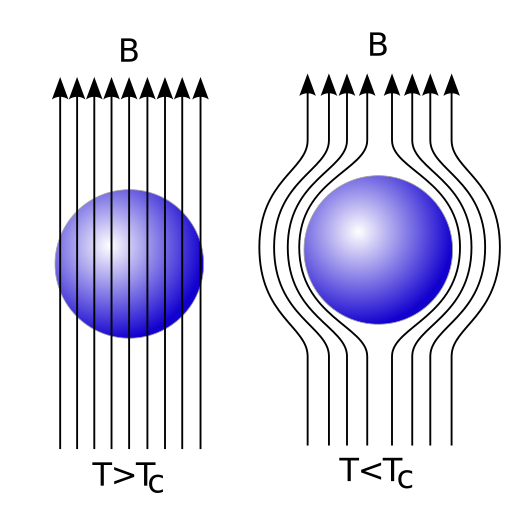
\includegraphics[width=120mm,angle=0,clip=,scale=0.5]{IMG/Meissner.png}
	}
	\caption{Rappresentazione di quello che avviene alle linee di campo magnetico per $T<T_C$}
	\label{MEIS:FIG}
\end{figure}

\subsubsection{Calore specifico}
Dal punto di vista della comprensione microscopica della superconduttivit\`a, fu particolarmente importante osservare la curva di calore specifico di un materiale superconduttore.
\begin{figure}
	\centering
	\fbox{
		\begin{tikzpicture}[scale=1,auto=center]
			\draw[->] (-2,0) -- (2,0);
			\draw[->] (-2,0) -- (-2,5);
			\node[] at (2,-0.25) {$T$};
			\node[] at (-2.5,5) {$C_v(T)$};
			\draw[domain=-2:0] plot (\x,{1.91^(\x+2)-1});
			\draw[domain=0:2] plot (\x,{0.7*\x+(2*0.7)});
			\draw[<->,dashed] (0,1.91^2-1) -- (0,-0.5); 
			\node[] at (0,-0.7) {$T_C$};
		\end{tikzpicture}
	}
	\caption{Calore specifico per un superconduttore}
	\label{SUPER:CAL:SP}
\end{figure}
Come \`e possibile osservare in Fig.~\ref{SUPER:CAL:SP}, per $T<T_C$ il calore spercifico ha un'andamento esponenziale, mentre per $T>T_C$ di tipo lineare. Questo si presta ad una interpretazione davvero affascinante in quanto \`e un diretto richiamo al modello di \textit{Cristallo di Einstein}, in pi\`u il fatto che in $T=T_C$ sia presente una discontinuit\`a, fa pensare che \textit{da qualche parte}, sia presente un gap nello spettro di energie. A chiarire questi dubbi sar\`a direttamente la teoria microscopica di BCS. La parte esponenziale per temperature inferiori alla temperatura critica, si vedr\`a essere diretta causa del fatto che la superconduttivit\`a \`e strettamente legata al verificarsi di una interazione attrattiva tra di elettroni, vicnini alla superficie di fermi, mediata da un fonone.

\subsubsection{Principio isotopico}
Il principio isotopico \`e una ulteriore prova sperimentale che il fenomeno della presenza di portatori di carica, che generano la \textit{superconrrente}, \`e strettamente legato alle interazioni col reticolo. Sperimentalmente si osserva che la temperatura critica e la massa ionica sono correlate tra loro da una legge di tipo
\newl{T_C = \frac{1}{\sqrt{M^{a^+}}}.}
Come mostrato dall'andamento del calore specifico, anche questo fatto, indica che alla base del fenomeno ci deve essere una stretta interazione col reticolo cristallino, in particolar modo, come si vedr\`a, una interazione tra gli elettroni, mediata dal fonone.

\subsubsection{Esistenza di due tipi di superconduttori}
Altra importante evidenza fenomenologica, consiste nell'esistenza di due tipi differenti di superconduttori e che il fenomeno della superconduttivit\`a \`e legato anche ad un campo mangetico critico, da cui dipende $T_C$.
Come si pu\`o notare in Fig.~\ref{SUPER:TIPI2} sono rappresentati i comportamenti dei due tipi differenti di superconduttori. Nei superconduttori di tipo II, quando si \`e tra la regione compresa tra i due campi magnetici critici, si ha uno stato misto, in cui il materiale \`e si un superconduttore ma si ha penetrazione di campo magnetico. In questa situzione di presentano i noti vortici di Abrikosov. 
\begin{figure}[H]
	\centering
	\begin{subfigure}[b]{0.4\textwidth}
	\fbox{
		\begin{tikzpicture}[scale=1,auto=center]
			\draw[->] (-2,0) -- (2,0);
			\draw[->] (-2,0) -- (-2,5);
			\node[] at (2,-0.25) {$T$};
			\node[] at (-2.75,5) {$H$};
			\draw[domain=-2:0] plot (\x,{-0.5*(\x+2)^2 +2});
			\draw[<->,dashed] (0,0.5) -- (0,-0.5); 
			\node[] at (0,-0.7) {$T_C$};
			\node[] at (-2.5,2) {$H_C$};
		\end{tikzpicture}
	}
	\caption{TIPO I - Andamento di $H_C$ in funtione a $T$. Diamagnete perfetto, completo effetto Maissner}
	\end{subfigure}
	\qquad\quad
	\begin{subfigure}[b]{0.4\textwidth}
	\fbox{
		\begin{tikzpicture}[scale=1,auto=center]
			\draw[->] (-2,0) -- (2,0);
			\draw[->] (-2,0) -- (-2,5);
			\node[] at (2,-0.25) {$T$};
			\node[] at (-2.75,5) {$H$};
			\draw[domain=-2:0] plot (\x,{-0.5*(\x+2)^2 +2});
			\draw[domain=-2:0] plot (\x,{-(\x+2)^2 +4});
			\draw[<->,dashed] (0,0.5) -- (0,-0.5); 
			\node[] at (0,-0.7) {$T_C$};
			\node[] at (-2.5,2) {$H_{C1}$};
			\node[] at (-2.5,4) {$H_{C2}$};
		\end{tikzpicture}
	}
	\caption{TIPO II - Andamento di $H_C$ in funtione a $T$. Creazione di uno stato misto. vortici di Abrikosov}
	\end{subfigure}
	\qquad\quad
        \begin{subfigure}[b]{0.4\textwidth}
	\fbox{
		\begin{tikzpicture}[scale=1,auto=center]
			\draw[->] (-2,0) -- (2,0);
			\draw[->] (-2,0) -- (-2,5);
			\node[] at (2,-0.25) {$H$};
			\node[] at (-2.75,5) {$-4\pi M$};
			\draw[domain=-2:0] plot (\x,{\x+2});
			\draw[<->,dashed] (0,1.91^2-1) -- (0,-0.5); 
			\node[] at (0,-0.7) {$H_C$};
		\end{tikzpicture}
	}
	\caption{TIPO I - Andamento della Magnetizzazione n funzione di $H$}
	\end{subfigure}
	\qquad\quad
        \begin{subfigure}[b]{0.4\textwidth}
	\fbox{
		\begin{tikzpicture}[scale=1,auto=center]
			\draw[->] (-2,0) -- (2,0);
			\draw[->] (-2,0) -- (-2,5);
			\node[] at (2,-0.25) {$H$};
			\node[] at (-2.75,5) {$-4\pi M$};
			\draw[domain=-2:0] plot (\x,{\x+2});
			\draw[domain=0:1] plot (\x,{2/(\x+1)});
			\draw[<->,dashed] (0,1.91^2-1) -- (0,-0.5); 
			\draw[<->,dashed] (1,1.91^2-1) -- (1,-0.5);
			\node[] at (0,-0.7) {$H_{C1}$};
			\node[] at (1,-0.7) {$H_{C2}$};
		\end{tikzpicture}
	}
	\caption{TIPO II - Andamento della Magnetizzazione n funzione di $H$}
	\end{subfigure}
	\caption{Comportamenti differenti dei due tipi di superconduttori}
	\label{SUPER:TIPI2}
\end{figure}

\subsubsection{Esistenza delle correnti persistenti - Intrappolamento di flusso di campo magnetico}
Una ulteriore prova dell'esistenza del fenomeno della superconduttivit\`a sono le \textit{correnti persistenti}. Supponiamo di prendere un anello di materiale superconduttore in equilibrio, immergiamolo in un campo magnetico, per effetto Meissner, si verr\`a a creare una corrente in modo tare che si venga a creare un campo magnetico che annulli quello interno. In questo regime, supponiamo di spegnere il campo magnetico esterno, quello che si verifica \`e che la corrente, non trovando modo di dissiparsi, continua a viaggiare nel materiale superconduttivo intrappolando tra la sua area, una cerca quantit\`a di campo magnetico. Si misura sperimentalmente che la quantit\`a di flusso concatenato, dovuto alle correnti persistenti \`e \textbf{quantizzato} e proporzionale a
\newl{\Phi=\frac{hc}{2e}.}
Questo risultato \`e particolarmente importante e sar\`a necessario per effettuare dei ragionamenti sulle teorie fenomenologiche che verranno esposte nel prossimo paragrafo.
\subsection{Teoria Fenomenologica di London}
La teoria fenomenologica di London \`e la prima proposta di spiegazione di spiegazione del fenomeno della superconduttivit\`a. Come sar\`a possibile vedere, presenta numerosi limiti e non spiega tutte le evidenze fenomenologiche ma deriva in modo molto preciso l'effetto Maissner per i superconduttori di tipo-I e il fatto che il flusso di campo magnetico intrappolato \`e quantizzato. Di notevole importanza sar\`a osservare la usa forma, molto simile a quella sperimentale, ma differente in un dettaglio sostanziale. London, inizia considerando che nel materiale superconduttore in studio, ci sia una certa porzione di elettroni che rappresentano i portatori di carica della supercorrente. Per semplicit\`a si identifichi questa densit\`a di super-elettroni con $n_s$, quindi la densit\`a di supercorrente \`e $J=-n_s e v$.  Si consideri che la super-corrente identificata da questi elettroni sia un fluido incomprimibile, quindi $\nabla J = 0$. Per descrivera la dinamica dei super-elettroni, si usi la legge di Lorentz
\newl{\frac{dv}{dt} = -\frac{e}{m}\left[E+\frac{1}{c}v\times B \right], }
che sviluppando la derivata totale di $v$ diventa:
\newl{\frac{dv}{dt}  + \nabla\left(\frac{1}{2}v^2\right) - v\times(\nabla \times v) = -\frac{e}{m}\left[E+\frac{1}{c}v\times B \right]. }
Riordinando semplicemente i termini
\newl{\frac{dv}{dt} + \nabla\left(\frac{1}{2} v^2\right) = -\frac{e}{m} E + v\times\left[ \nabla \times v -\frac{e}{mc}B  \right]   
	\label{LOR:SUP}
}
Si definisce Bulk della Superconduttivit\`a  la quantit\`a $Q= \nabla \times v -e/(mc)B$. Usando la seconda eq di Maxwell $\nabla \times E = -(1/c) (\partial_t B)$ \`e possibile scrivere
\newl{\frac{\partial Q}{\partial t} = \nabla \times (v\times Q).
	\label{EQUIL:SUP}
}
\`E possibile ora fare alcuni ragionamenti sulla quantit\`a $Q$. In assenza di campo magnetico, col materiale superconduttore in equilibrio, \`e sostanzialmente tutto fermo e la quantit\`a $Q=0$. Applicando un campo magnetico si ha che per effetto Maissner il superconduttore raggiunge un suo equilibrio, l'Eq.~(\ref{EQUIL:SUP}) ci indica che l'equilibrio raggiunto \`e totalmente trasparente al modo in cui lo si \`e raggiunto, quindi $Q$ rimane sempre nulla per ogni superconduttore all'equilibrio. In questo modo abbiamo le \textit{equazioni di London}, la prima deriva dal fatto che per ogni superconduttore si ha che $Q=0$,
\newl{\textbf{I Eq. London }\boxed{\nabla \times v - \frac{e}{mc}B=0.} \label{PRIM:EQ:L} }
La seconda equazione di London si determina semplicemente inserendo l'Eq.~(\ref{PRIM:EQ:L}) nel'Eq.~(\ref{LOR:SUP}) ottenendo
\newl{\textbf{II Eq. London }\boxed{\frac{dv}{dt} + \nabla\left(\frac{1}{2} v^2\right) = -\frac{e}{m}E}}
\subsubsection{Risultati della Teoria di London}
Dalla prima equazione di London si deriva subito un risultato molto importante sull'effetto Maissner. Prendiamo l'Eq.(\ref{PRIM:EQ:L}), scrivendola in funzione di $J$ compaiono una densit\`a di super-elettroni e una carica elettrica. Il rotore di $J$ \`e un laplaciano con un fattore $4\pi$. Detto questo, la prima equazione di London pu\`o essere riscritta come
\newl{\nabla^2 B(x) = \frac{mc}{4\pi n_s e^2 }B(x),}
La cui soluzione \`e particolarmente semplice
\newl{B(x) =B_0 e^{-\frac{x}{\lambda_L} },}
dove $\lambda_L$ \`e la lunghezza di penetrazione di London che nell'ordine di $\lambda_L\sim50nm$.

Sempre la prima equazione di London fornisce un'informazione molto importante sul momento dei super-elettroni. Sostituendo semplicemente, $\nabla \times A = B$ nella prima equazione di London, si ottiene che:
\newl{\nabla \times \left(p-\frac{e}{c}A\right)= \nabla \times P = 0, \label{ROT:MOM:NUL}}
che \`e un risultato che servir\`a tra poco.
Si consideri ora la seconda equazione di London linearizzata, quindi consideriamo di eliminare il termine in $\nabla v^2$
\newl{\frac{dv}{dt} = -\frac{e}{m} E, }
usando la seconda equazione di Maxwell e considerando la derivata rispetto alla densit\`a di corrente, anzich\`e le sole velocit\`a la scrittura si arricchisce divendando
\newl{\nabla\times\frac{dJ}{dt} = \frac{n_se^2}{mc}\frac{\partial B}{\partial t}.}
Integrando sulla superficie attraversata dal campo magnetico si ottiene
\newl{\int_{\Sigma} \left(\nabla\times\frac{dJ}{dt}\right) d\Sigma - \frac{n_se^2}{mc}\int_{\Sigma} \left(\frac{\partial B}{\partial t}\right) d\Sigma =0   
\\
\oint_{\gamma} \frac{dJ}{dt} dl - \frac{n_se^2}{mc} \int_{\Sigma} \left(\frac{\partial B}{\partial t}\right) d\Sigma =0
\\
\frac{d}{dt}\left( \int_{\Sigma} B \cdot d\Sigma -\frac{mc}{n_se^2}\oint_{\gamma} J \cdot dl \right)=0.
}
Si definisce \textit{FLUSSOIDE}, e lo si indica con la lettera $\Phi$, la quantit\`a
\newl{\Phi=\int_{\Sigma} B \cdot d\Sigma -\frac{mc}{n_se^2}\oint_{\gamma} J \cdot dl. \label{FLUSSOIDE}}
Ricordando l'Eq.~(\ref{ROT:MOM:NUL}) e usandola nell'Eq.~(\ref{FLUSSOIDE}) otteniamo uno dei risultati pi\`u importanti della teoria di London, cio\`e che il flusso di campo mangetico, in un superconduttore, \`e quantizzato. Facendo il conto si ottiene
\newl{\Phi_L=\int_{\Sigma} B \cdot d\Sigma -\frac{mc}{n_se^2}\oint_{\gamma} J \cdot dl = \int_\Sigma \left(\nabla\times A\right)\cdot d\Sigma - \frac{mc}{e}\oint_{\gamma} v\cdot dl = 
\\
=\oint_{\gamma} A \cdot dl - \frac{mc}{e}\oint_{\gamma} v\cdot dl = \oint_{\gamma}\left(A - \frac{mc}{e} v\right)\cdot dl =
\\
=-\frac{c}{e}\oint_{\gamma} \left(mv - \frac{e}{c} A\right) dl = -\frac{c}{e}\int_\Sigma\left( \nabla \times P\right) d\Sigma.
}
Dato che $\nabla\times P = 0$, l'ultimo passaggio ci indica che $\Phi$ \`e una costante. Applicando il teorema di Stokes, si ottiene esattamente l'equazione di Bohr-Sommerfeld per l'azione ridotta quantistica
\newl{\Phi_L=-\frac{e}{c}\int_\Sigma\left( \nabla \times P\right) d\Sigma= -\frac{c}{e} \oint_{\gamma}P\cdot dl = \frac{c}{e}2\pi \hbar n}
L'equazione di Bohr-Sommerfeld ha come autovalori multipli di $\hbar$, quindi risulter\`a che il flusso sar\`a multiplo di
\newl{\boxed{\Phi_L = \frac{hc}{e}.}}
\subsubsection{Conclusioni sulla teoria di London}
Come \`e stato possibile vedere, la teoria di London prevede bene l'esistenza dei superconduttori di tipo-I soggetti ad effetto Maissner. Prevede che la quantizzazione del flusso di campo magnetico intrappolato nel superconduttore, ma \`e sbagliato di un fattore due. Infatti, ricordando i risultati fenomenologici ottenuti con la misura del campo magnetico intrappolato in una anello superconduttore si ha che 
\newl{\boxed{\Phi_{sperimentale} = 2\Phi_L.}}
In questa relazione \`e riassunto il grande limite della teoria. Non spiega chi sono i portatori di carica. Non sono elettroni, sono un qualcosa con carica doppia dell'elettrone. Nonostante siano gi\`a in questo modo evidenti alcuni aspetti della superconduttivit\`a, il fatto che non siano previsti superconduttori di tipo-II e il fatto che non si riesca a valutare la natura dei portatori di carica, suggerisce il fatto che l'approcio classico al problema \`e sbagliato. Nel prossimo paragrafo si vedr\`a come questa teoria fenomenologica, pu\`o essere corretta, e raffinata inserendo le correzioni di Ginzburg-Landau all'energia libera. Nonostante gli sforzi, rimane concettualmente sbagliato il punto di partenza semi-classico di queste teoria.
\subsection{Le equazioni di Pippard}
Come visto nel precedente paragrafo, la teoria fenomenologica di London ha dei limiti abbastanza grossolani. Il risultato sul flussoide, scalato di un fattore due, dal punto di vista di una teoria fenomenologica, era un problema facilmente risolvibile attraverso l'introduzione di grandezze efficaci. Il limite pi\`u grande della teoria riguarda appunto la mancata previsione dei superconduttori di tipo-II. Si introdue il cos\`i detto gauge di London
\newl{
\nabla \cdot A = 0\nonumber\\
A\cdot n = 0.
\label{GAUGE:LOND}
}
In questo gauge, la prima equazione di London diventa
\newl{
	\int_{\Sigma}\left( \nabla \times J\right)\, d\Sigma = -\frac{n_s e^2}{mc}\int_{\Sigma}\left(\nabla \times A\right)\, d\Sigma \nonumber\\
	\int_{\gamma} J \cdot dl = -\frac{n_s e^2}{mc} \int_{\gamma} A \cdot dl\nonumber\\
	J(x) = - \frac{n_s e^2}{mc} A(x).
	\label{SUPERCORRENTE}
}
Si ha quindi una realzione tra la densit\`a di corrente e il potenziale vettore nello stesso punto. Gli studi di Pippard lo portarono a concludere che la lunghezza di penetrazione del campo mangetico nel superconduttore non \`e una costante. Secondo la teoria di London, cambiare la penetrazione di campo magnetico voleva dire cambiare il numero di$ n_s$, quindi stravolgere in modo sensibile le propriet\`a termodinache dei superconduttori. Pippard propone una lettura della supercorrente in Eq.~\ref{SUPERCORRENTE} in modo locale, dove la $J(x)$ \`e in funzione ad un campo medio di $A(x)$ primo vicino di dimensione $r_0$. Per elementi adeguatamente dopati, $r_0$ \`e paragonabile al cammino medio di un elettrone libero $l$, nel caso dei metalli Pippard definisce una \textit{lunghezza di correlazione} identificata con $\xi_0$. La relazione di Pippard lega insieme $r_0$, $l$ e $\xi_0$
\newl{\frac{1}{r_0}=\frac{1}{l}+\frac{1}{\xi_0} }
la densit\`a di supercorrente \`e possibile considerarla come
\newl{J(x) = -\frac{n_S e^2}{mc} \frac{3}{4\pi \xi_0} \int d^3x\, \frac{X[X\cdot A(x')]t}{\abs{X} ^4} e^{-x/r_0} }





\subsection{Teoria fenomenologica di Ginzburg-Landau}
Come \`e stato possibile osservare nel paragrafo precedente, la teoria fenomenologica di London ha alcuni limiti come la mancata previsione dell'esistenza dei superconduttori di tipo-II e l'errata stima del flussoide di un fattore 2. Lo stesso London aveva notato questo limite ad esempio nelle giunzioni (sia tra due superconduttori che tra un superconduttore e un materiale normale). Quando lo strato di separazione tra i due layer della giunzione diventava molto piccolo sostanzialmente era impossibile da spiegare il fatto che la superficie di energia diventava positiva. London cerc\`o di valutarne l'entit\`a tramite degli studi fatti su giunzioni Sn-In, anche se una iniziale trattazione, sempre fenomenologica, fu fatta da Ginzburg-Landau.
\subsubsection{Espanzione dell'energia libera}
L'energia libera di un superconduttore $F_s(T,H)$ dipender\`a dalla temperatura e dal campo magnetico applicato. Il superconduttore \`e un perfetto diamagnete, quindi il contributo dato da $H$ sar\`a puramente diamagnetico, permettendo quindi di scrivere
\newl{F_S(T,H) \sim F_S(T,0)+\frac{H^2}{8\pi}.}
Si consideri ora l'energia libera di un materiale normale e la si identifichi con $F_N(T,H)$. Anche lei dipender\`a dalla temperatura e dal campo magnetico. Per $T > T_C$ il contributo magnetico \`e molto piccolo, quindi trascurabile permettendo di scrivere
\newl{F_N(T,H)\sim F_N(T,0).}
Per $T\sim T_C$ si ha che $F_N \sim F_S$ quindi
\newl{
	F_S(T,H) \sim F_N(T,0) + \frac{H^2}{8\pi}. 
	\label{EN:LIB}	
}
La proposta di Ginzburg-Landau \`e quella di descrivere l'energia libera di un superconduttore in funzione ad un parametro complesso d'ordine che definiamo essere $\Psi(x)$. Il modulo di $\abs{\Psi} $ ha la propriet\`a di essere piccolo per $T\sim T_C$ quindi l'energia libera in Eq.~\ref{EN:LIB}, in assenza di campo magnetico, \`e possibile descriverla come sviluppo in funzione del parametro d'ordine
\newl{
	F_S(T,0) = F_N(T,0) + a \abs{\Psi} ^2 + \frac{b}{2} \abs{\Psi} ^4 +\cdots,
	\label{SVILUPPO:GL}
}
in cui $a$ e $b$ sono due costanti fenomenologiche dipendenti dalla temperatura. Ginzburg e Landau, analogamente all'equazione di Schoedinger, aggiungono allo sviluppo un termine di ordine $\abs{\nabla \psi} ^2$ che ha appunto la forma
\newl{(2m^*)^{-1}\abs{\left(-i\hbar\nabla+\frac{e^*}{c}A\right) \Psi } ^2.  }
Riutilizzando tutti i risultati nell'Eq.~\ref{SVILUPPO:GL}, si ottiene
\newl{F_S = F_{N,0} + a \abs{\Psi} ^2 + \frac{b}{2} \abs{\Psi} ^4 + (2m^*)^{-1}\abs{\left(-i\hbar\nabla+\frac{e^*}{c}A\right) \Psi } ^2 + \frac{H^2}{8\pi}}
in cui, tutte le grandezze asteriscate sono delle grandezze efficaci definite come
\newl{
	m^* = 2m_e \nonumber\\
	e^* = 2e   \nonumber\\
	\abs{\Psi} = n_s^* = \frac{1}{2}n_s \nonumber
}
dove $n_s$ rappresenta la densit\`a di elettroni coinvolti nel fenomeno della superconduzione.

























\subsection{Teoria BCS }


















\end{document}
